% !Tex root = dis.tex
\graphicspath{{./images/appendix3/}}
\chapter{Measuring the Cognitive Load of Code: }

Investigating the use of CLT techniques to minimize debugging time and errors

\section{Review}

As I established at the beginning of this dissertation, Cognitive Load Theory is a fruitful field of principles from instructional and user interface design that lies fallow for software engineering. Professional software engineering involves many non-programming related activities, but the core unifying glue is always code. As software engineering practitioner literature has argued, code that is poorly written and difficult to understand can cost companies time, money, and even--such as in the case of the HEARTBLEED OpenSSL bug-- expose massive security vulnerabilities just due to a missing set of “{ }” for an if-statement.

Code style is arguably important, but attempts to analytically quantify the impact of different techniques remains more art than science. Additionally, researchers such as Lionel Briad and Ivar Jacobson have decried the lack of strong theoretical principles for software engineering. This work explores the intersection of Cognitive Load Theory and software engineering best practices to answer the question: “Is there a relationship between evidence driven best practices for organizing educational content and published best practices for writing code?”
Experiment: Fix a bug in date-time manipulation in Joda Time
I chose to apply software engineering best practice techniques identified in Clean Code and Refactoring to a popular open-source Java library called Joda-time. Joda-time is one of the most highly-used libraries in the Java ecosystem. Jodatime sits in the dependency tree of many popular software packages such as Spring, the Lift web application framework, Hibernate annotations, and many, many more. As such, this is not a contrived exercise dreamed up by a graduate student in a lab to show an effect. This is real, battle-tested, used by millions code.
 
I also chose Joda-time because it is written in Java. Java and C++ are the most well-known programming languages in the community. Java is taught in many college curriculums; finding familiar programmers is less difficult than other languages. Joda-time solves a very general problem--date \& time manipulation. Most languages have date libraries for common operations like arithmetic, formatting, or timezone conversion. Good and usable libraries provide broad, usable abstractions for complicated functionality. Date \& Time manipulation is very complicated, often causing bugs even in major professional software engineering environments. 

\section{Bug: ISO8601 Years}

The “devil in the detail” is all of the edge cases. One of the devilish details is the existence of a large, amorphous, ever-changing set of formats describing a date. The International Standards Organization attempted to ameliorate this with ISO8601, which defines a canonical format for the interchange of dates and times across locales. One of the quirks of the standard is that the published format is YYYY-MM-DD, however, the standard allows for more than 4-digit years in cases where sender and receiver have agreed upon extra digits by prepending with a + or - [$\pm$ YYYYY].

Jodatime did not originally account for this. This led to https://github.com/JodaOrg/joda-time/issues/86. Hari Shankar explored the depths of the code and identified an issue and a fix. He did not report how long it took to find the bug, or how difficult it was to come up with a solution. When I first found this issue, it was still open. In October of 2015, Steven Colebourne (primary author/maintainer of the library) merged in Shankar’s fix.

\section{Analysis of Accepted Solution}

The accepted solution follows a common maintenance programmer practice: change as little code as possible and duplicate where necessary and with slight tweaks to achieve desired behavior. It is not exactly but similar in vein to “Programming By Difference.” It is a conservative approach that tends to be favored when code is in obsolescence, has a large number of consumers, or is otherwise hard to change.  

“Other reasons” that code can be hard to change include a lack of confidence in correct behavior, or difficulty in understanding algorithms and data structures written by someone else. The commit that introduced the fix included unit test cases that manifest the bug (though notably only try 5 digit years, perhaps not fully exercising failure modes), suggesting the maintainer understood the code enough to augment the existing test suite, a software best practice. The original code was not written solely by Stephen Colebourne. Attribution information in the comments suggests it was a collaborative effort between Colebourne, Brian S. O’Neill, and Fredrik Borgh. It’s possible this had an effect on the aggressiveness of the fix.

Using SonarQube 5.4 for analysis, we find that the DateTimeFormatterBuilder alone has 1600 LoC. 2625 total lines (including comments) with 162 issues found via static source analysis, with 2.3\% duplications, estimated to take 2.5 days to fix. It has a Cyclomatic Complexity score of 550, the highest in the library.

When gathering statistics of the library with the “Run Tests with Coverage” option of IDEA IntelliJ, Joda Time exhibits an impressing 98\% class/91\% line/90\% method coverage. Such a high level of coverage potentially provides developers the option to experiment with more drastic structural Refactoring and verify existing behavior, but time and other issues may not always make such re-architecture possible.



\section{Experiment: contrast debugging time and performance of accepted solution versus CLT optimized}

For the purposes of this experiment, we hold the state of JodaTime as reflected in Git commit on August 2nd 2015 as the “control” group, not including the given fix. We use the provided fix as the “gold standard”, as it was accepted by the core library contributor. We follow a 2x2 factorial design where we account for novice/expert and control/experimental for debugging time, number of defects introduced as measured by failing tests, and perceived cognitive load as measured on our Likert Scale. 

With such setup in mind, I will proceed to show how I applied software engineering best practices influenced by Cognitive Load Theory to develop the experimental treatment.

\section{Development of Experimental Version}

\subsection{Starting small: sequencing, chunking, and intrinsic complexity at the variable and method level}
I began with trying to simplify a complicated if-statement that included assignment, array indexing, and bounding checking in one compound predicate. I was guided by the presence of a comment. Robert Martin’s Clean Code suggests that “Comments are Lies.” They often become out of date as code changes with time. 

Comments also signal a failure to communicate, a missed opportunity for the code to be self-descriptive. A programmer who reads a comment incurs the additional cognitive load of reading the comment, having to verify whether it accurately summarizes the situation, and maintaining a mental mapping between the descriptive comment and the cryptic code. Cognitive Load Theory shows that redundant information adds extraneous cognitive load--learning outcomes for material that has a picture and paragraph repetitively describing the same phenomena are generally improved if the information is concisely expressed in one form. Thus, we use the technique of INTRODUCE EXPLAINING VARIABLE to make the conditional more descriptive. Realizing that these temporary variables had added lines to answer a limited scope question within the body of a method that was already 64 lines long, increasing Germane Cognitive Load for understanding the full execution of this method, I used the CLT technique of managing Germane Cognitive Load by sequencing and chunking, applying REPLACE TEMP WITH QUERY to push knowledge of this question into a cohesive chunk, a method.

\begin{figure}[H]
	\centering
	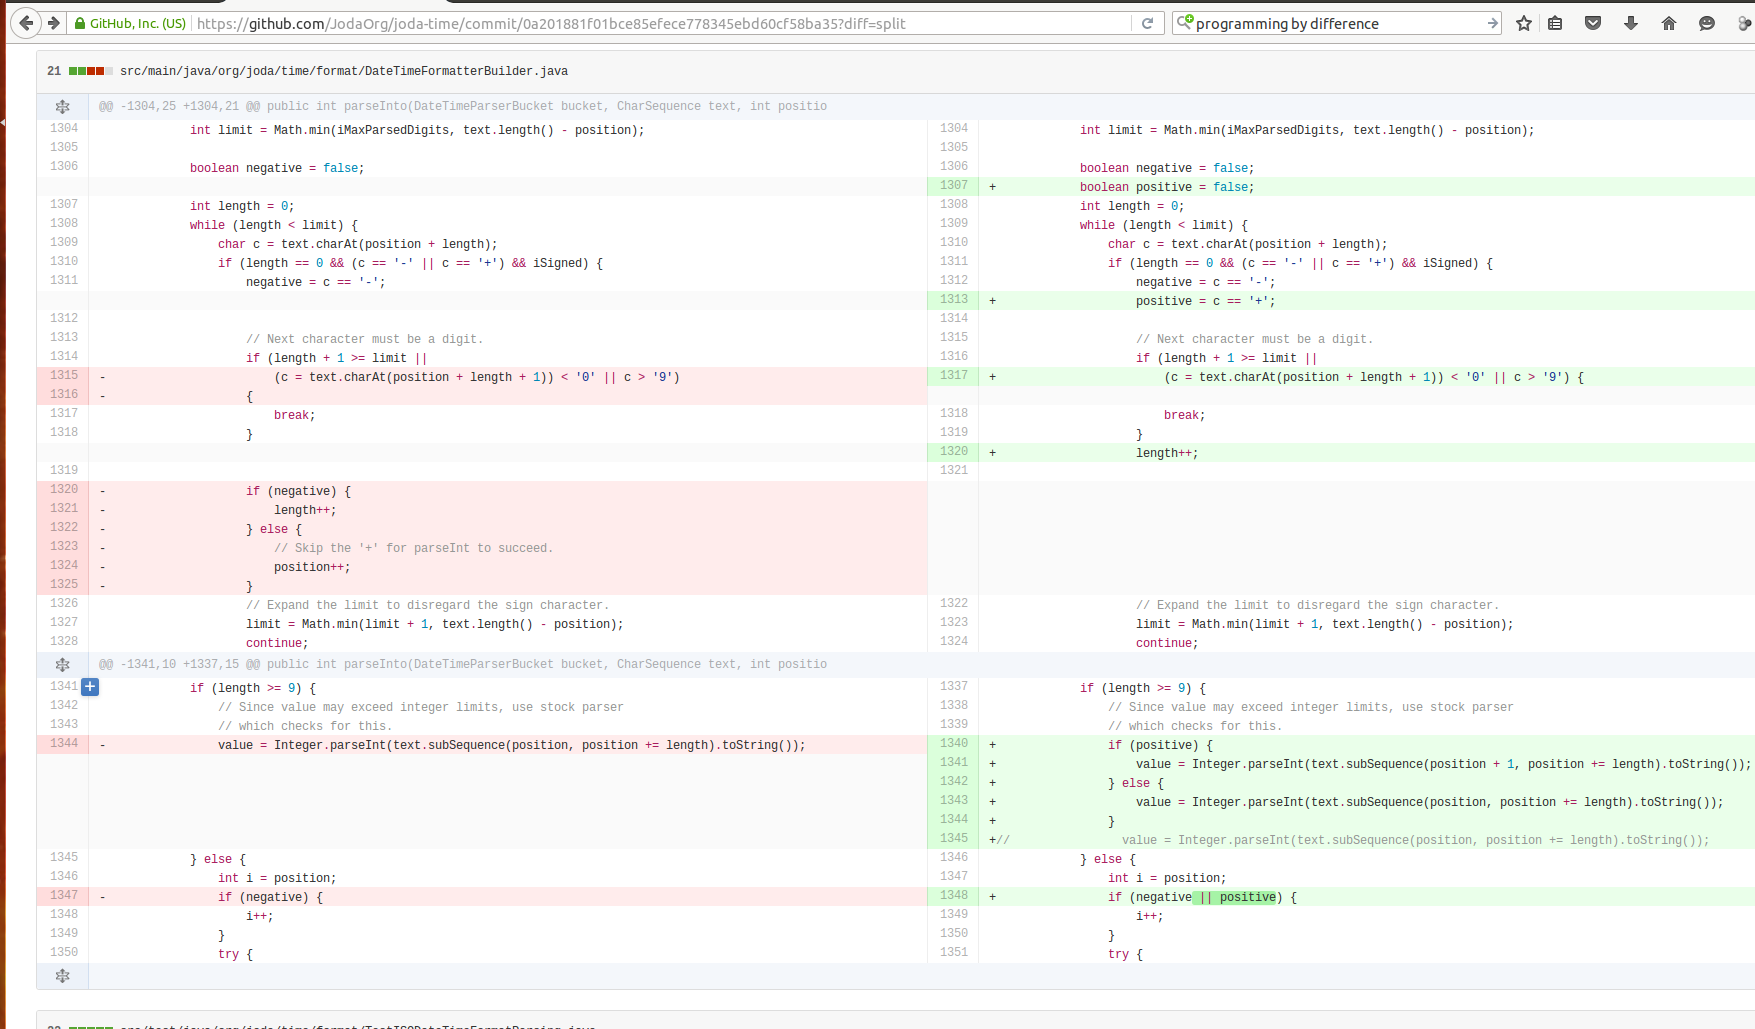
\includegraphics[width=\linewidth]{code1}
	\caption{insert caption}
\end{figure}

When I ran the tests, I discovered something troubling: a test was broken. The behavior had changed.

\texttt{Tests run: 4161, Failures: 3, Errors: 1, Skipped: 0, Time elapsed: 6.298 sec \textless \textless \textless FAILURE! - in org.joda.time.TestAllPackages}

\texttt{testFormat\_year(org.joda.time.format.TestDateTimeFormat)  Time elapsed: 0.015 sec  \textless \textless \textless ERROR!}

\texttt{java.lang.StringIndexOutOfBoundsException: String index out of range: 1}

\hspace{\parindent} \texttt{at java.lang.String.charAt(String.java:646)}

\hspace{\parindent} \texttt{at org.joda.time.format.DateTimeFormatterBuilder\$NumberFormatter.parseInto(DateTimeFormatterBuilder.java:1314)}

\hspace{\parindent} \texttt{at org.joda.time.format.DateTimeFormatter.parseDateTime(DateTimeFormatter.java:879)}

\hspace{\parindent} \texttt{at org.joda.time.format.TestDateTimeFormat.testFormat\_year(TestDateTimeFormat.java:225)}

I stared at the code for a good 20 minutes, not understanding what went wrong. Opdyke defines Refactoring as “structural code changes that exhibit no external behavioral difference.” Clearly what I’d done had ended up not being Refactoring, despite the fact that I’d leveraged the baked in functionality of IDEA IntelliJ Ultimate Edition 14, which includes a robust static analysis checker that usually detects such changes. Pouring over the expression hardly helped, the change “looked safe.” Attaching a debugger and stepping through the broken test revealed the problem.

The predicate of the if statement had caught my eye for having a lot of complexity and a comment to describe it. A hidden complexity that wasn’t immediately obvious to me was that it relied on the short-circuit evaluation behavior of the || operator in Java as an implicit GUARD CLAUSE

\texttt{length + 1 \textgreater= limit || (c = text.charAt(position + length + 1)) \textless '0' || c \textgreater '9')}

In the previous expression, the \texttt{length + 1 \textgreater= limit} prevents the \texttt{text.charAt(position + length + 1)} from being evaluated when \texttt{length + 1} would result trying to index a character outside of the string, causing an error. Thus, there is an additional semantic that provides safety based on the ordering of expressions.

This is exactly the type of hidden complexity that creates anxiety in maintenance engineers in modifying existing code. It is typified by reliance on a subtle semantic provided by the language runtime. This can be considered germane cognitive load--language semantics are part of a programmer’s toolkit. Expert programmers often use these kinds of techniques, as experts are shown to better handle an increase in germane cognitive load. Novices, however, may experience information overload.

I can simplify this by rewriting the code to be a little longer, but more explicit. 

\begin{figure}[H]
	\centering
	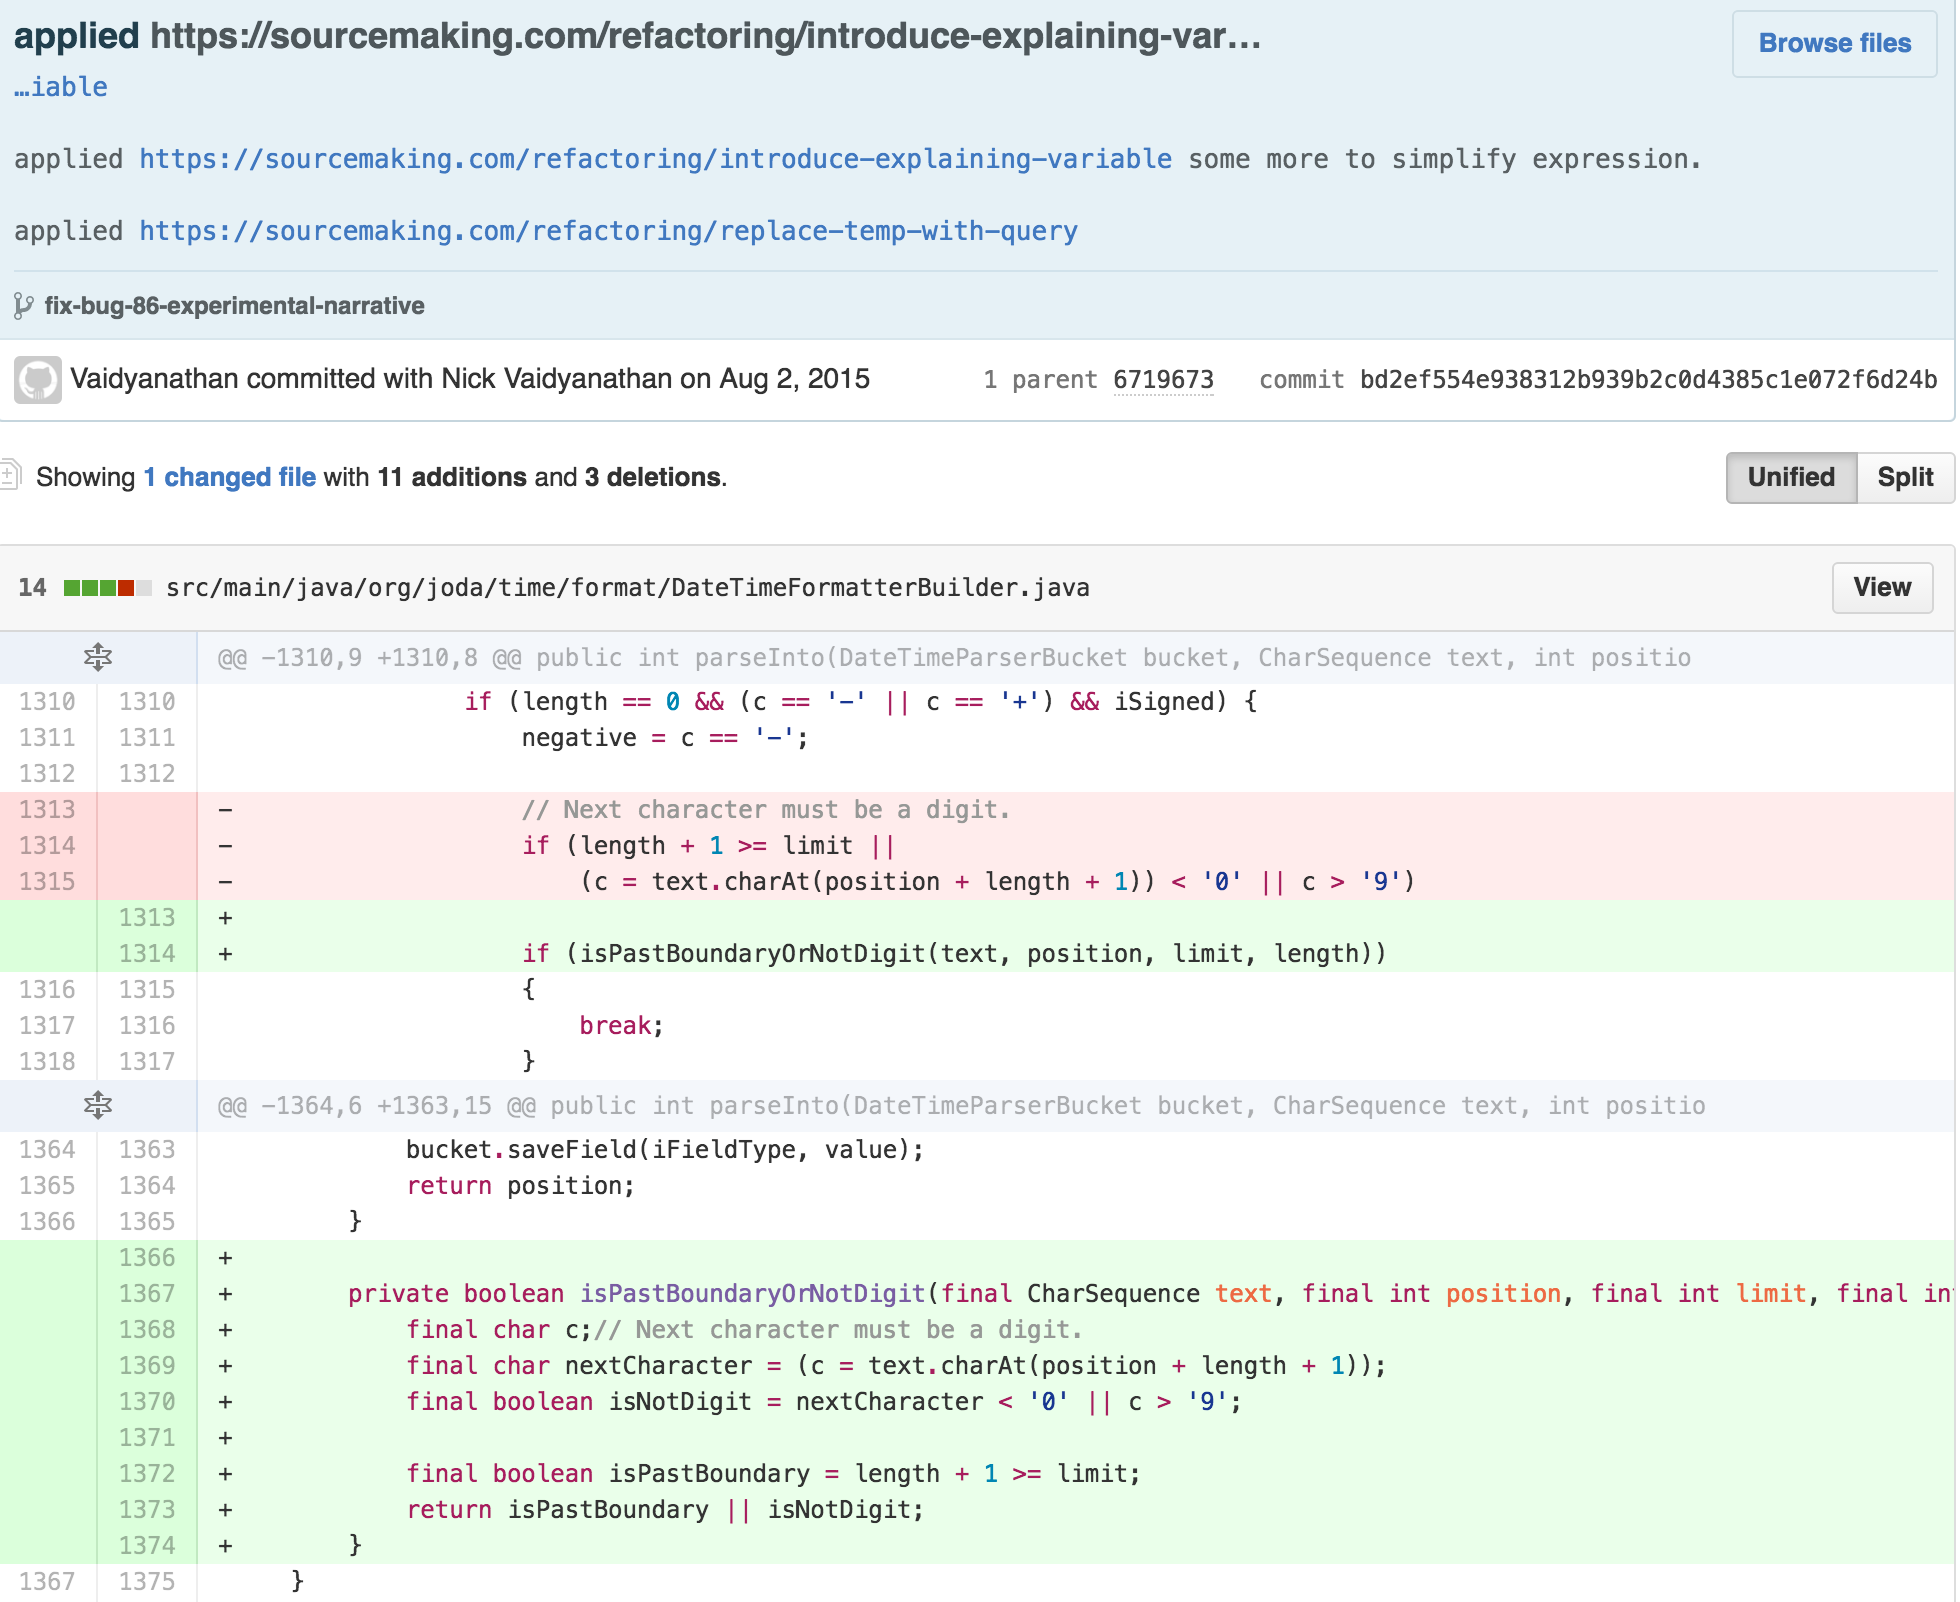
\includegraphics[width=\linewidth]{code2}
	\caption{insert caption}
\end{figure}

In this example, I make the GUARD CLAUSE more explicit and match the standard form, and use an explanatory named variables to describe the why of the calculation’s what.

\subsection{Building up: moving on to the class level}

Returning my attention to the original expression, I apply the same INTRODUCE EXPLANATORY VARIABLE and EXTRACT METHOD technique.:

\begin{figure}[H]
	\centering
	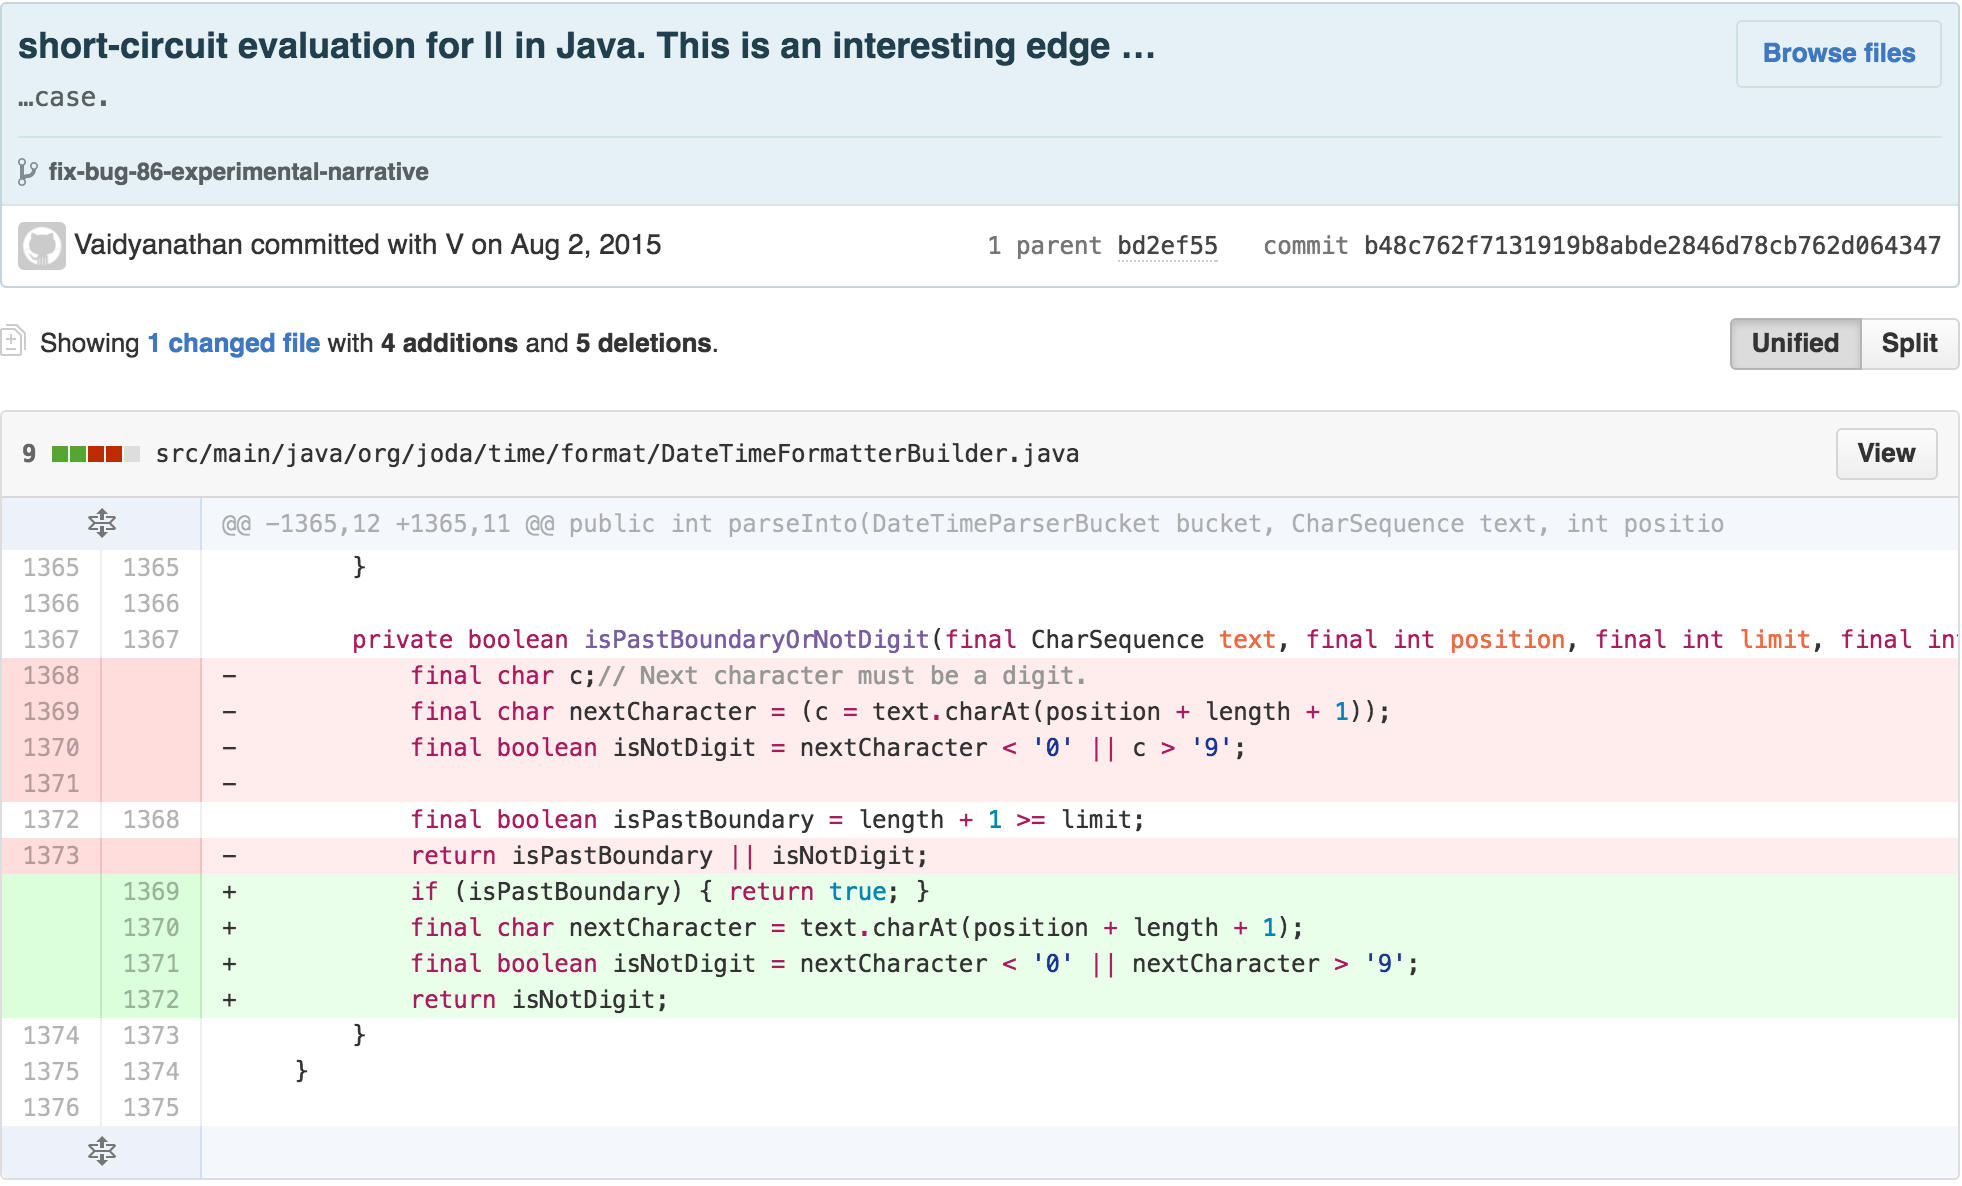
\includegraphics[width=\linewidth]{code3}
	\caption{insert caption}
\end{figure}

I also made the chunked methods static to signify that they were “pure functions.” They had no reliance on the \texttt{DateTimeFormatterBuilder}’s internal state and solely exist as calculations. This structural change helped me realize that much of the body of the \texttt{parse} method was isolated from the rest of the class. This is often an opportune situation to apply REPLACE METHOD WITH METHOD OBJECT, which can decrease the length and intrinsic cognitive load of the original class via chunking its content with the created collaborating class.

\begin{figure}[H]
	\centering
	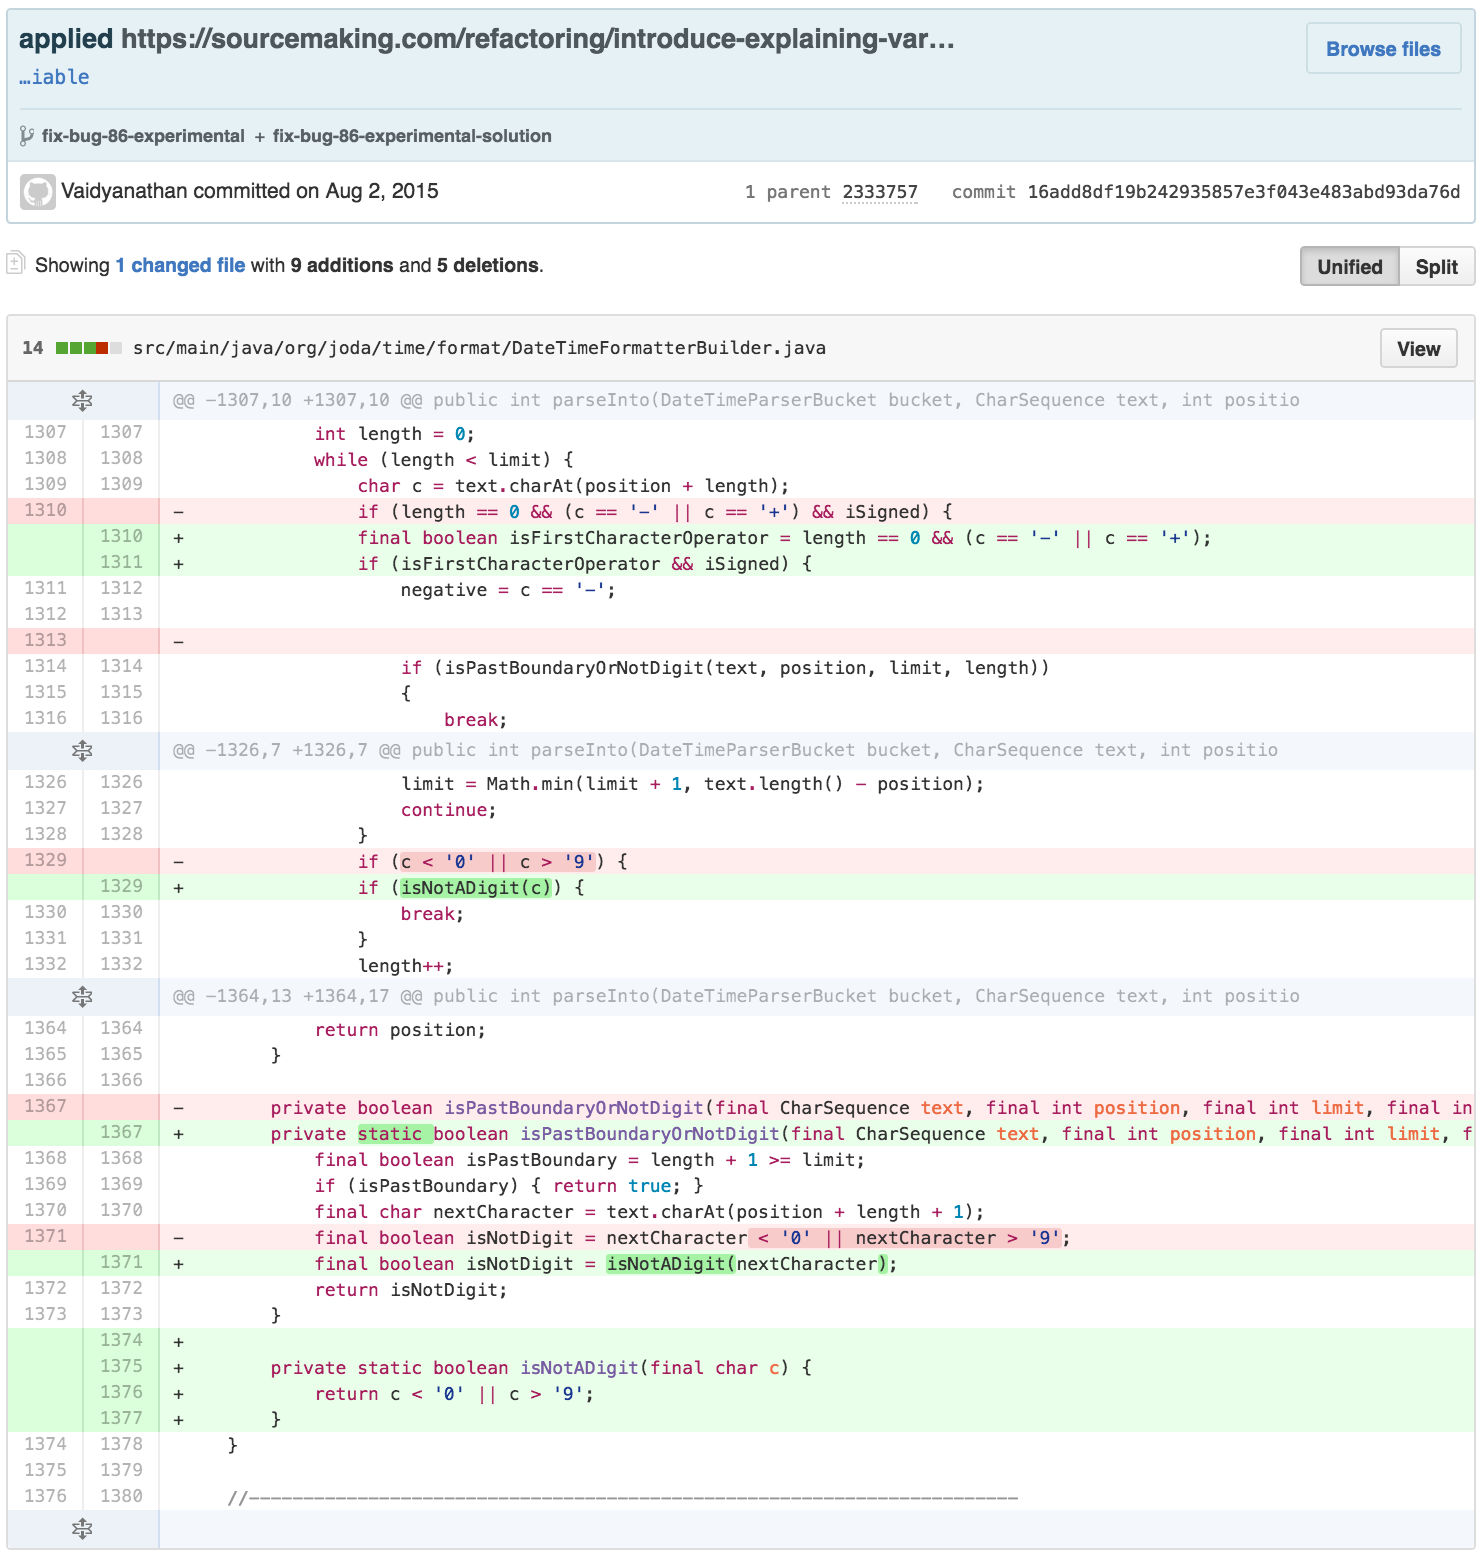
\includegraphics[width=\linewidth]{code4}
	\caption{insert caption}
\end{figure}
\begin{figure}[H]
	\centering
	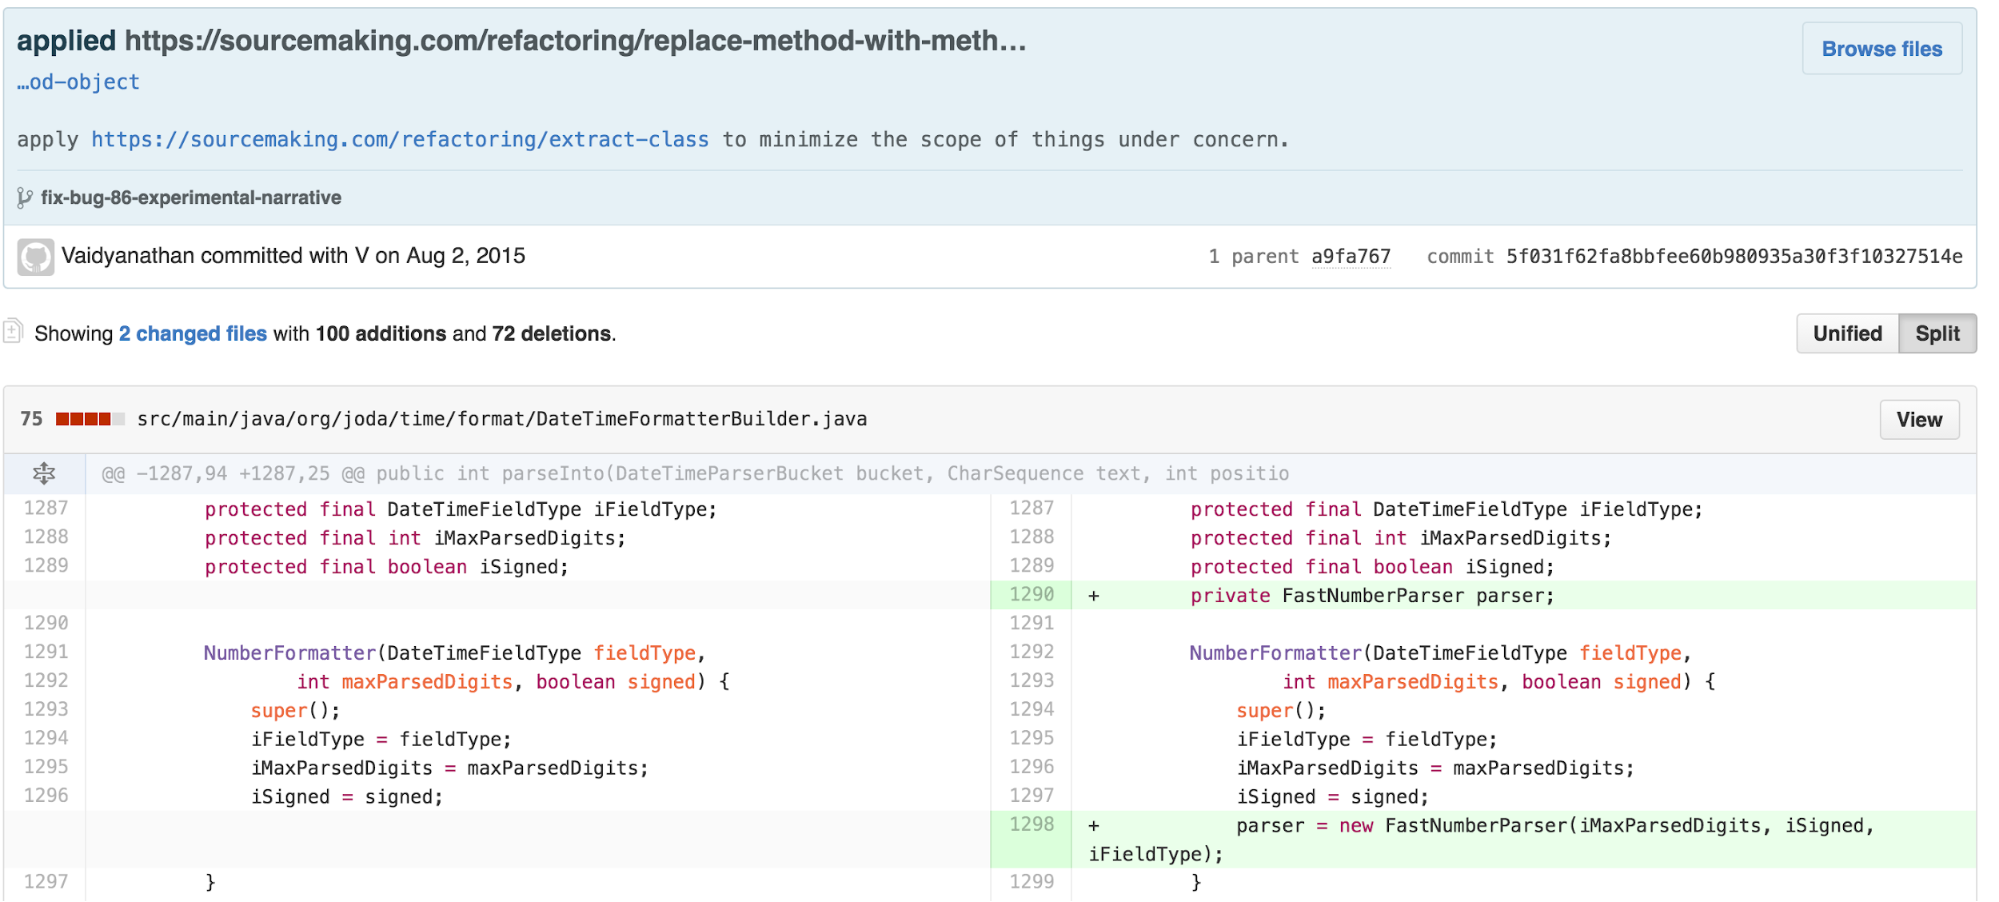
\includegraphics[width=\linewidth]{code5}
	\caption{insert caption}
\end{figure}
\begin{figure}[H]
	\centering
	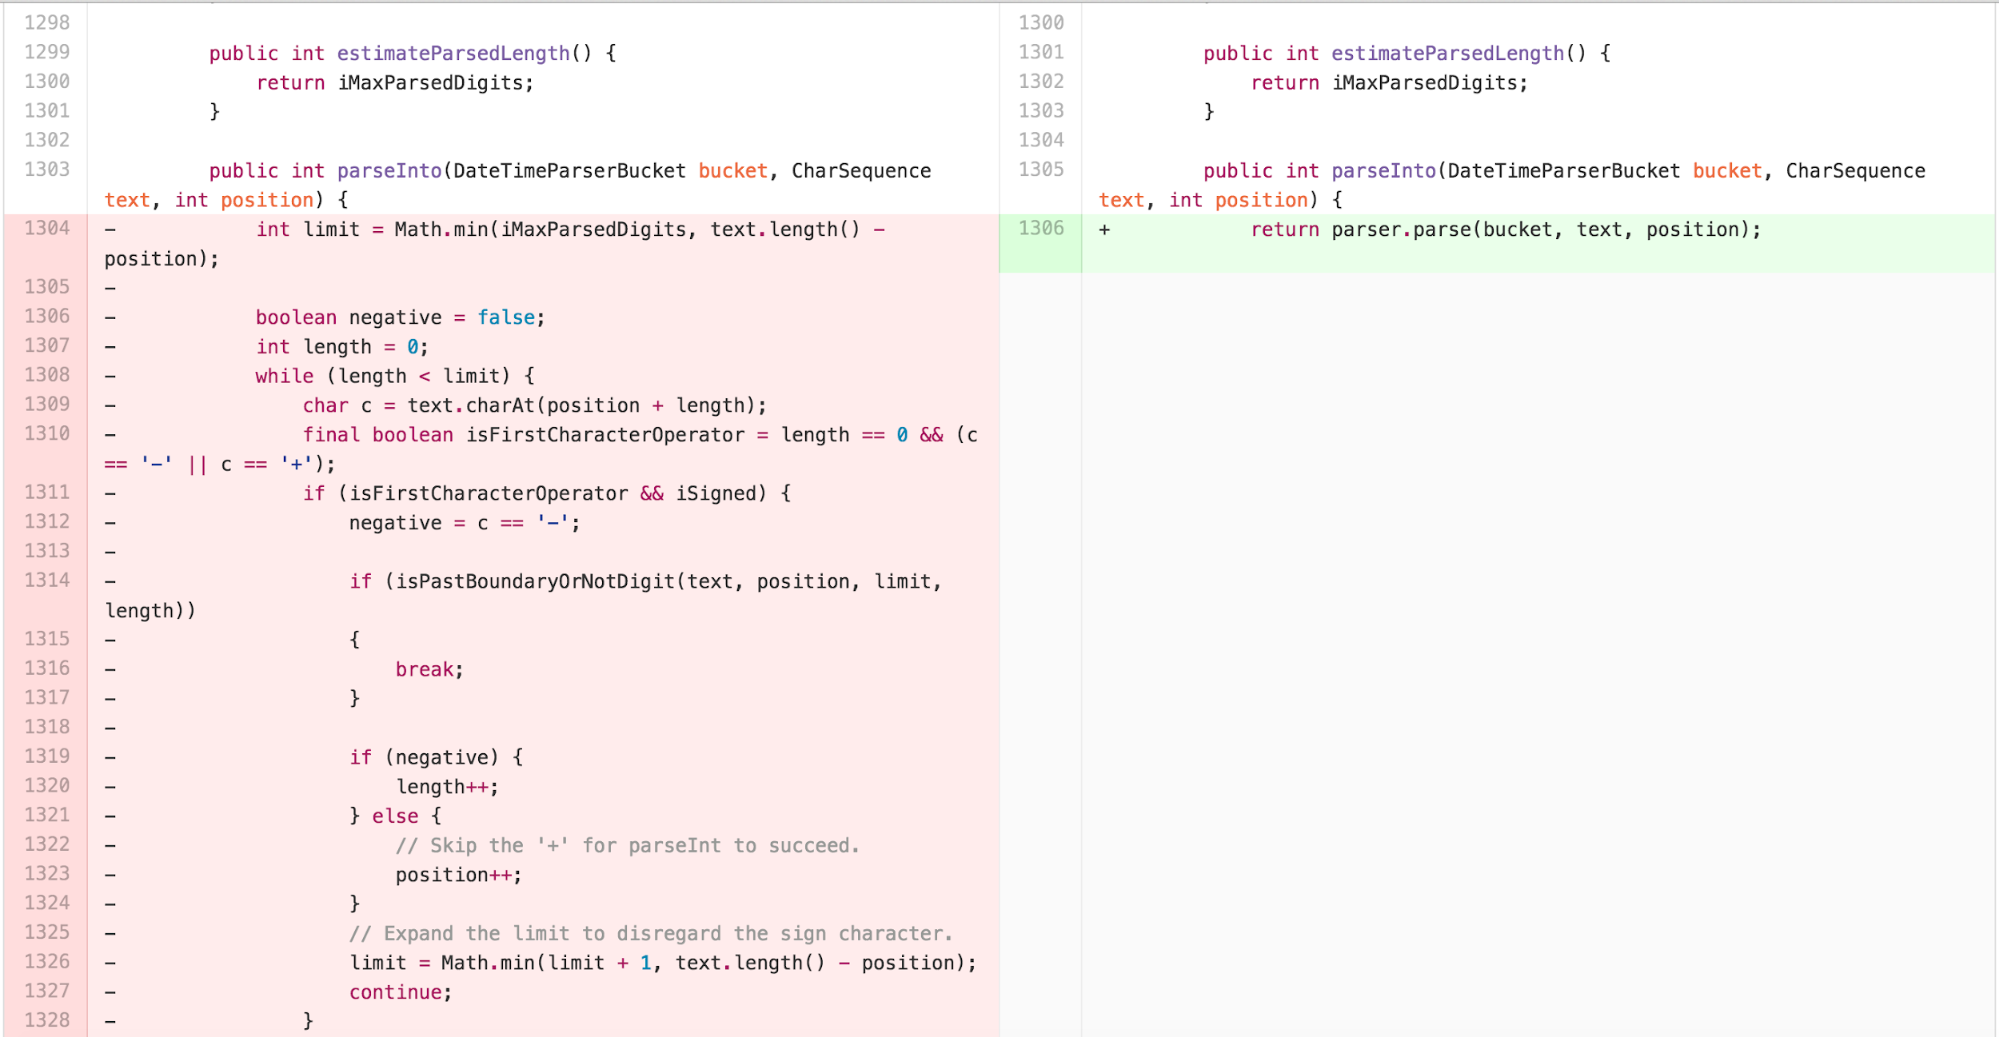
\includegraphics[width=\linewidth]{code6}
	\caption{insert caption}
\end{figure}
\begin{figure}[H]
	\centering
	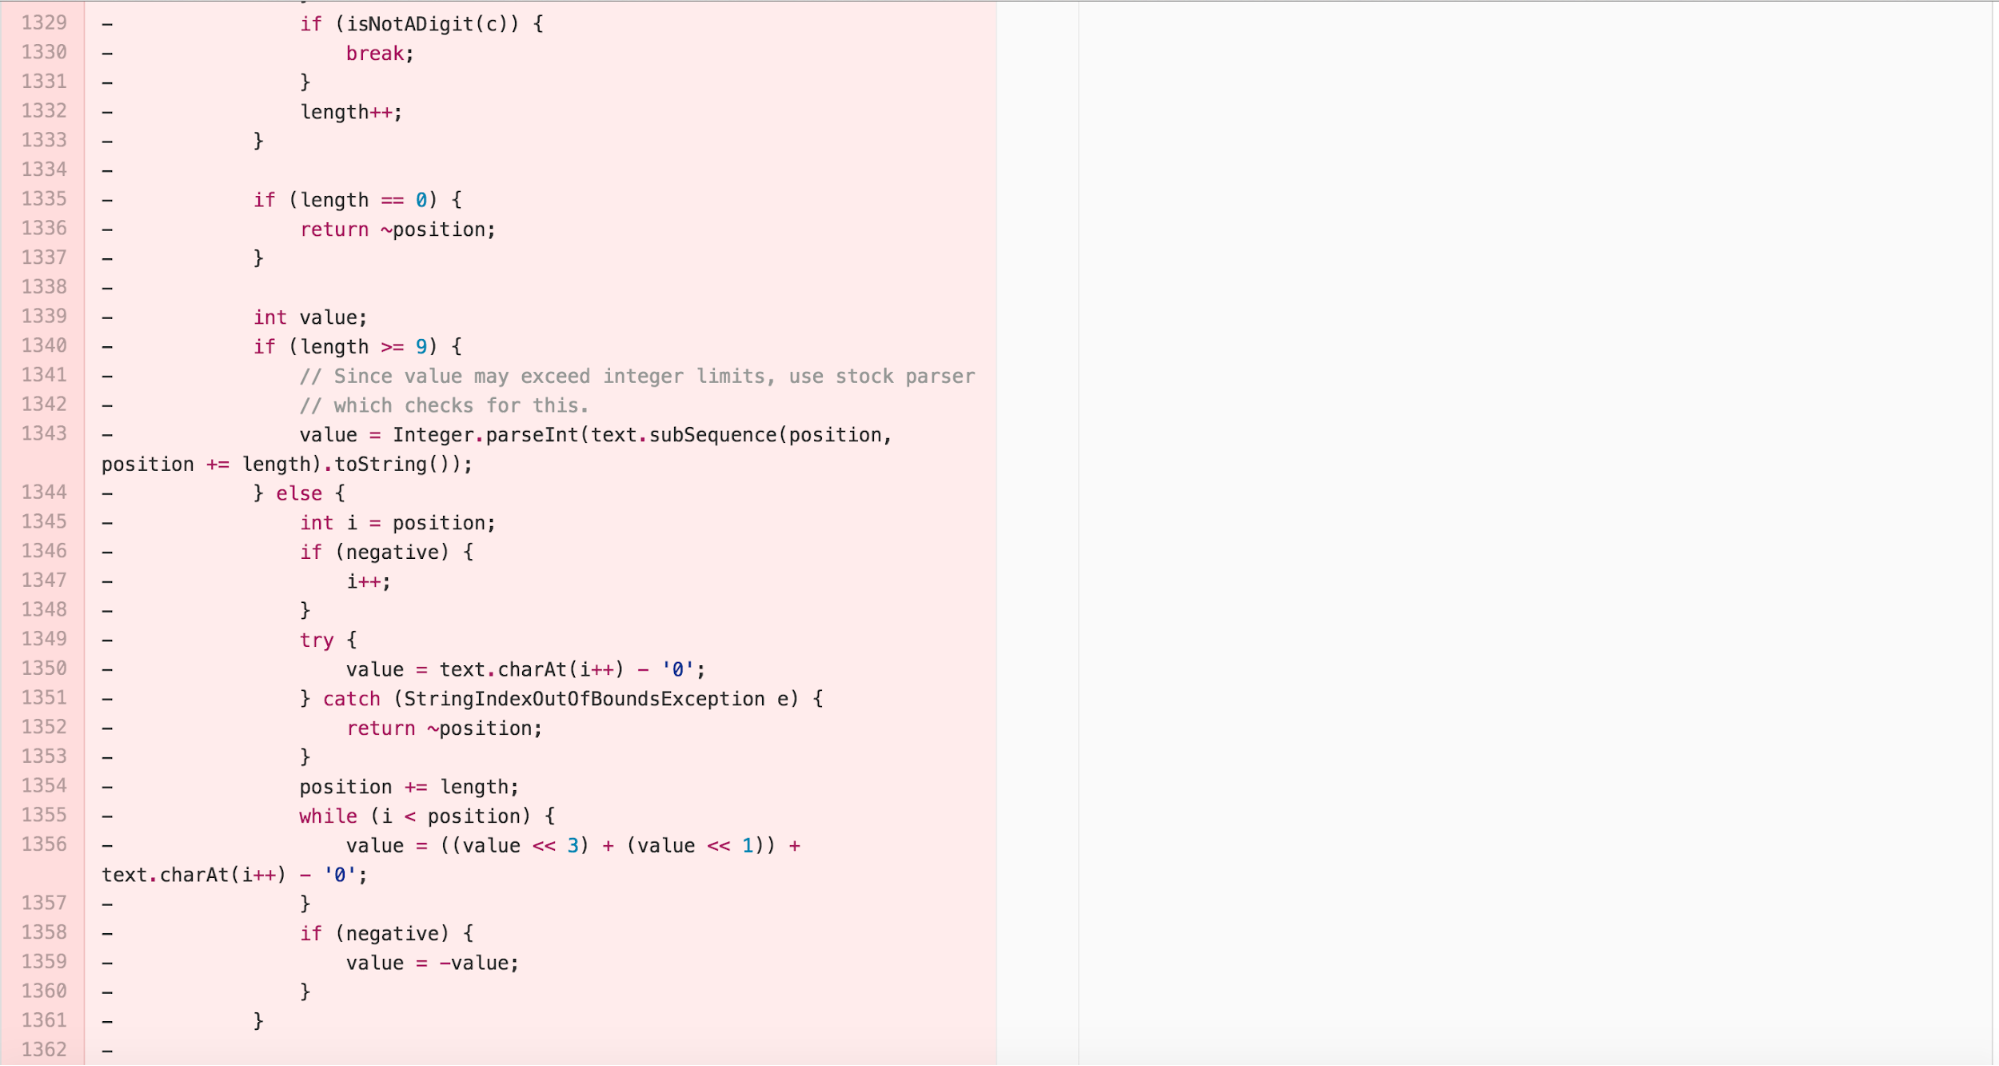
\includegraphics[width=\linewidth]{code7}
	\caption{insert caption}
\end{figure}
\begin{figure}[H]
	\centering
	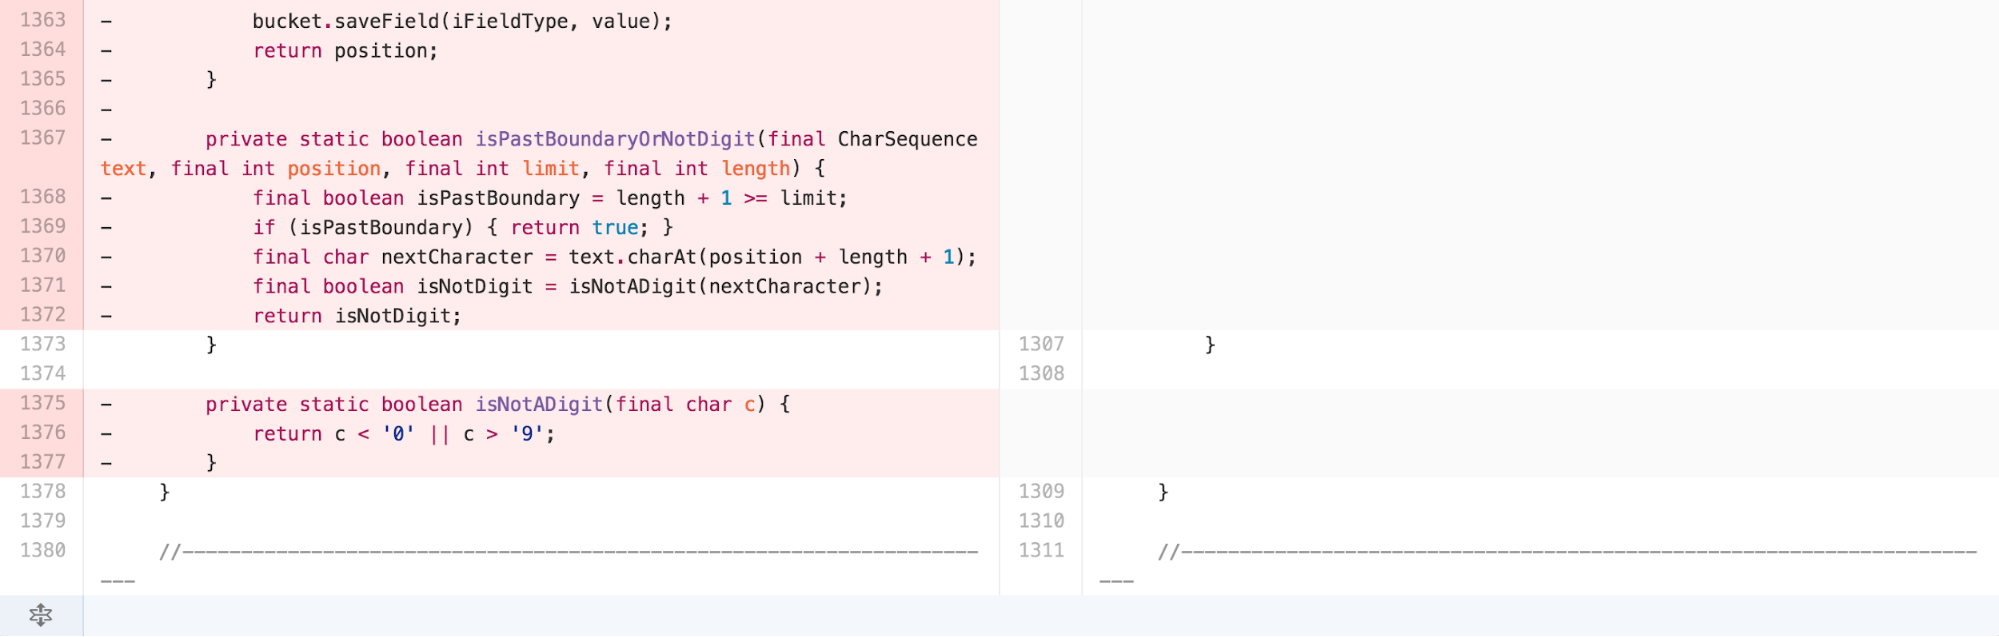
\includegraphics[width=\linewidth]{code8}
	\caption{insert caption}
\end{figure}
\begin{figure}[H]
	\centering
	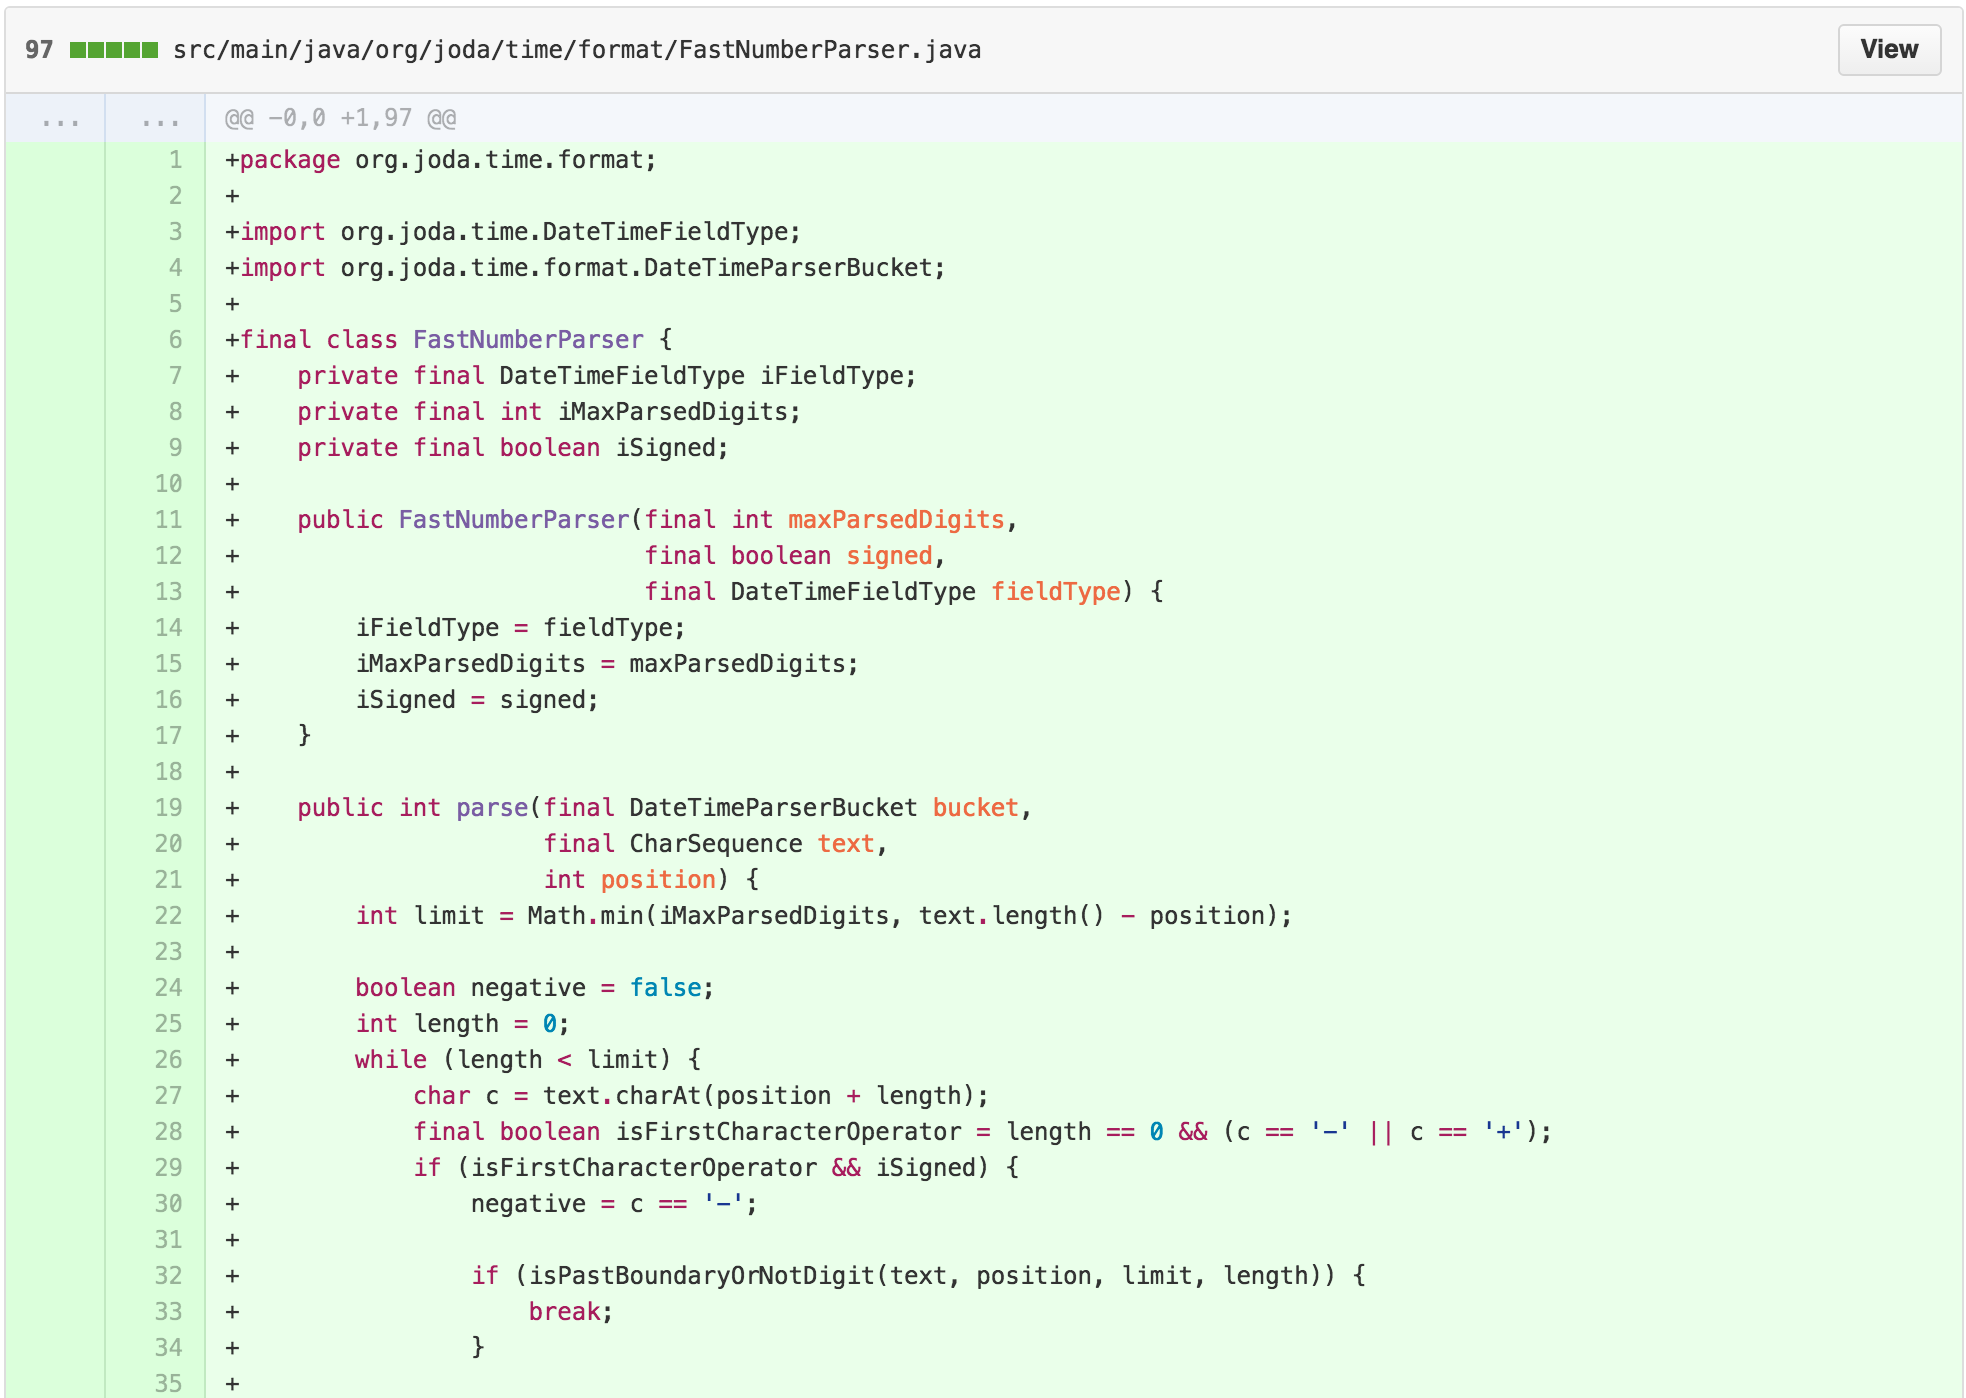
\includegraphics[width=\linewidth]{code9}
	\caption{insert caption}
\end{figure}
\begin{figure}[H]
	\centering
	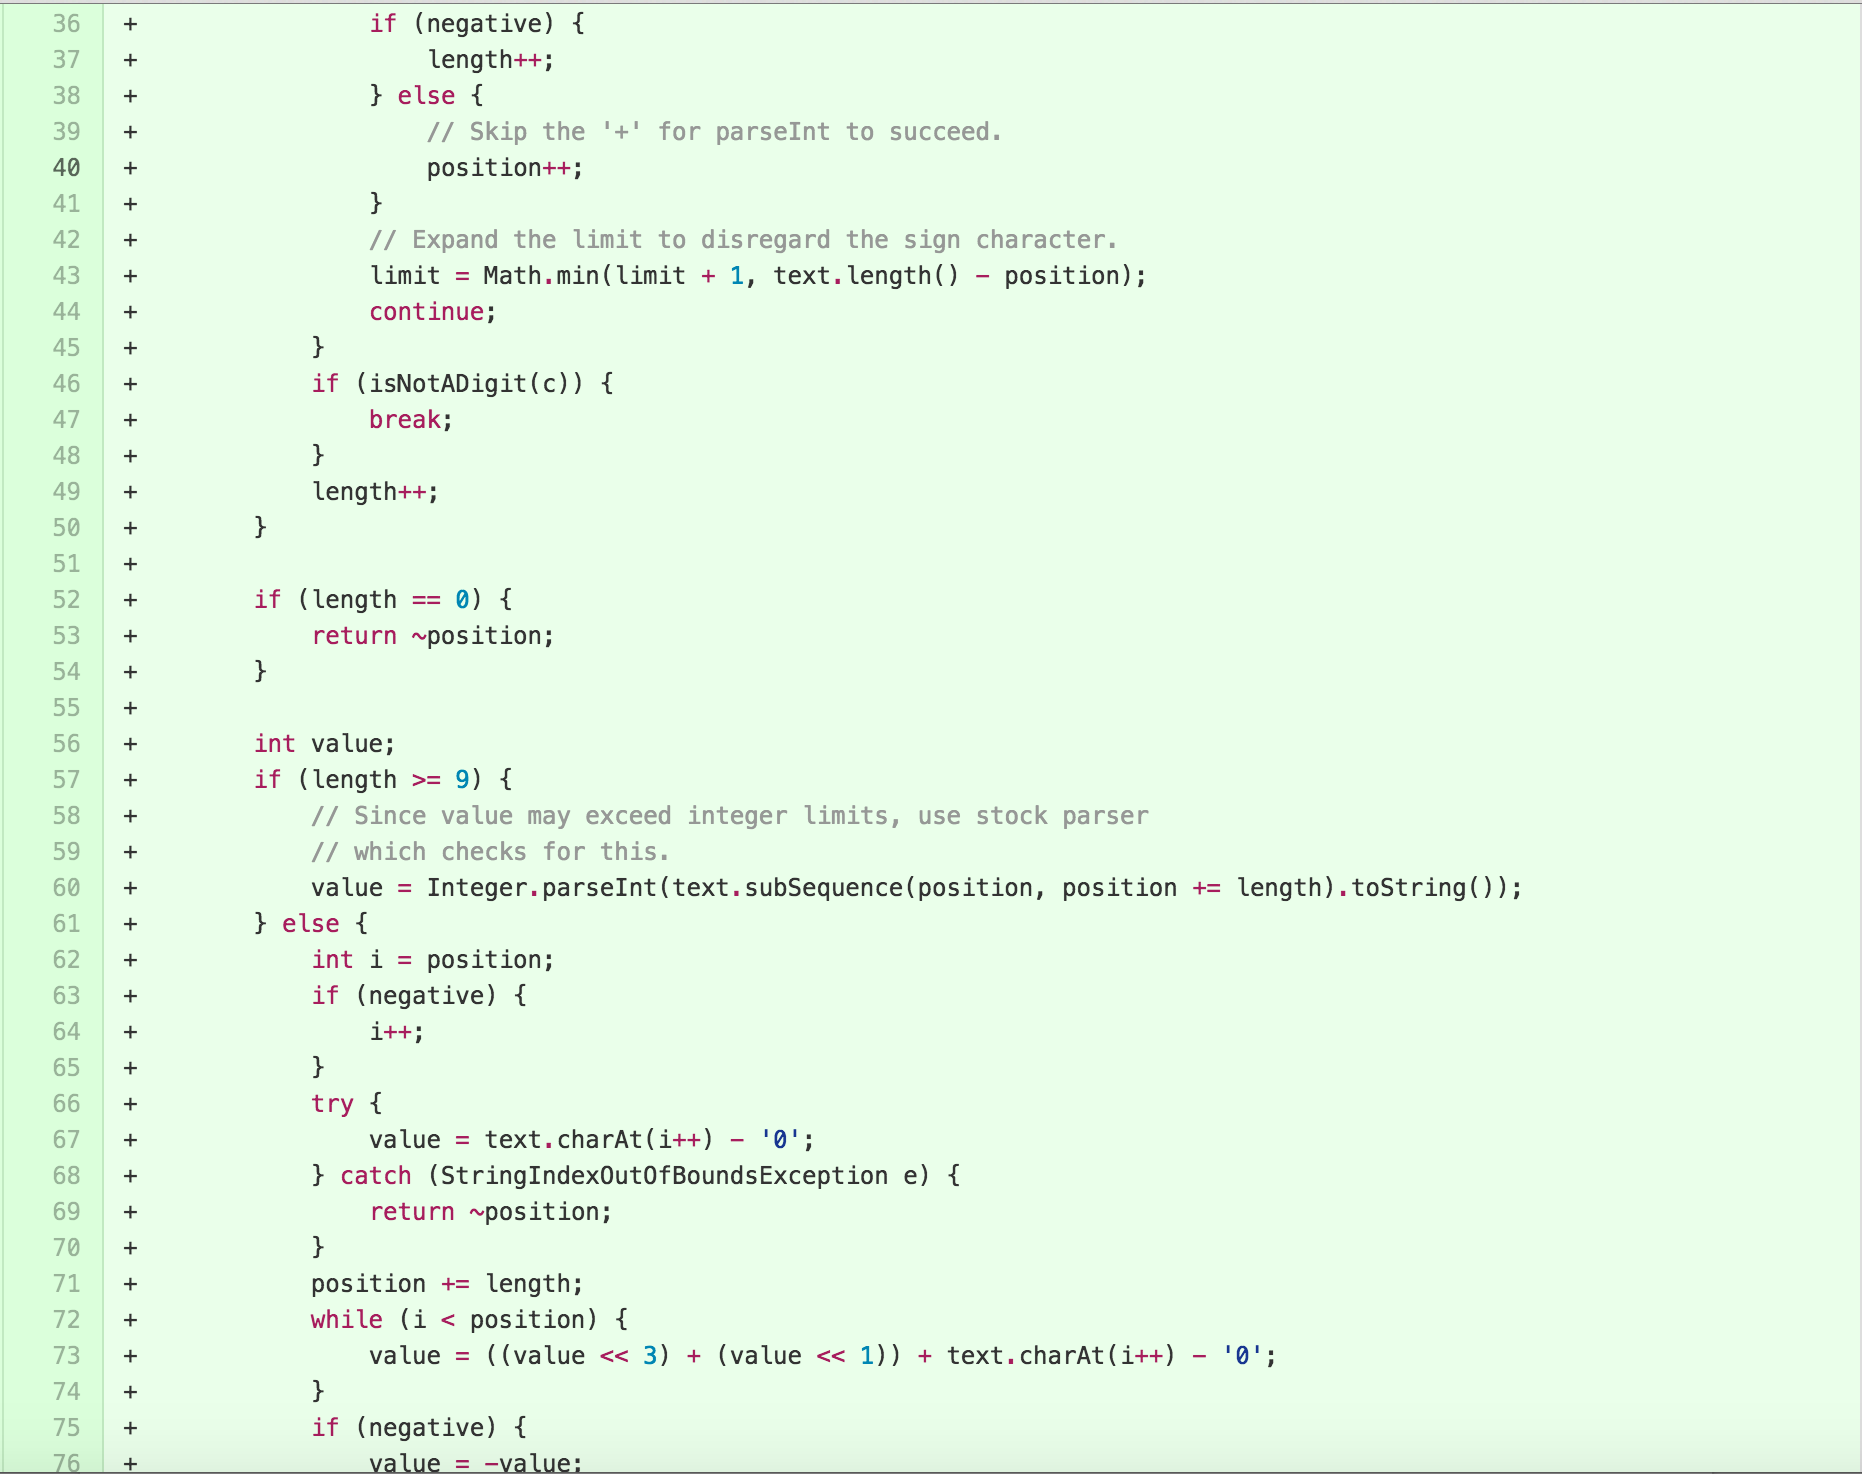
\includegraphics[width=\linewidth]{code10}
	\caption{insert caption}
\end{figure}
\begin{figure}[H]
	\centering
	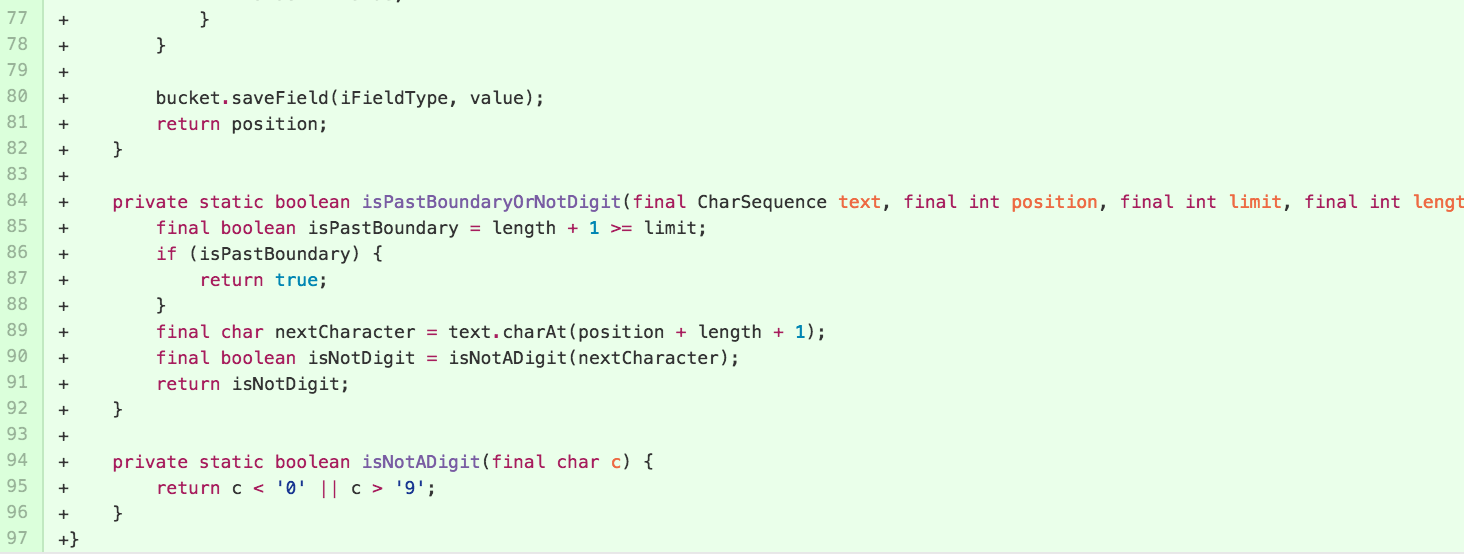
\includegraphics[width=\linewidth]{code11}
	\caption{insert caption}
\end{figure}
The new class is 97 lines long, with the majority of the work happening in the 63 line long \texttt{parse} method. The result of \texttt{parse} can be tested and understood independently of details from the \texttt{NumberFormatter} inside of \texttt{DateTimeFormatterBuilder}.

\section{Reducing Control Flow Complexity}

Some might argue that a 63 line method is “simple enough.”  Working heuristics of working memory, however, suggest that the human brain can fit between 4-9 “chunks” in memory at a particular time. This aligns well with the guidance in Clean Code that “Functions should do One Thing” and “Functions should be small”. Consequently, it’s worth turning attention to simplifying the \texttt{parse} method.

The cognitive complexity of the function is compounded by a variety of control structures. There are 2 while loops, 9 if statements, and 3 return statements. Extracting methods out of such a function is difficult because the multiple control flow breaks and updates to local variables require reasoning that is beyond many static analysis code tools, such as the Refactoring tools in IDEA Intellij. Often it helps to start “from the bottom up”, simplifying small blocks of complicated control structures until the tangled web of control flow clarifies.

First, a little cleanup. I can remove an unused import, as imports add to the cognitive load of a class by signaling interconnection with other components of a system.

\begin{figure}[H]
	\centering
	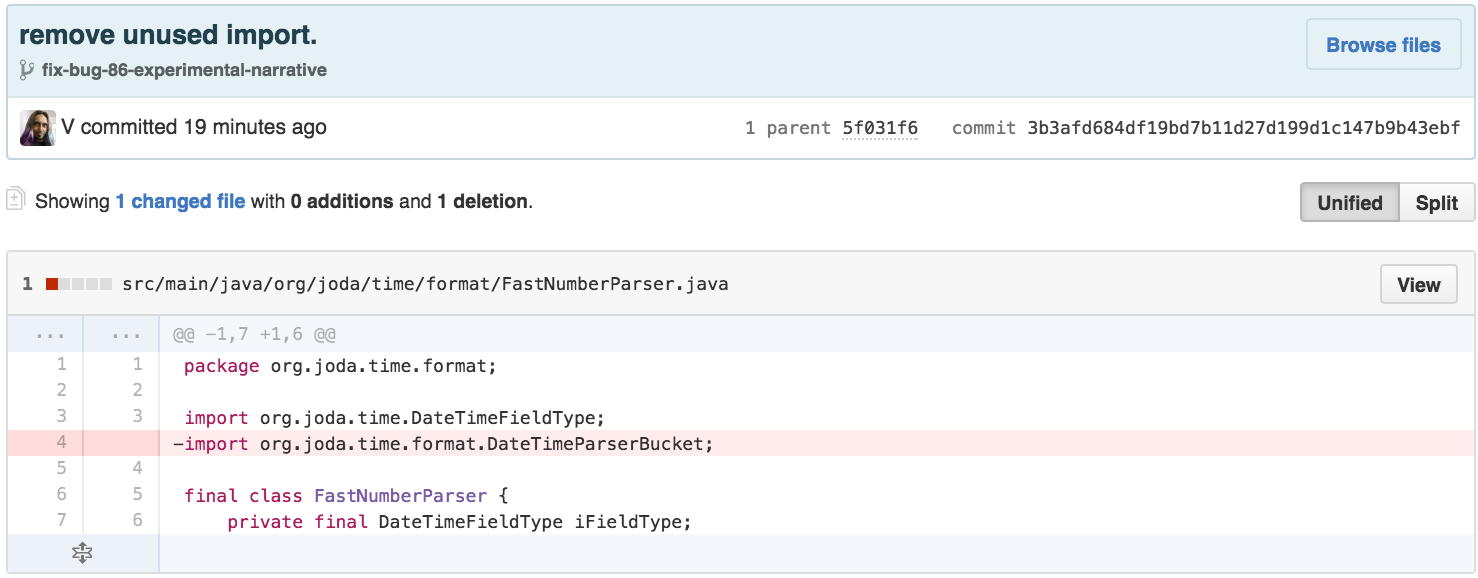
\includegraphics[width=\linewidth]{code12}
	\caption{insert caption}
\end{figure}

Next, I simplify according to the Principle of Least Astonishment by replacing the use of a StringIndexOutOfBoundsException for flow control (commonly argued in the literature) with a GUARD CLAUSE.

\begin{figure}[H]
	\centering
	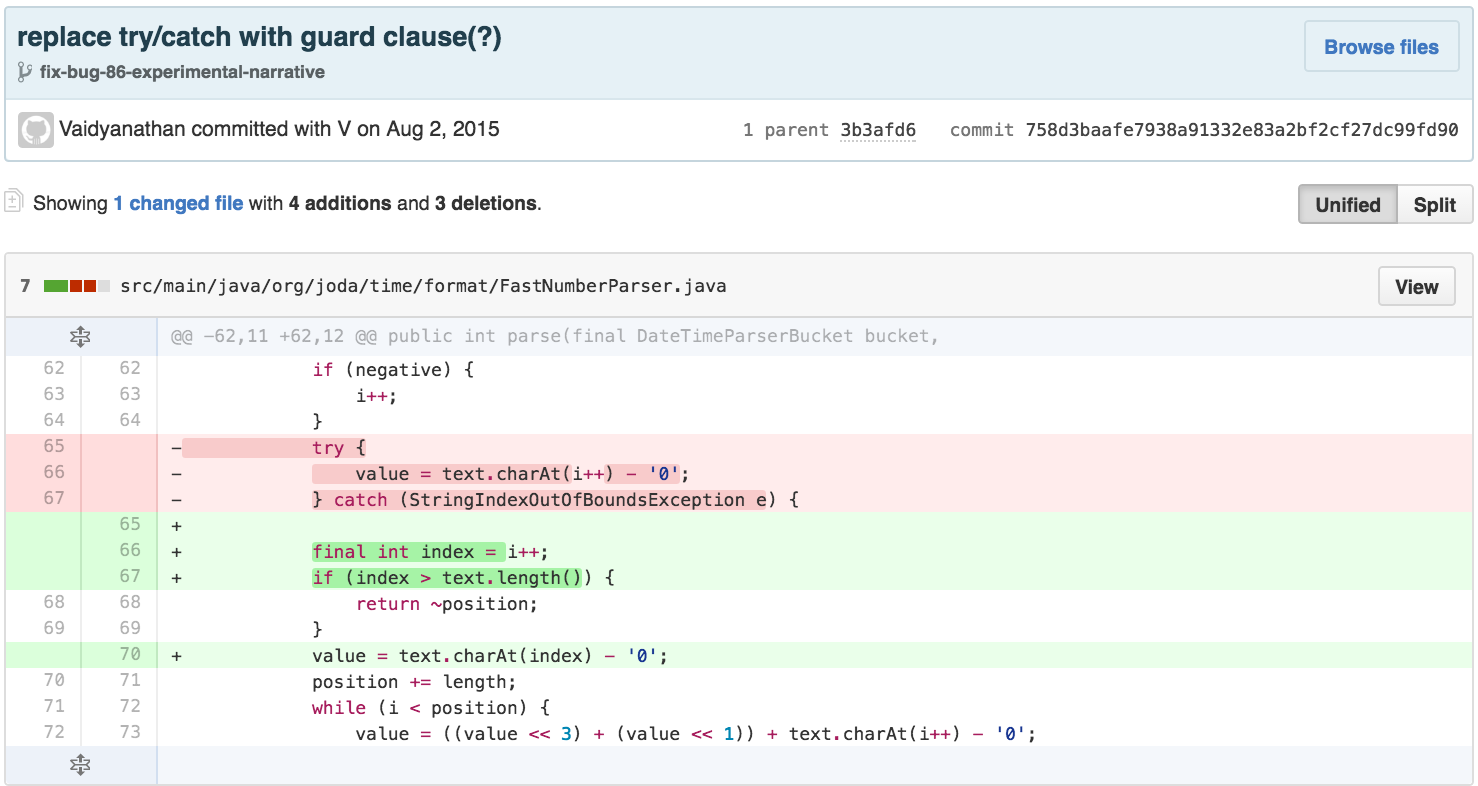
\includegraphics[width=\linewidth]{code13}
	\caption{insert caption}
\end{figure}


The body of \texttt{parse} has a strong visual indicator of separation between the first while loop, which updates the \texttt{position} and \texttt{length} variables, and a second “section” that calculates the value. In order to be able to break out methods effectively, I want to simplify the control flow of each.

Examining the body of the while loop, I see that it basically increments \texttt{length} every iteration. It breaks out of the loop if the current character is not a digit, and applies some special case updates if the first character is an operator and the parser knows the input contains one. I can simplify the special casing using explanatory variables and use REPLACE NESTED CONDITIONALS WITH GUARD CLAUSES to reduce the number of nested scopes. I also changed the previously extracted method \texttt{isPastBoundaryOrNotDigit} - -which by its very name does more than 1 thing-- into 2 separate methods that are invoked by the caller.

\begin{figure}[H]
	\centering
	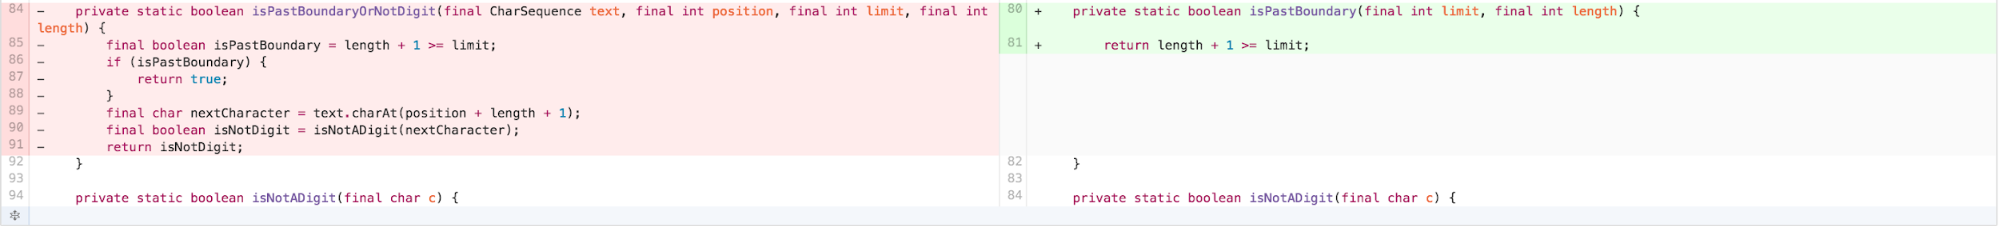
\includegraphics[width=\linewidth]{code14}
	\caption{insert caption}
\end{figure}
\begin{figure}[H]
	\centering
	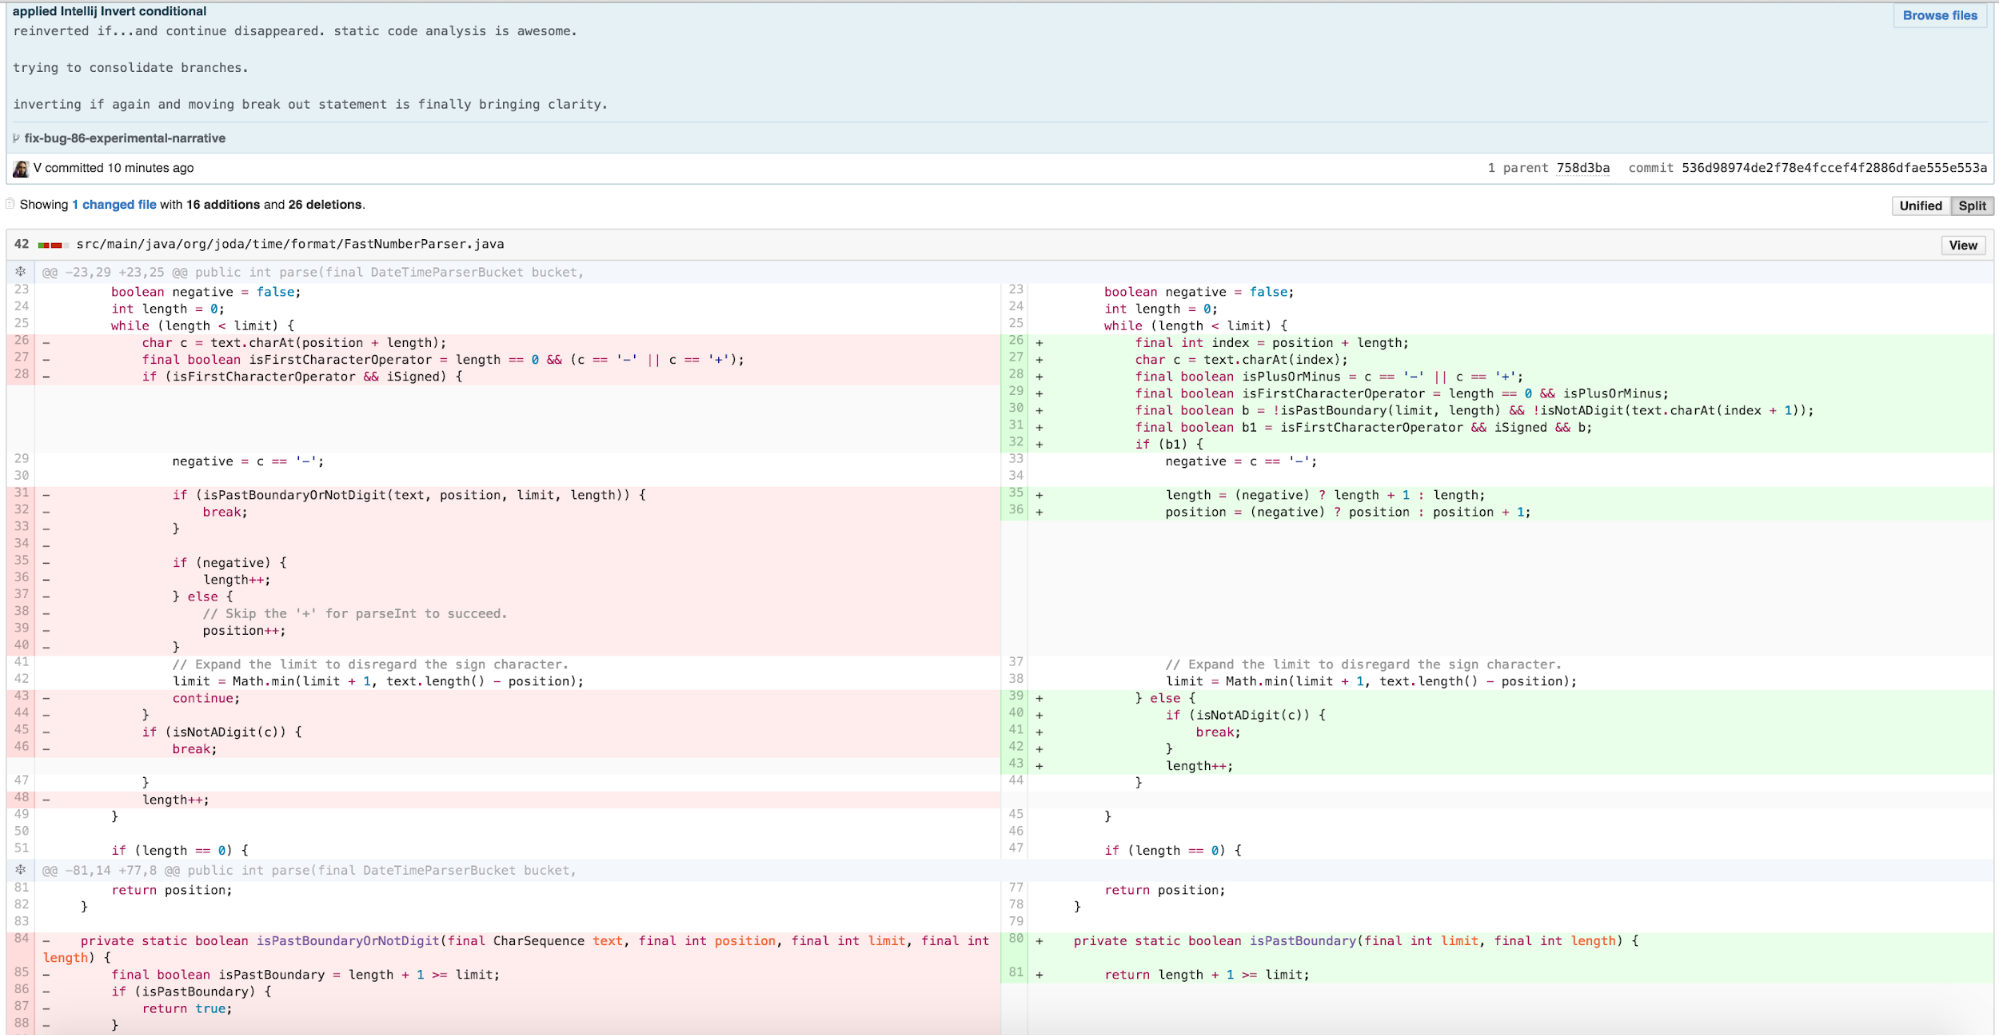
\includegraphics[width=\linewidth]{code15}
	\caption{insert caption}
\end{figure}

Seeking to further simplify the remaining \texttt{if/else} block inside the body of the \texttt{while}, I looked carefully at the special case logic for an operator and the \texttt{else} body and determined that both code paths incremented \texttt{length}. This type of conditional check to do the same thing in both cases is clearly extraneous cognitive load, so I applied a variant of CONSOLIDATE CONDITIONAL EXPRESSION.

\begin{figure}[H]
	\centering
	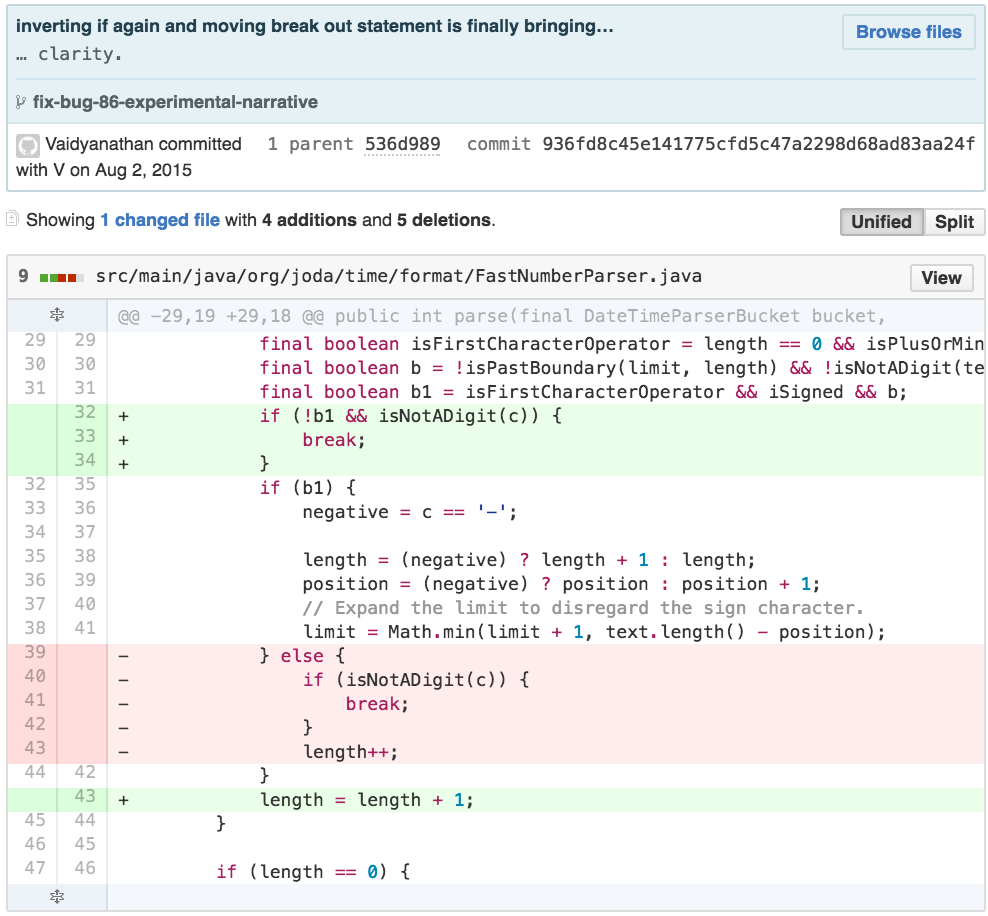
\includegraphics[width=\linewidth]{code16}
	\caption{insert caption}
\end{figure}

I then had an opportunity to simplify the while loop further by applying a similar procedure to a variant of REMOVE CONTROL FLAG to remove the break statement and clarify the loop predicate.

\begin{figure}[H]
	\centering
	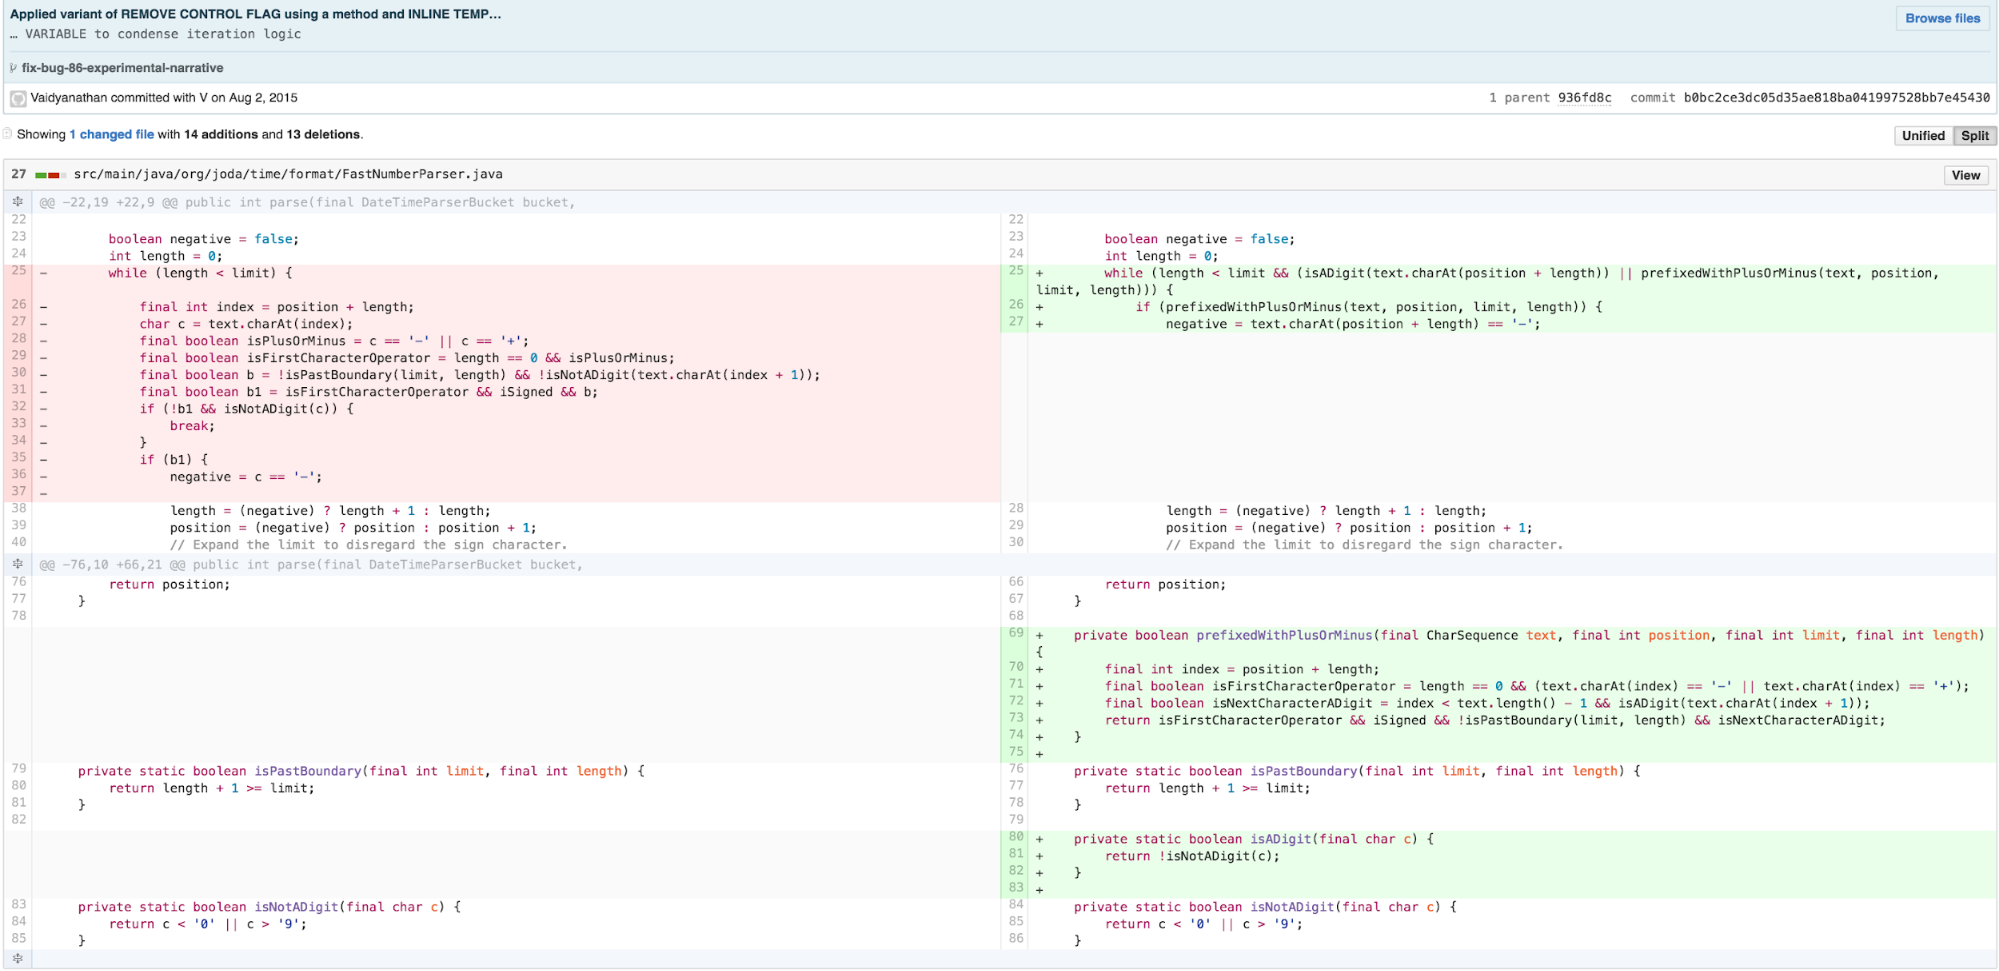
\includegraphics[width=\linewidth]{code17}
	\caption{insert caption}
\end{figure}

With this logic greatly simplified, I’m now able to push the calculation into a smaller, more cohesive chunk of logic using REPLACE METHOD WITH METHOD OBJECT.

\begin{figure}[H]
	\centering
	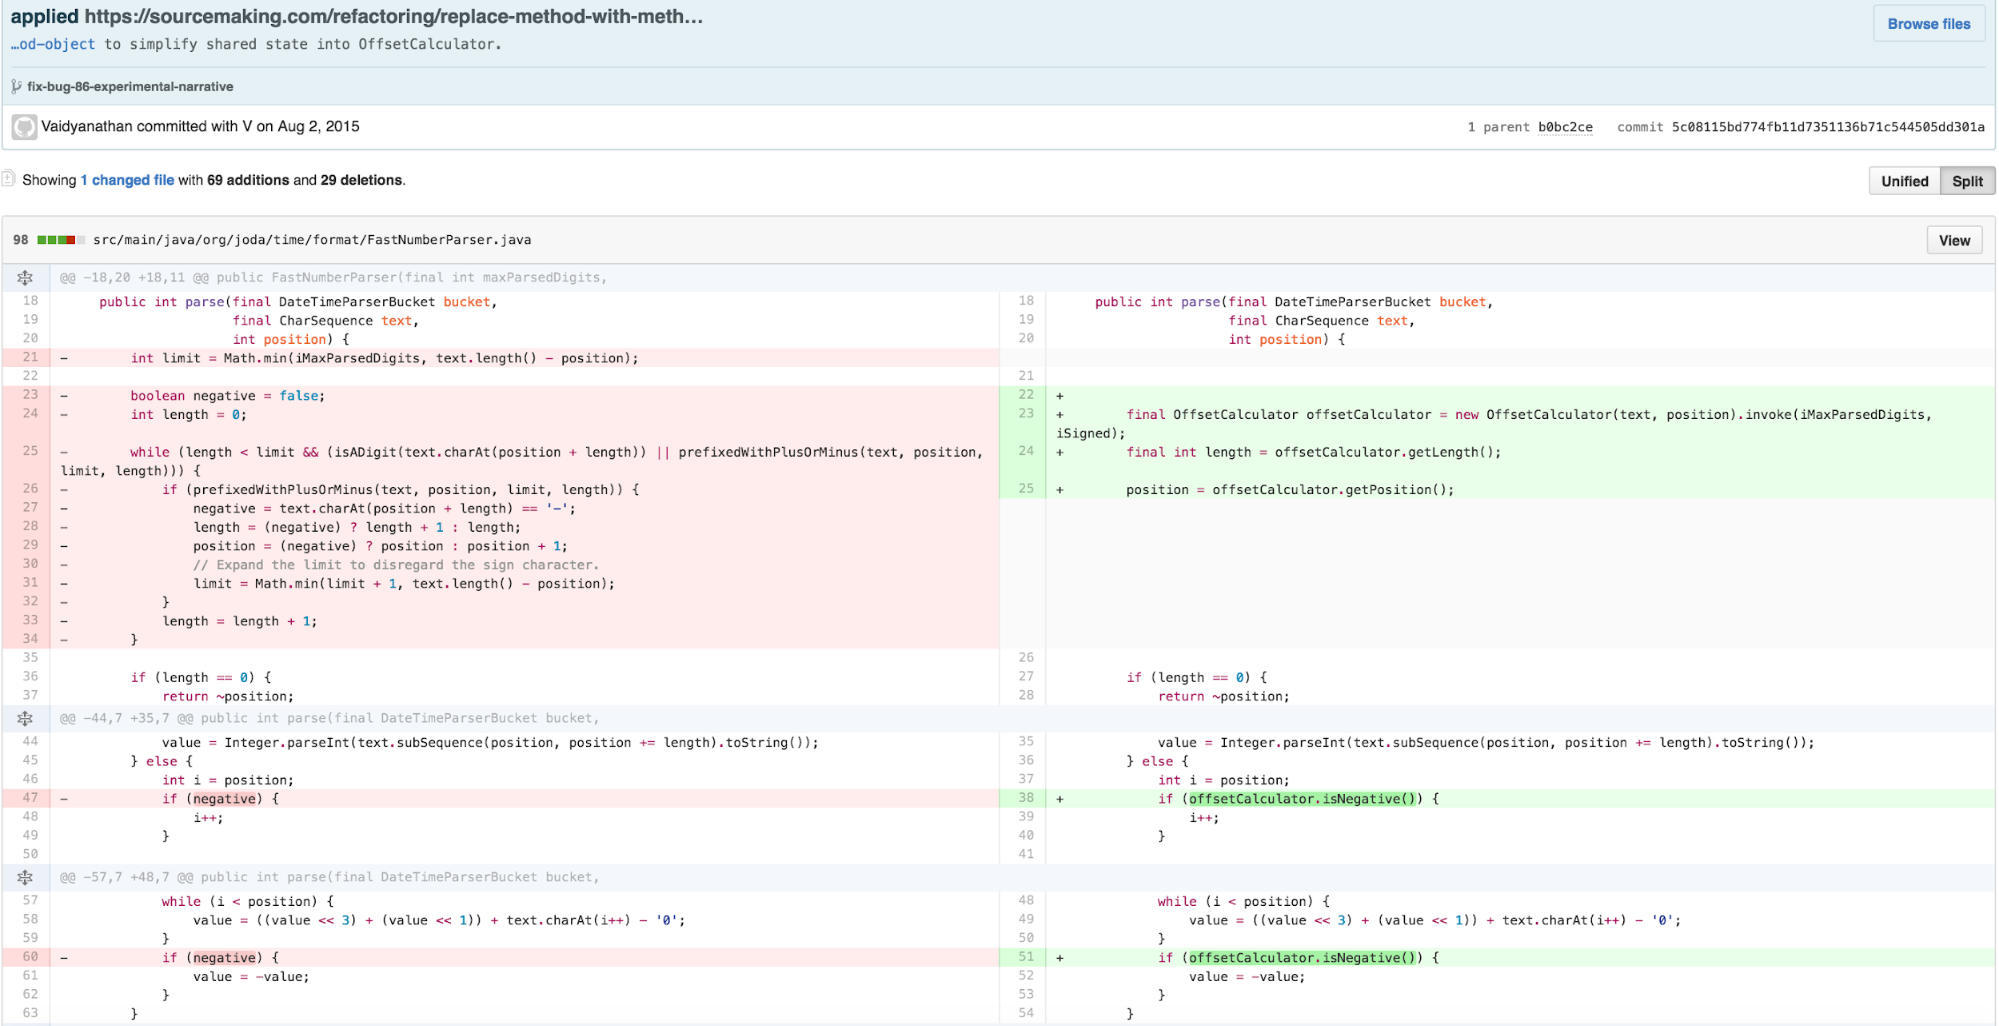
\includegraphics[width=\linewidth]{code18}
	\caption{insert caption}
\end{figure}
\begin{figure}[H]
	\centering
	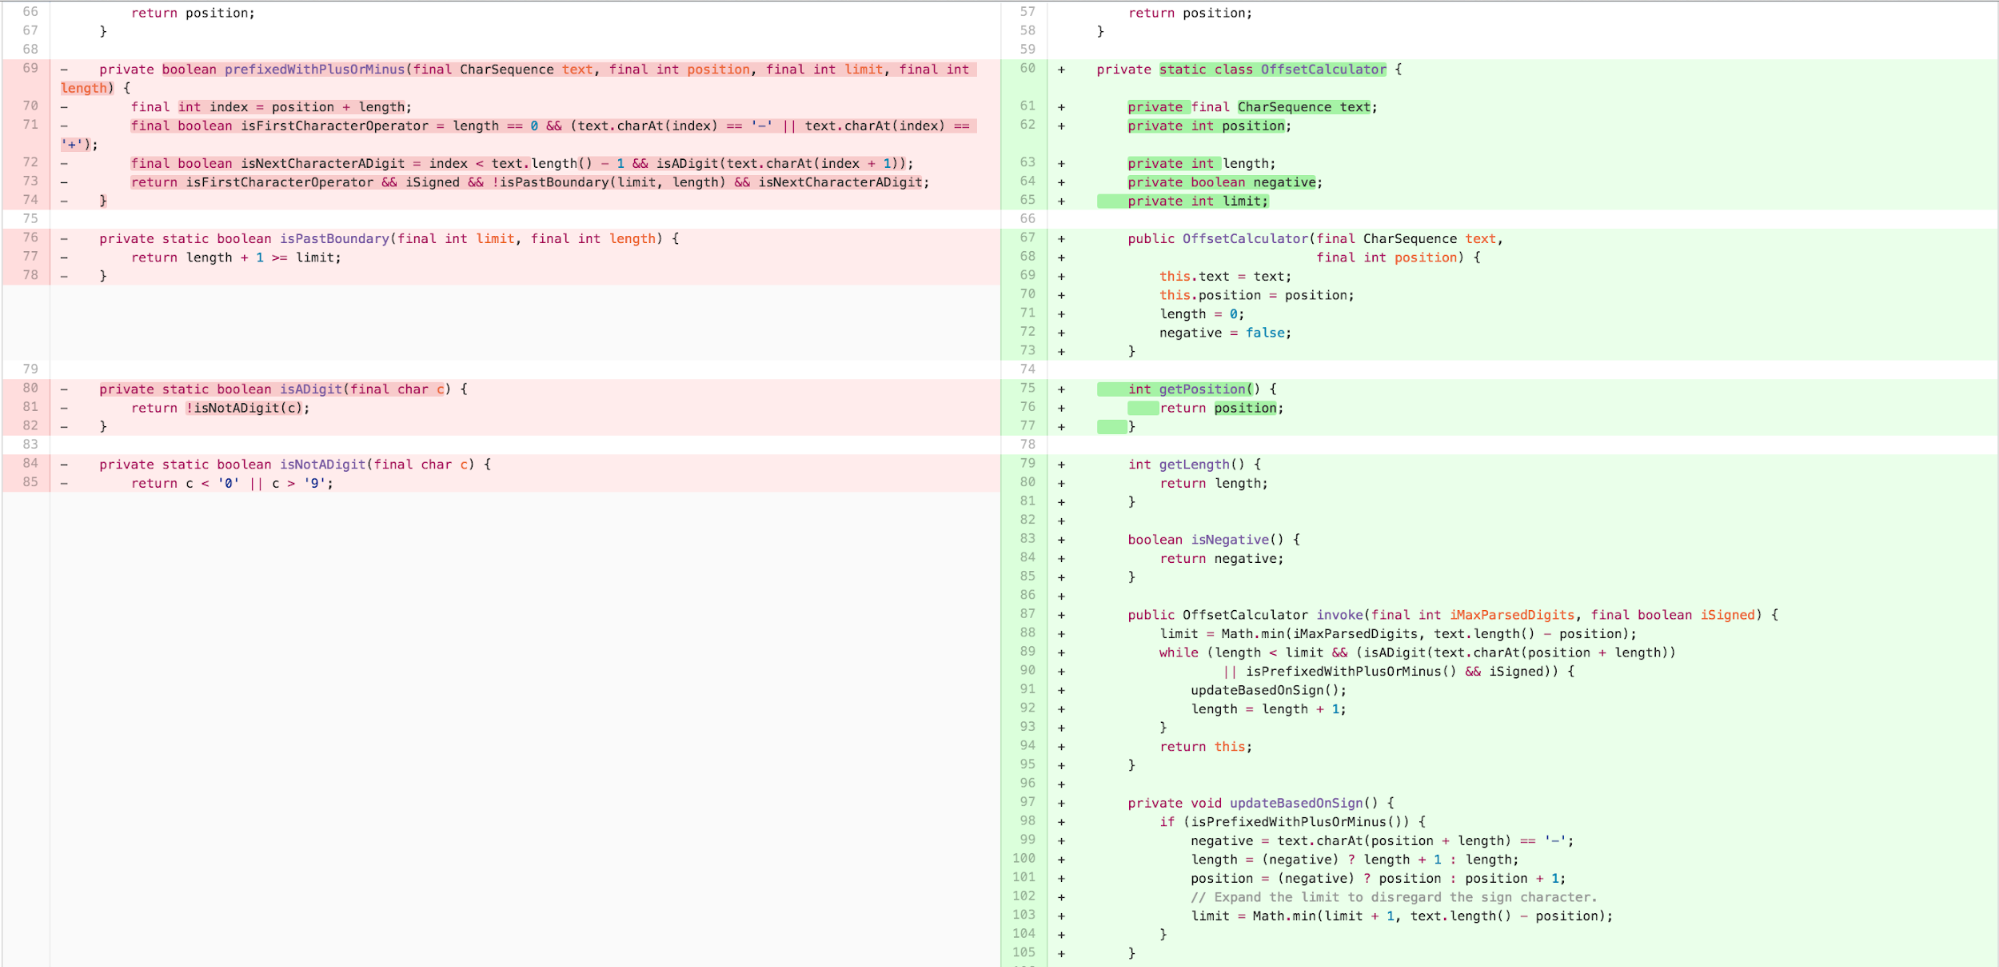
\includegraphics[width=\linewidth]{code19}
	\caption{insert caption}
\end{figure}
\begin{figure}[H]
	\centering
	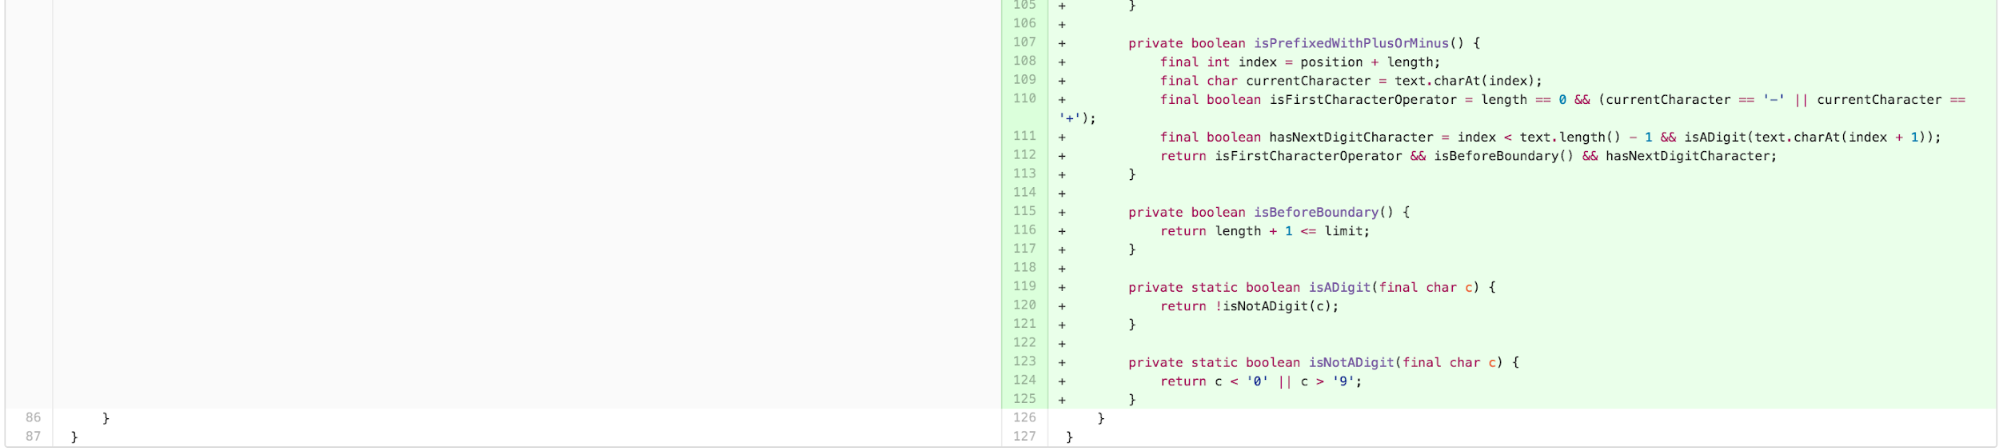
\includegraphics[width=\linewidth]{code20}
	\caption{insert caption}
\end{figure}
Next I wanted to ensure that the new class was inline with CLT’s guidance on sequencing content effectively for comprehension, in line with the recommendations of Clean Code’s STEPDOWN RULE/The Newspaper Metaphor.

\begin{figure}[H]
	\centering
	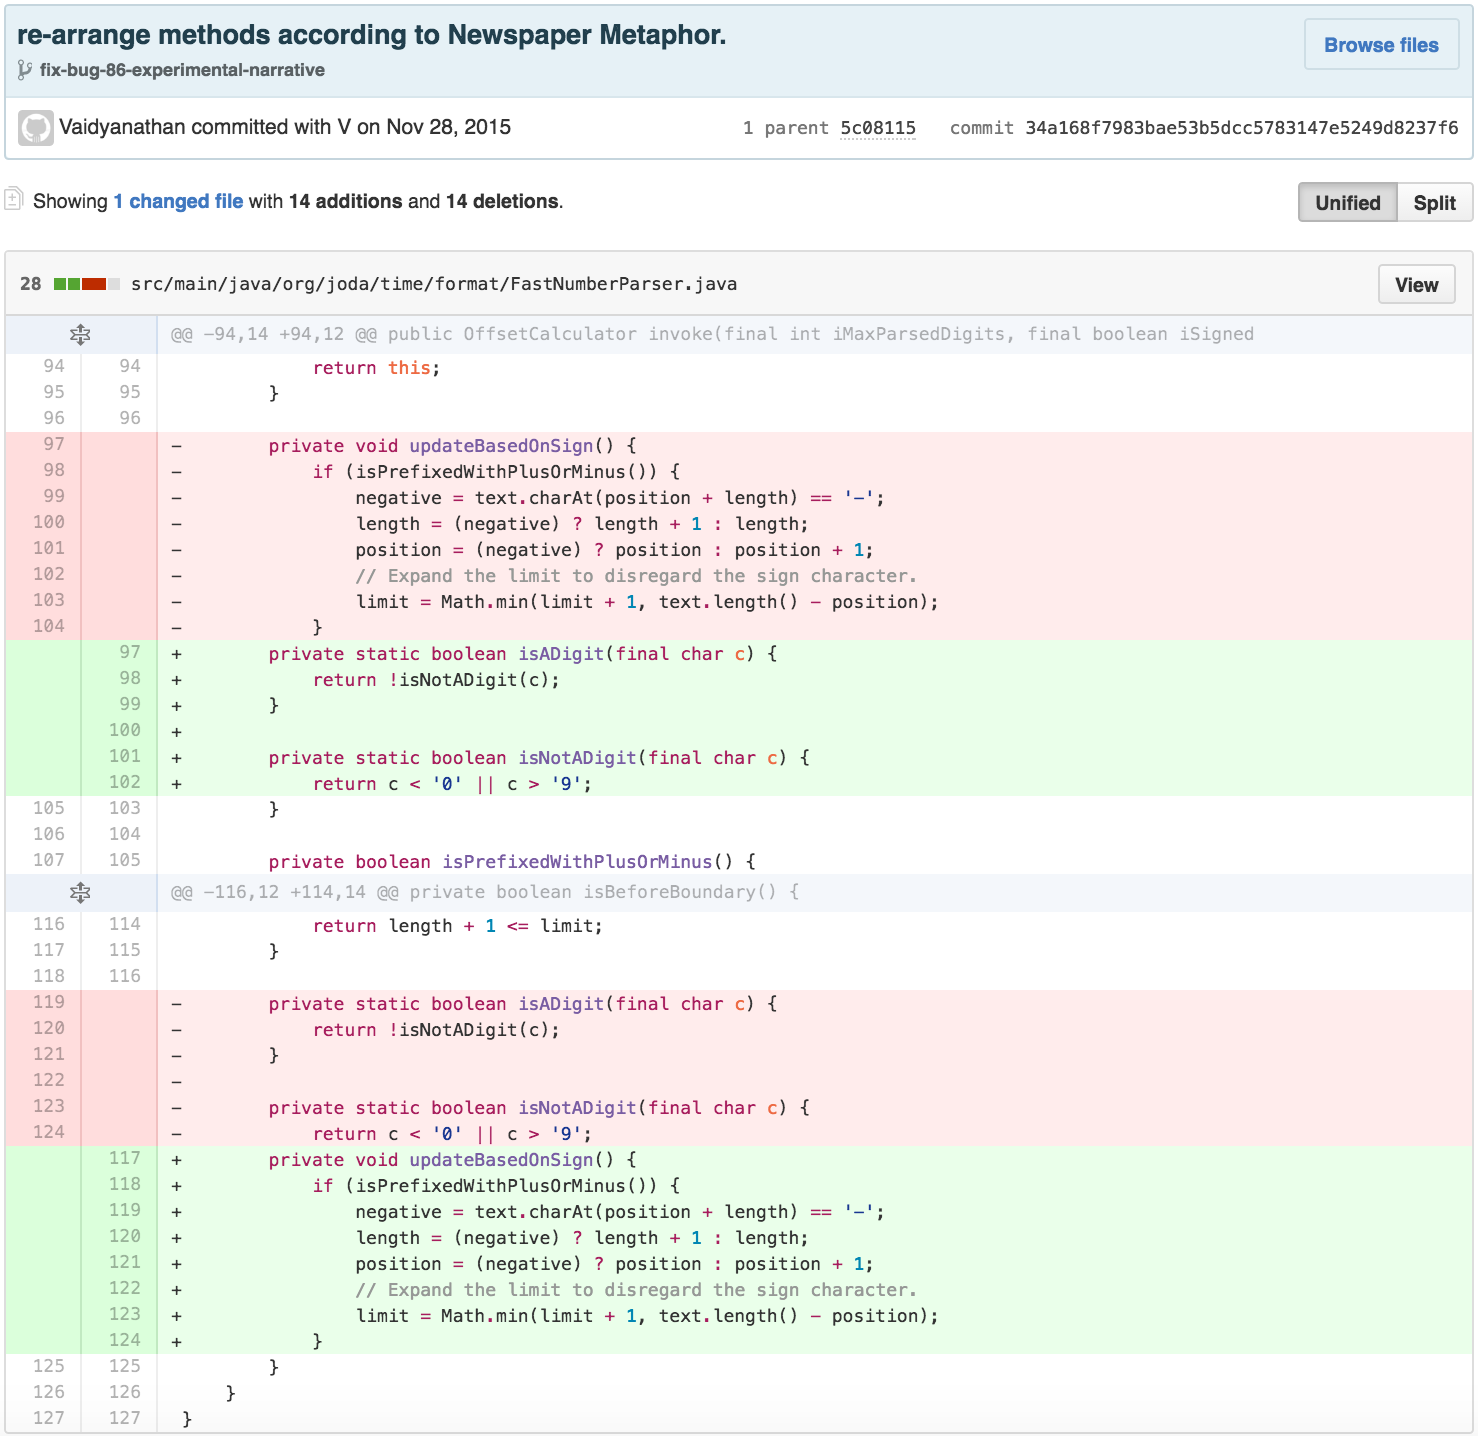
\includegraphics[width=\linewidth]{code21}
	\caption{insert caption}
\end{figure}

The new structure of the parse code had successfully dealt with the length and position calculation loop, but still had 35 lines. Much of the next body of work was involved in calculating a value with the stored computed values of \texttt{OffsetCalculator}. While this type of code practice is common, and the resulting \texttt{OffsetCalculator} is arguably much simpler, it violates the Tell, Don’t Ask principle of object-oriented programming. Tell, Don’t Ask helps manage the intrinsic cognitive load of systems by pushing operations on data closer to the data, making code more declarative. Following this approach, we move the value calculation into the \texttt{OffsetCalculator} and eliminate \texttt{FastNumberParser}.

\begin{figure}[H]
	\centering
	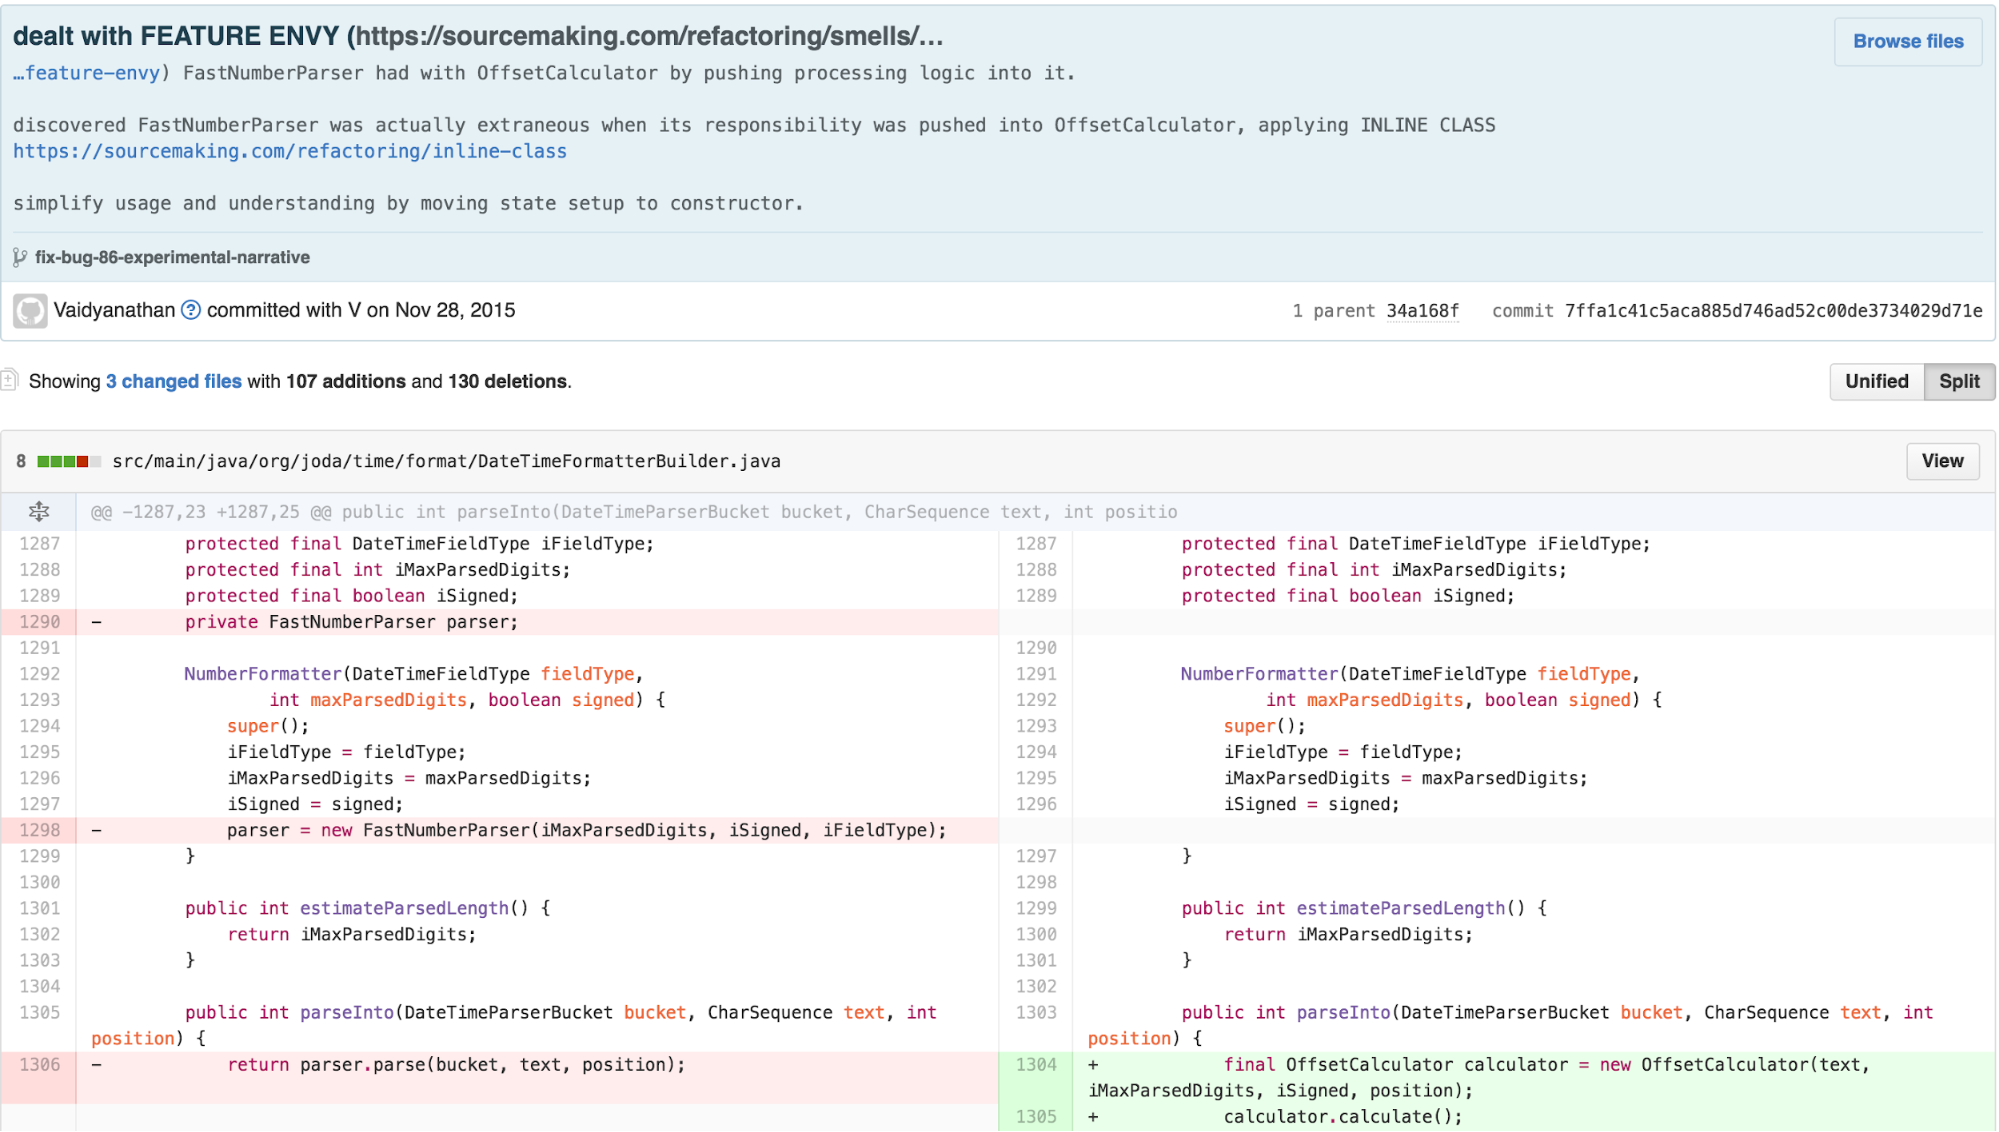
\includegraphics[width=\linewidth]{code22}
	\caption{insert caption}
\end{figure}
\begin{figure}[H]
	\centering
	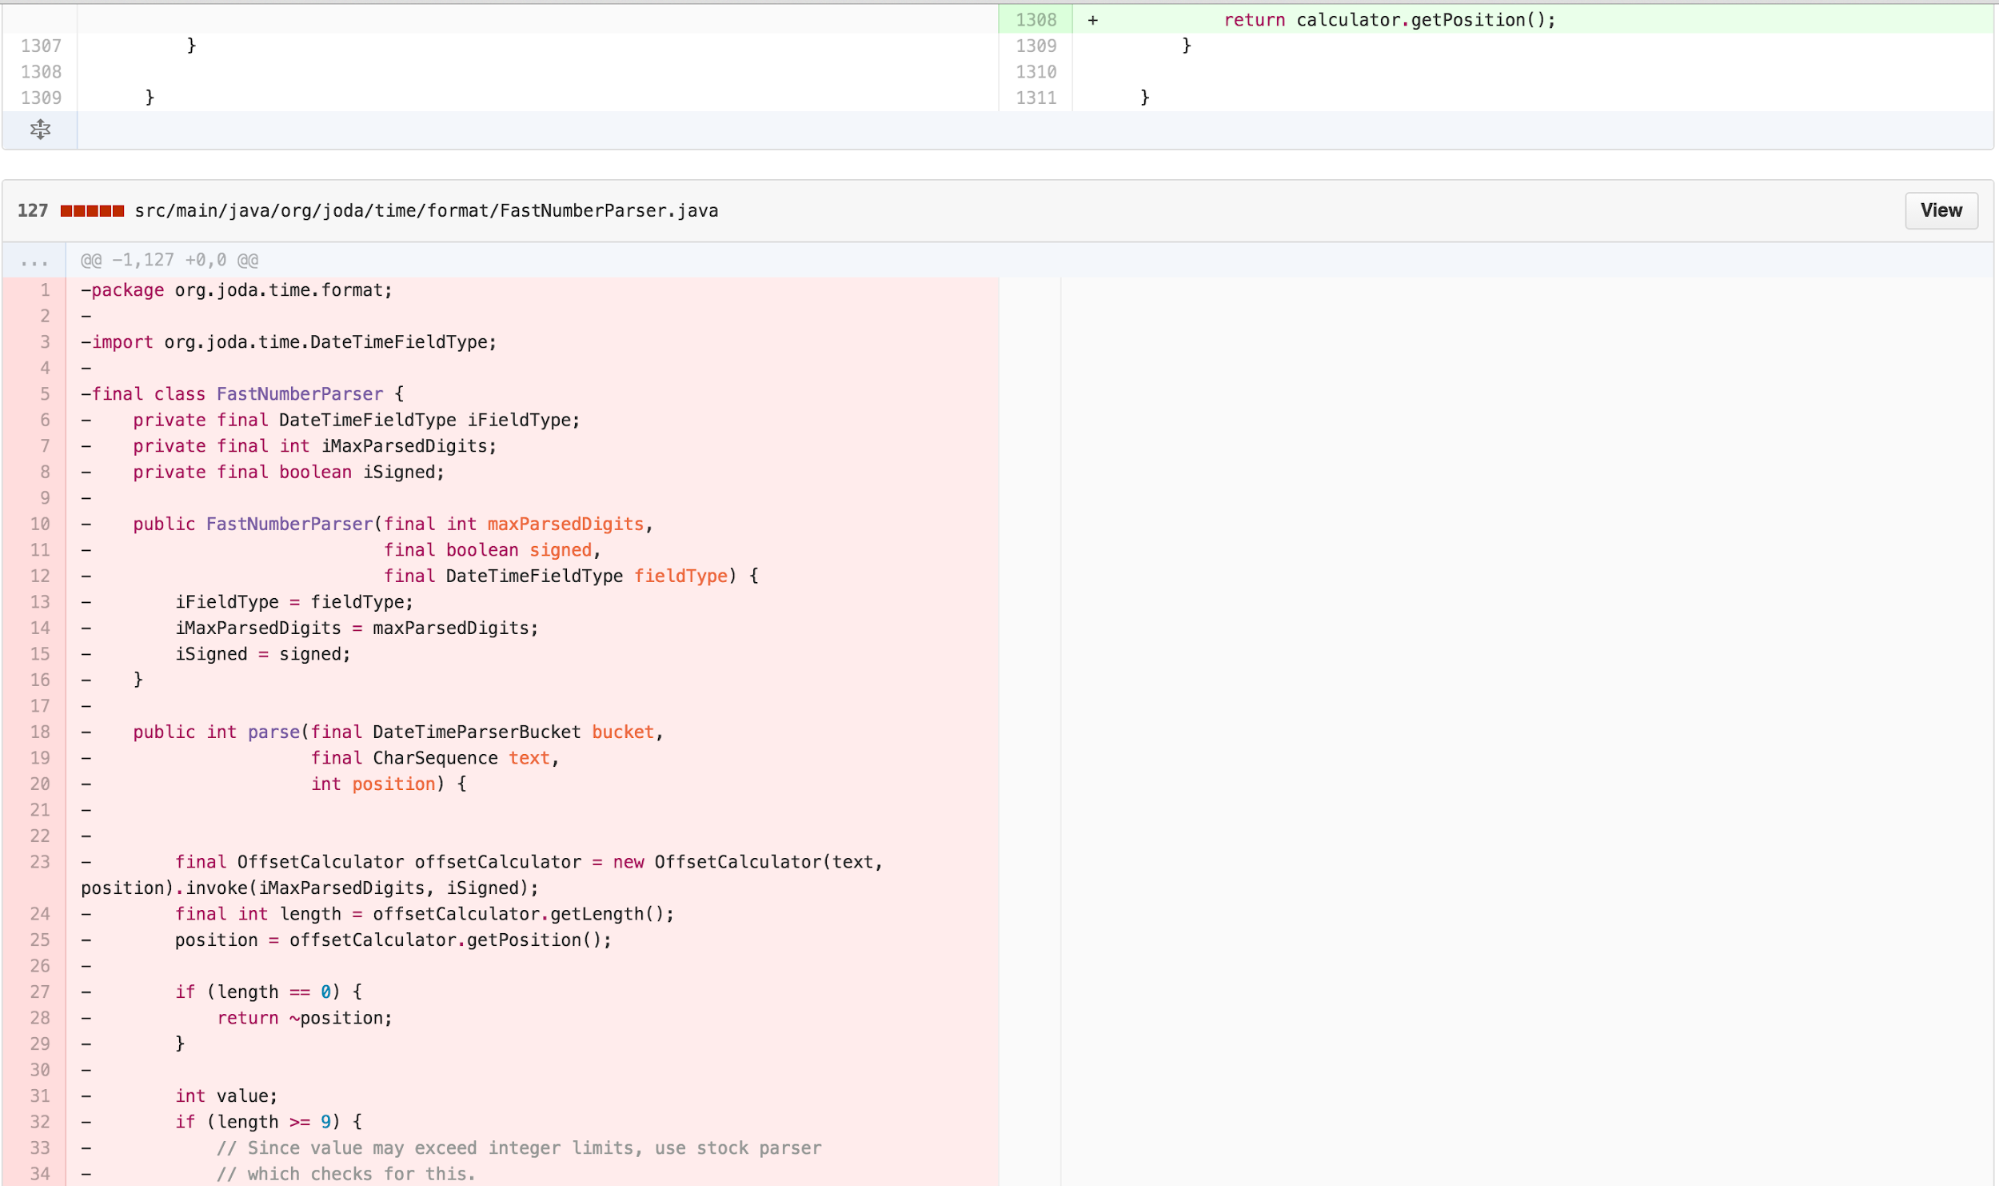
\includegraphics[width=\linewidth]{code23}
	\caption{insert caption}
\end{figure}
\begin{figure}[H]
	\centering
	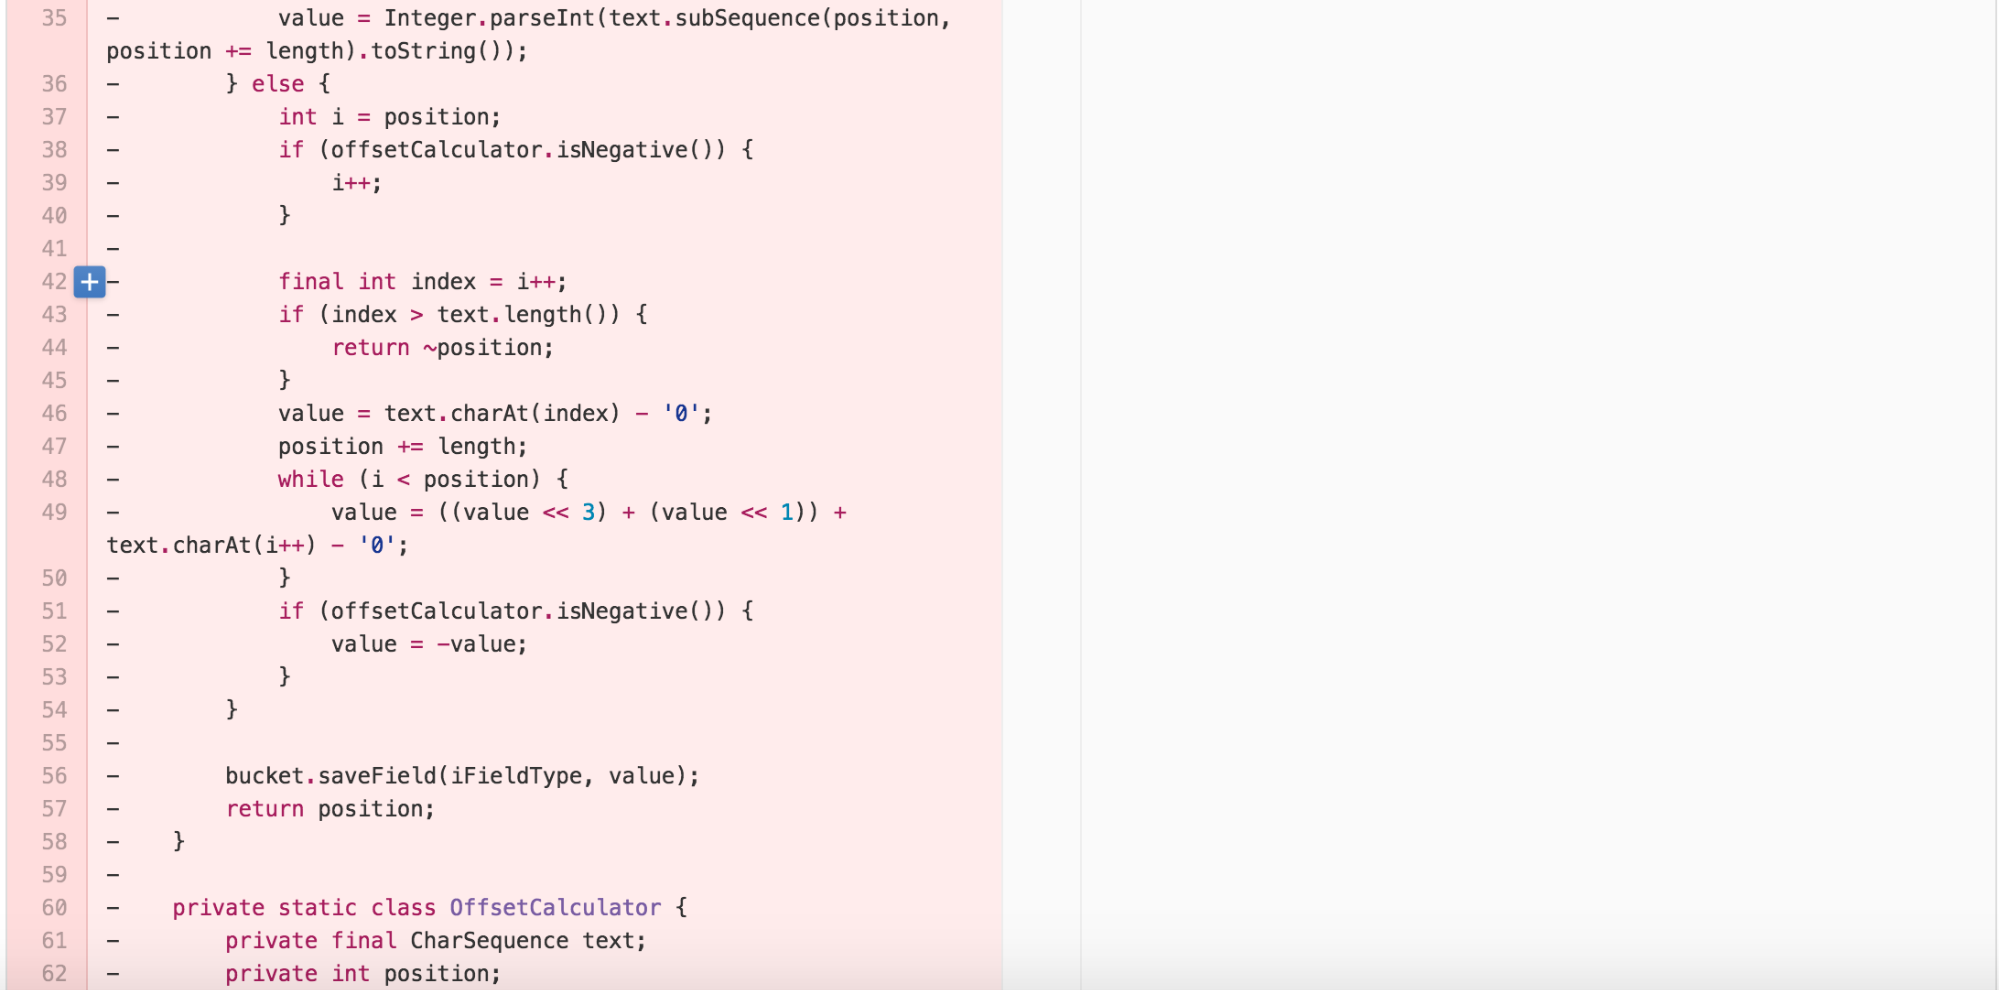
\includegraphics[width=\linewidth]{code24}
	\caption{insert caption}
\end{figure}
\begin{figure}[H]
	\centering
	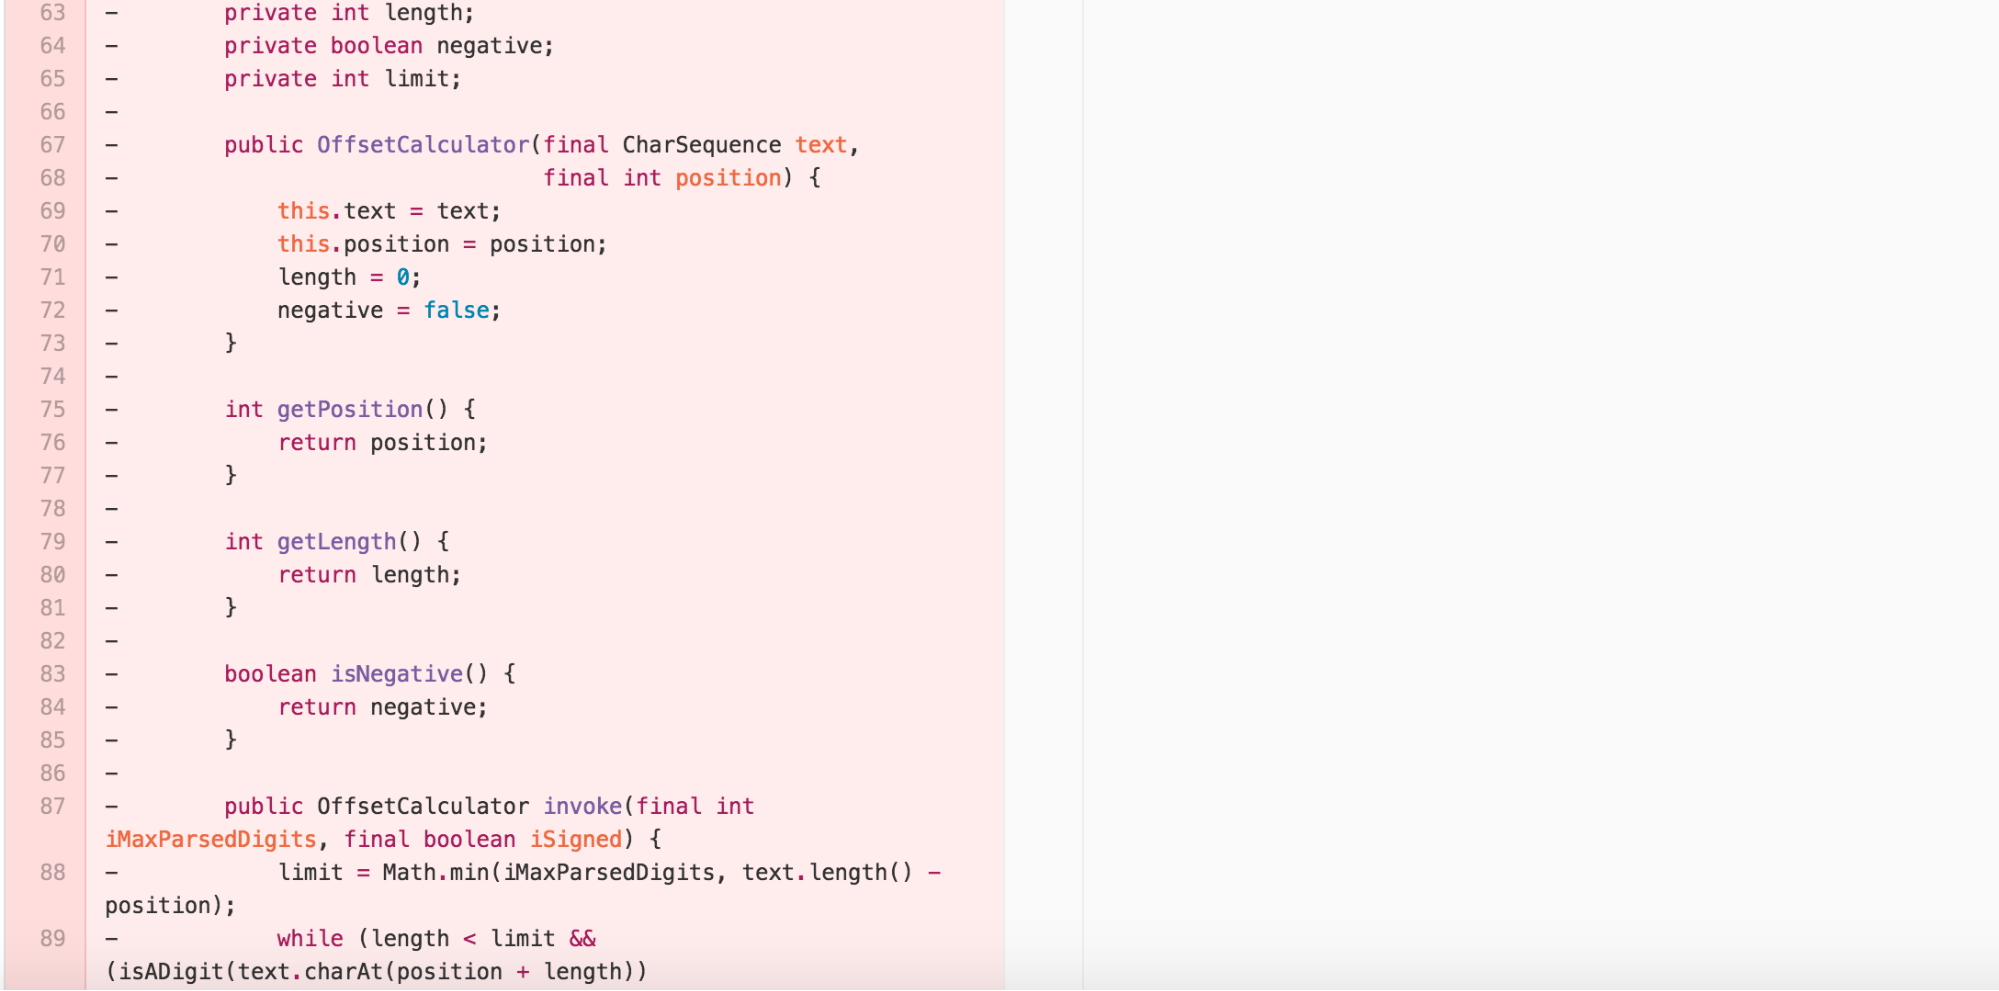
\includegraphics[width=\linewidth]{code25}
	\caption{insert caption}
\end{figure}
\begin{figure}[H]
	\centering
	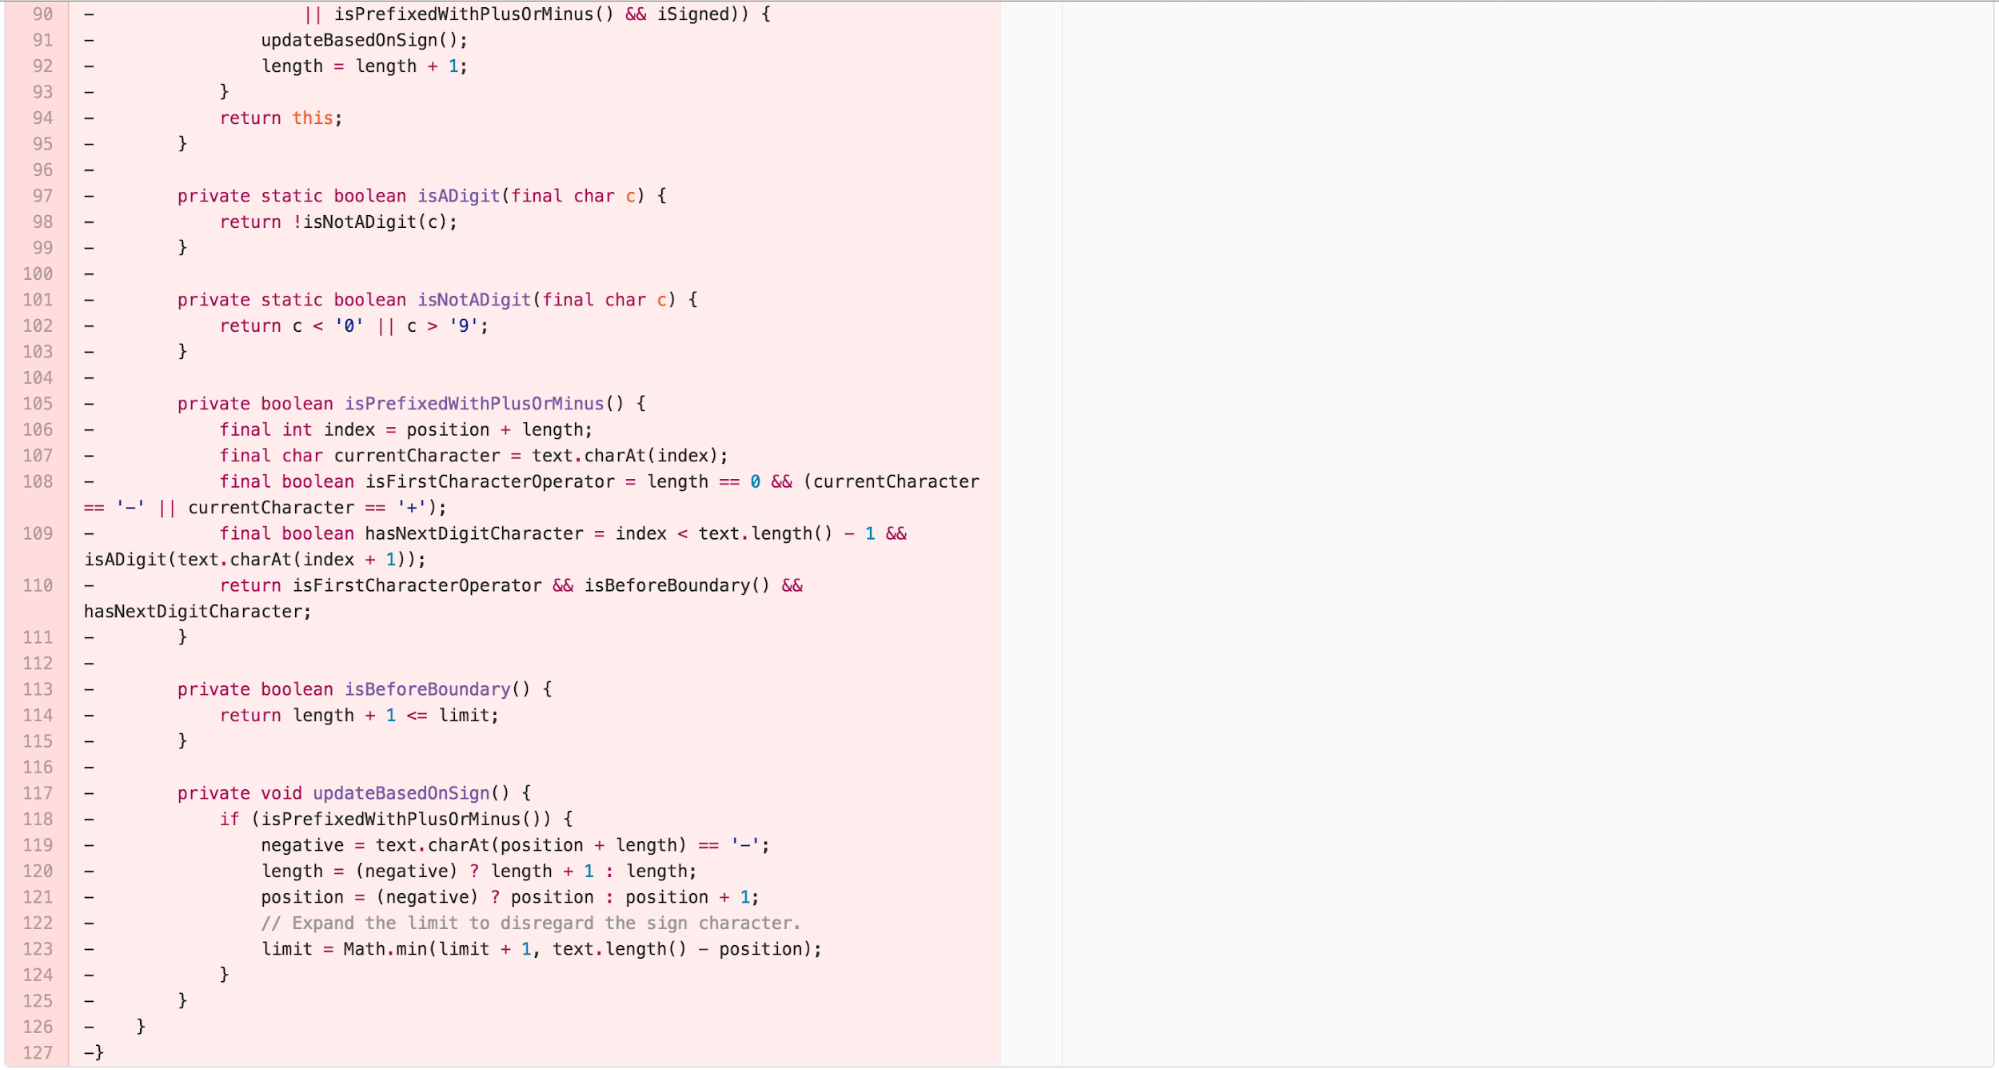
\includegraphics[width=\linewidth]{code26}
	\caption{insert caption}
\end{figure}
\begin{figure}[H]
	\centering
	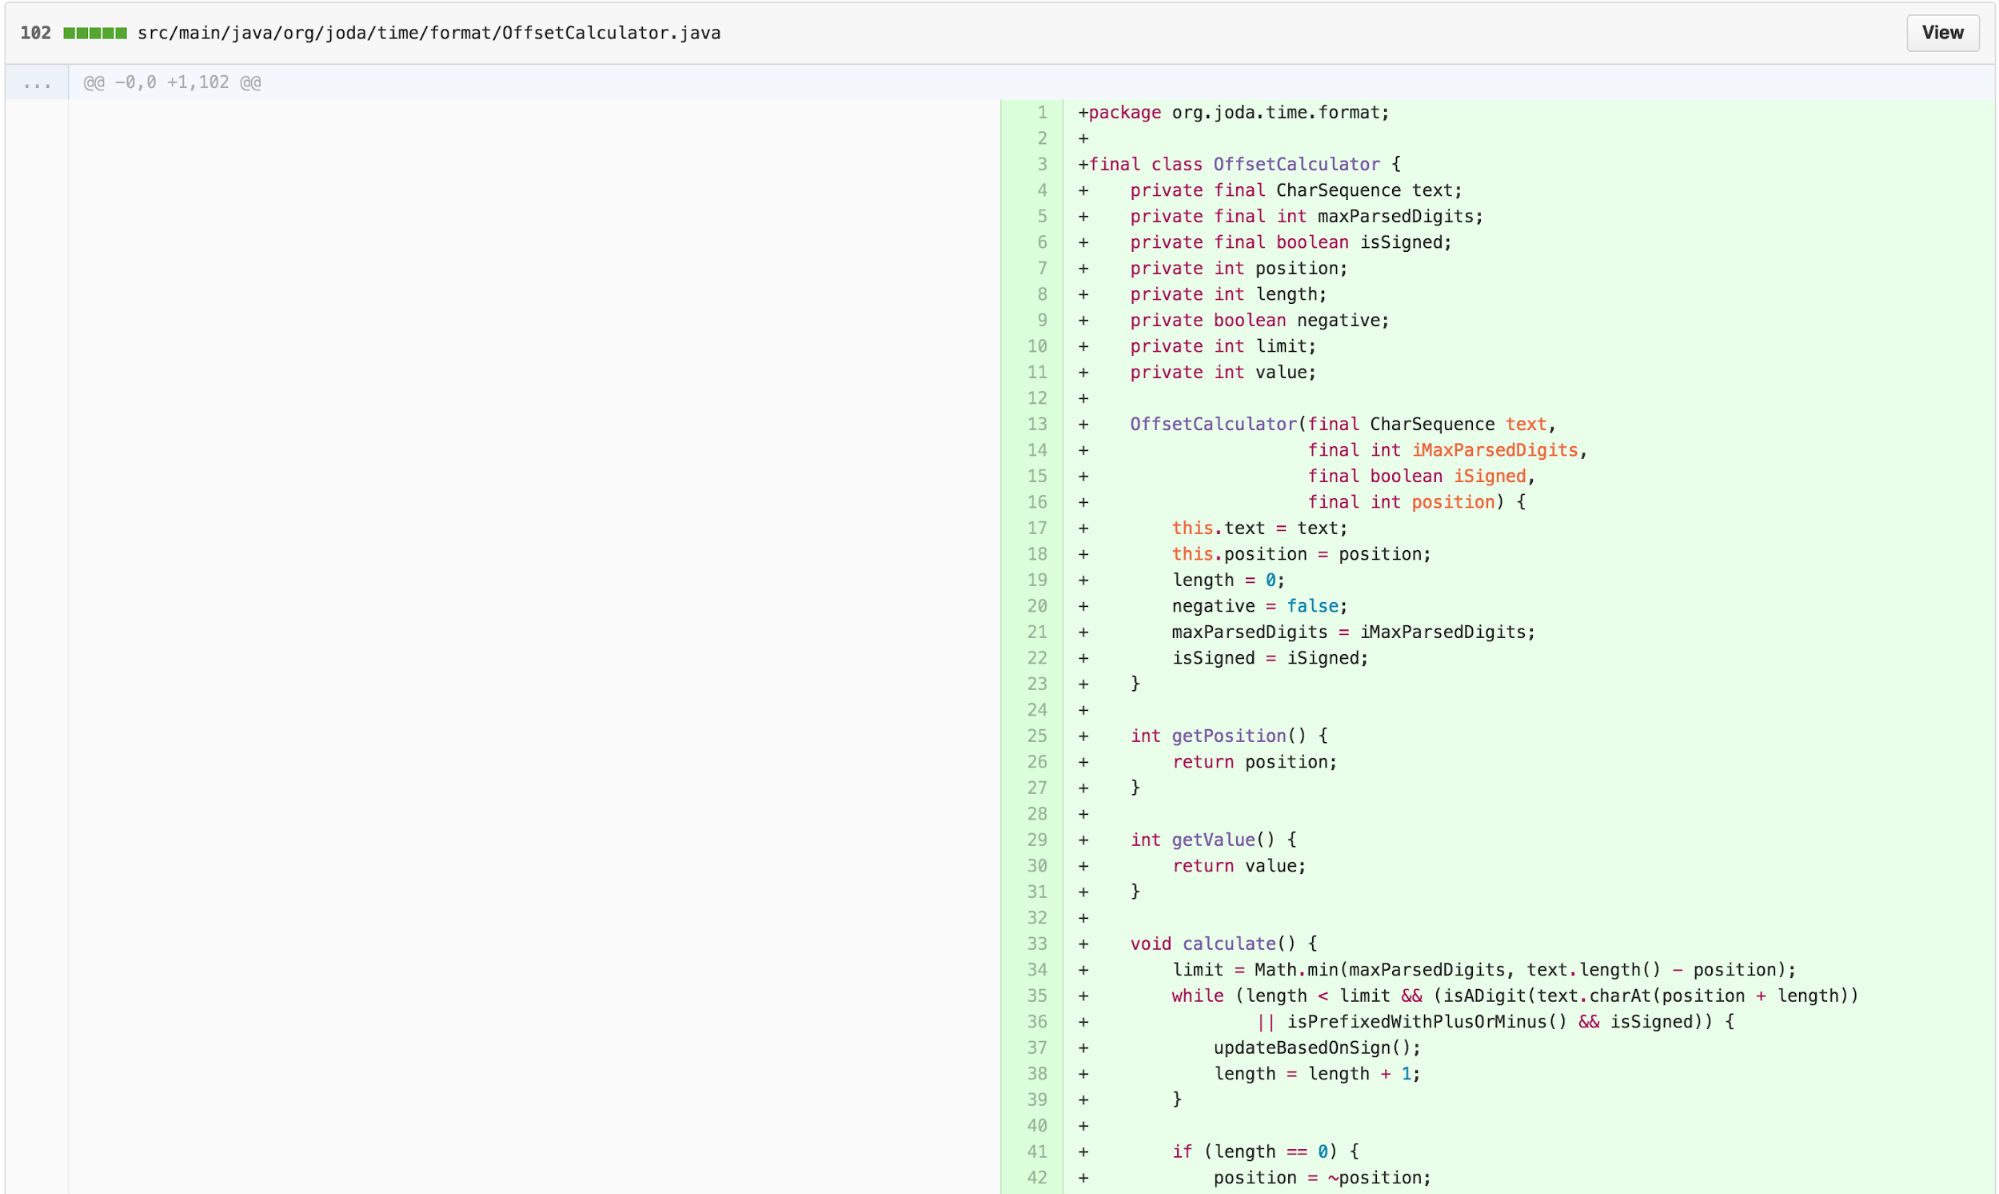
\includegraphics[width=\linewidth]{code27}
	\caption{insert caption}
\end{figure}
\begin{figure}[H]
	\centering
	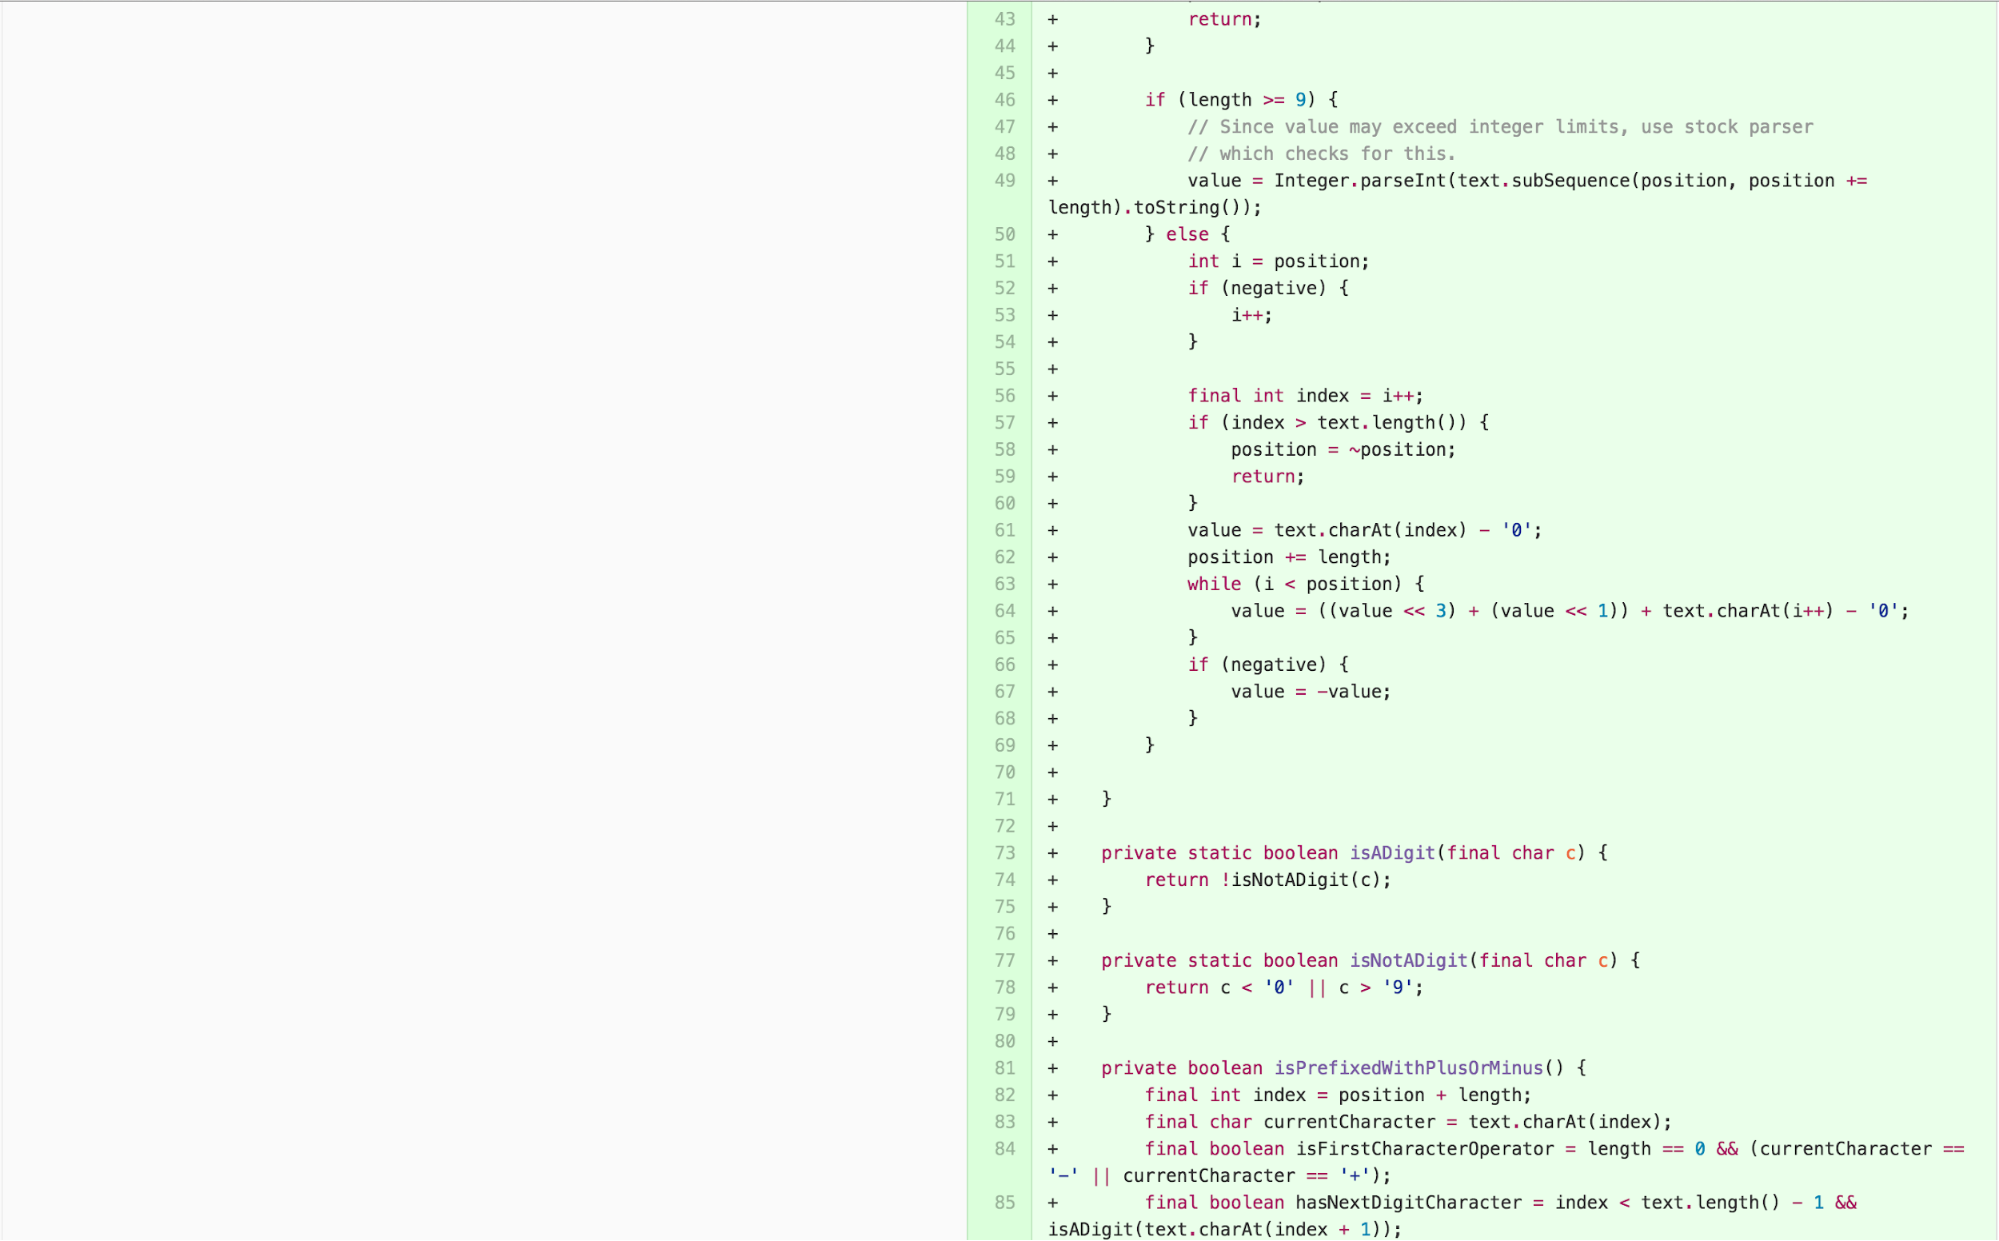
\includegraphics[width=\linewidth]{code28}
	\caption{insert caption}
\end{figure}
\begin{figure}[H]
	\centering
	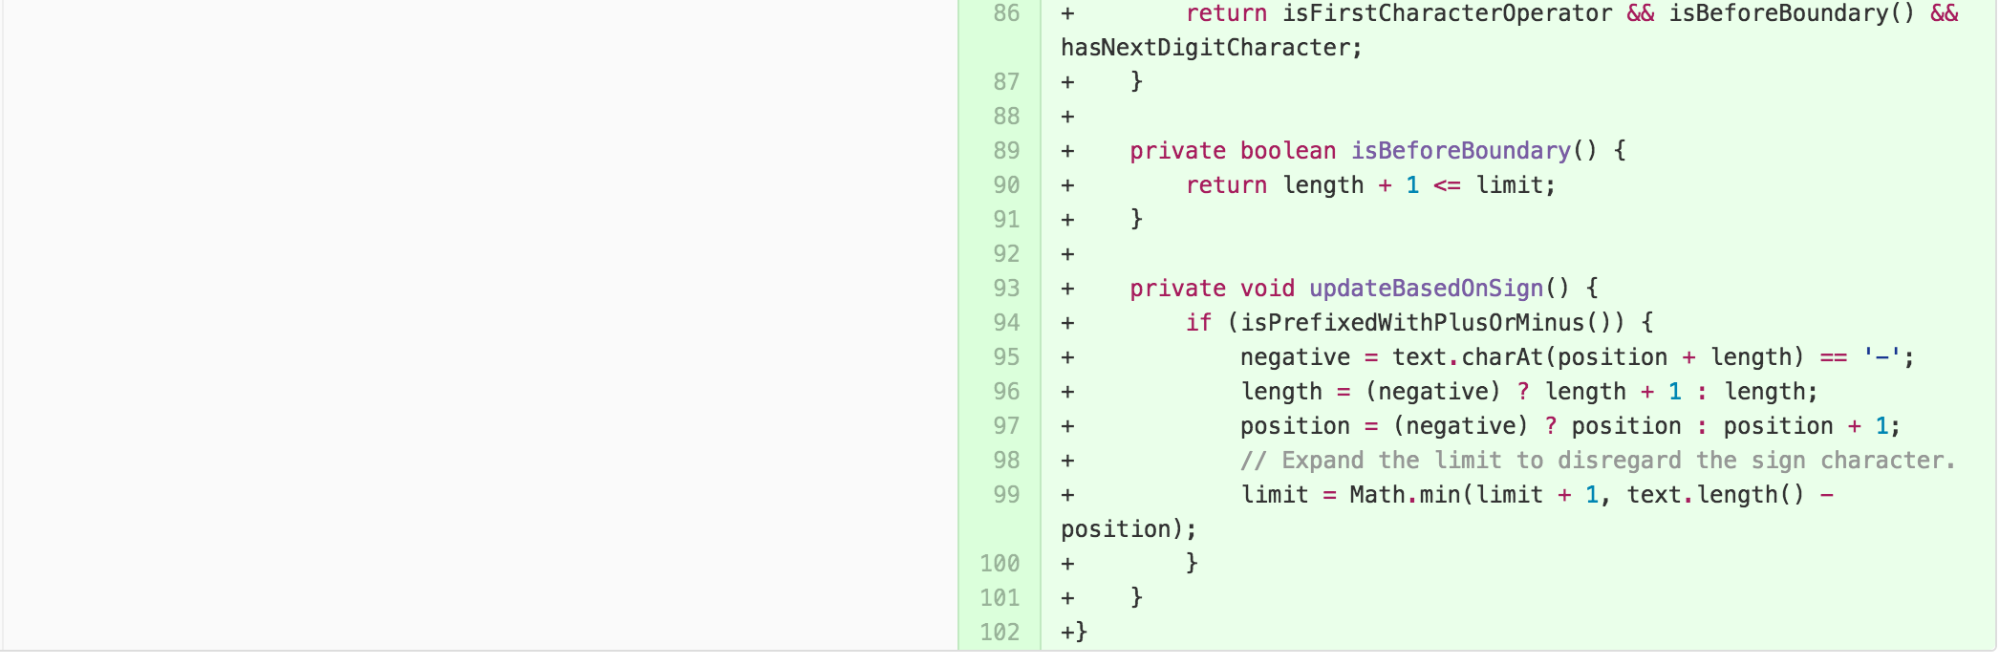
\includegraphics[width=\linewidth]{code29}
	\caption{insert caption}
\end{figure}

We can simplify the body of calculate further by applying EXTRACT METHOD, INTRODUCE EXPLAINING VARIABLE, and applying One Return Per Function, an arguably easier-to-understand practice stemming from the principles of Structured Programming, to simplify control.

\begin{figure}[H]
	\centering
	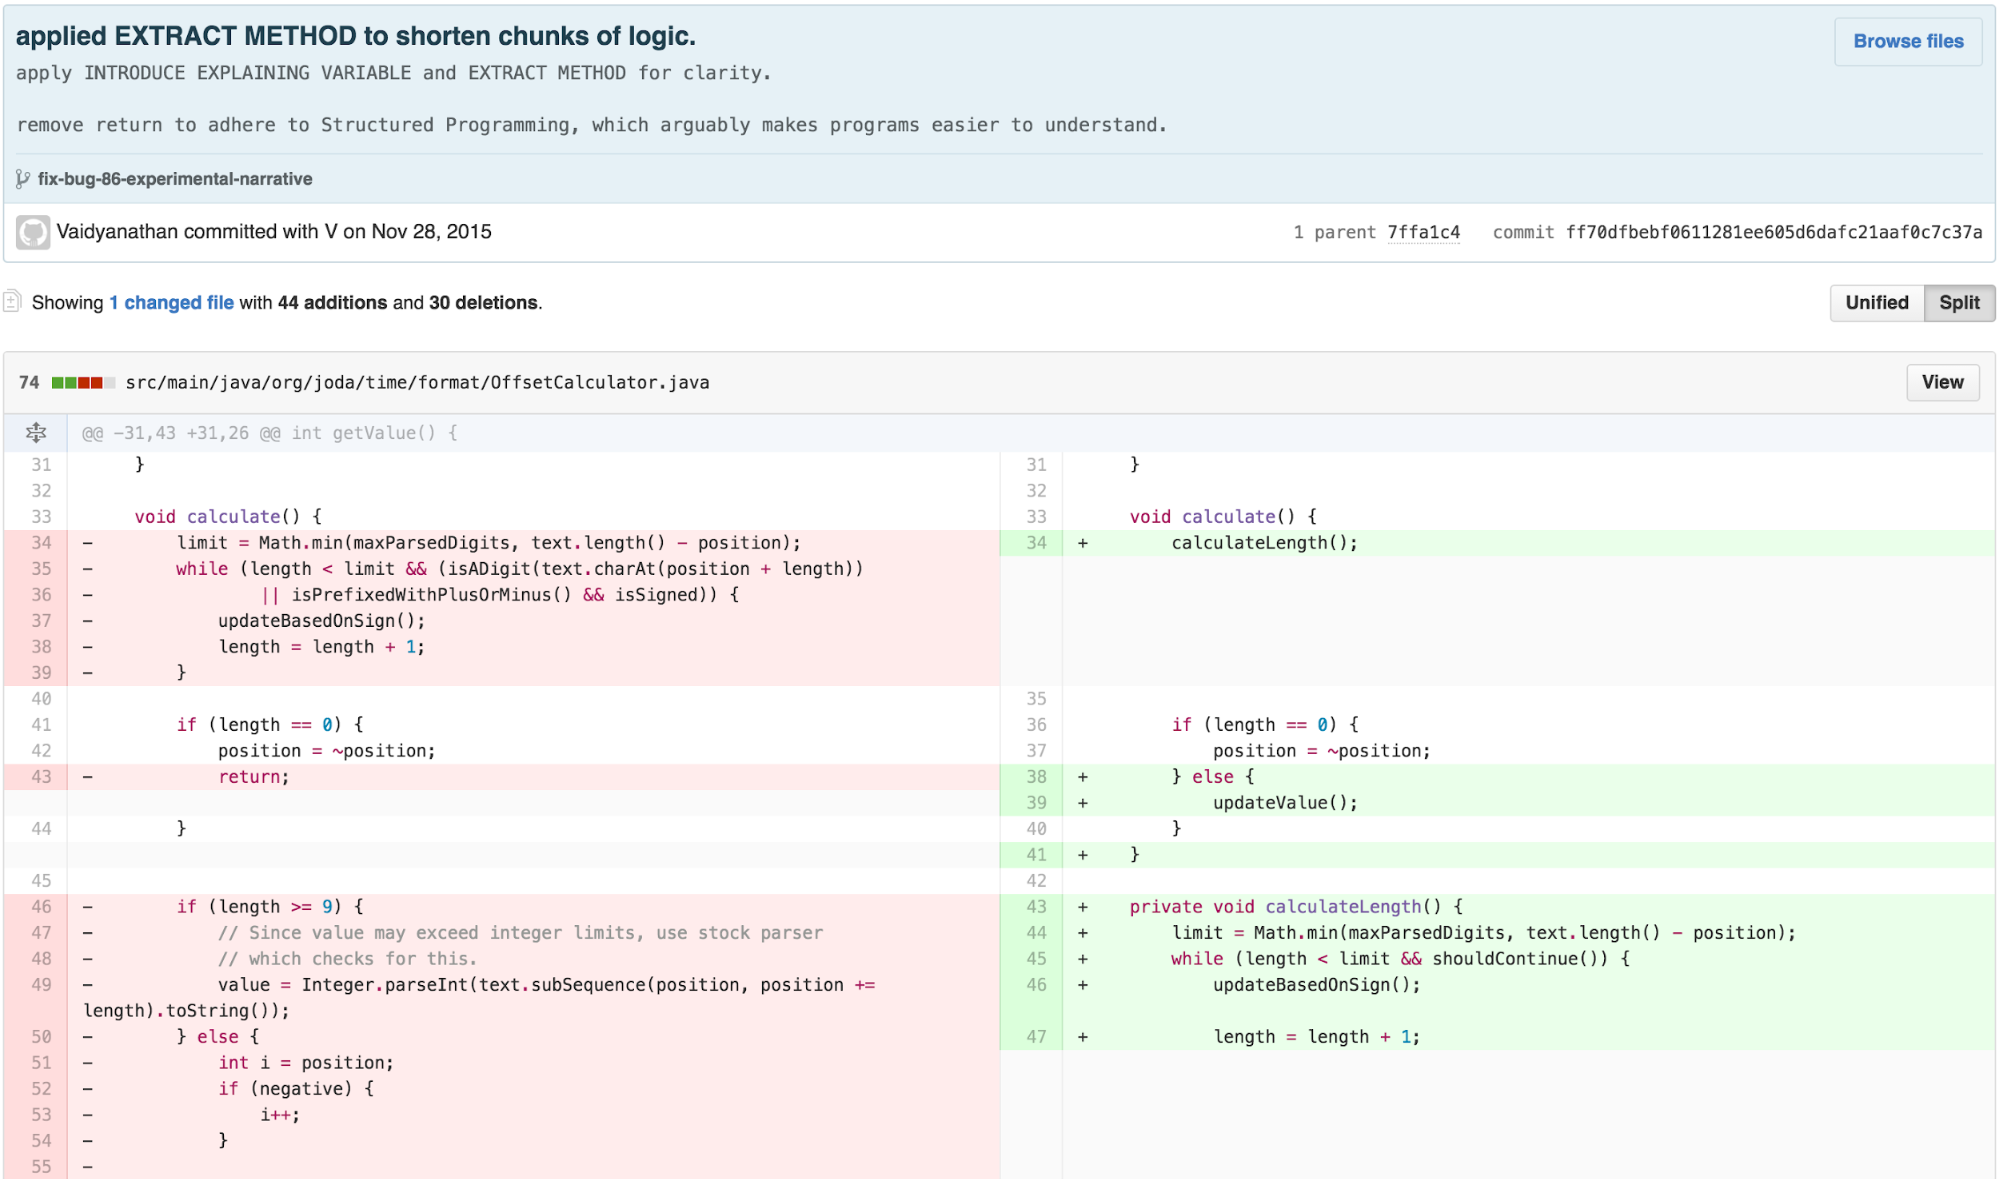
\includegraphics[width=\linewidth]{code30}
	\caption{insert caption}
\end{figure}
\begin{figure}[H]
	\centering
	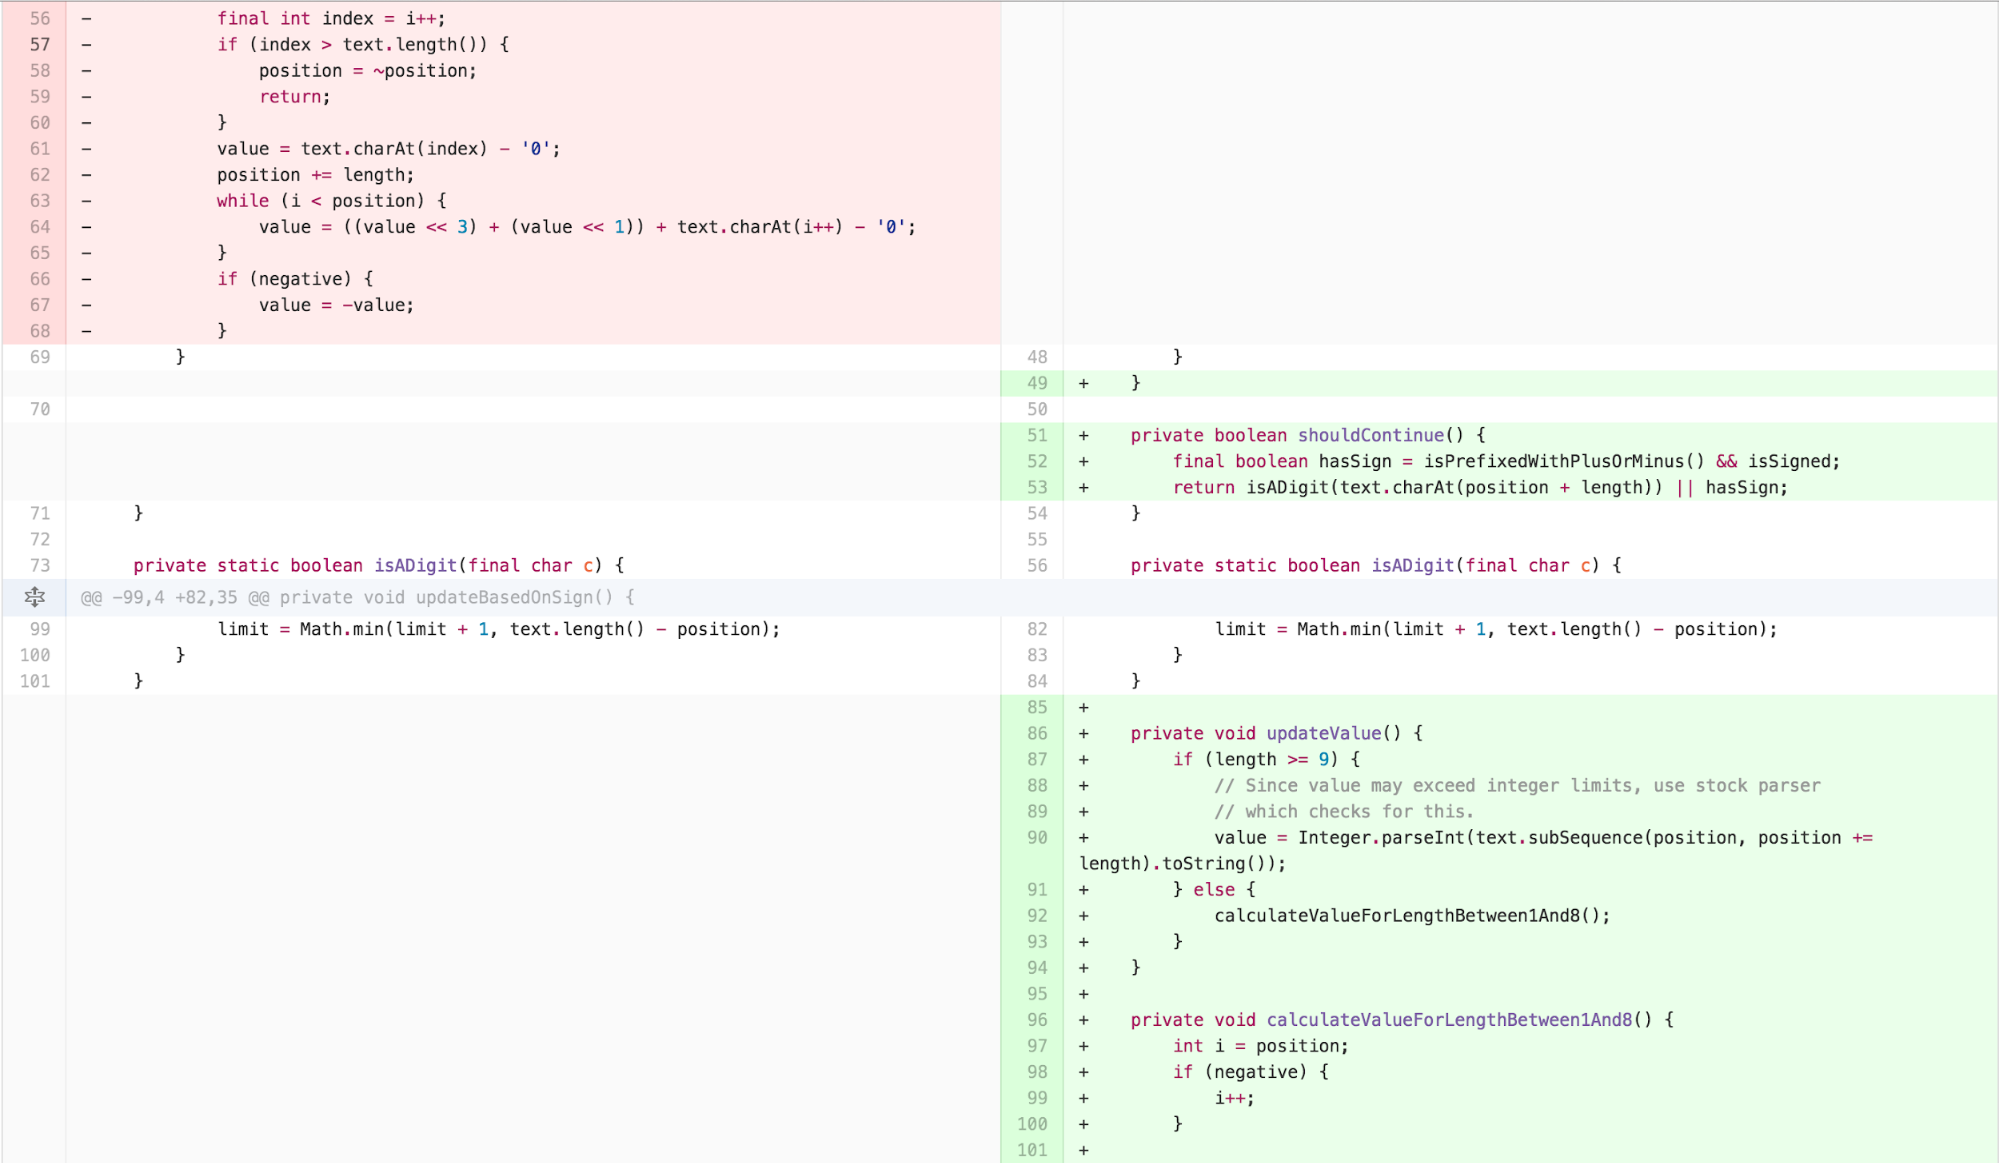
\includegraphics[width=\linewidth]{code31}
	\caption{insert caption}
\end{figure}
\begin{figure}[H]
	\centering
	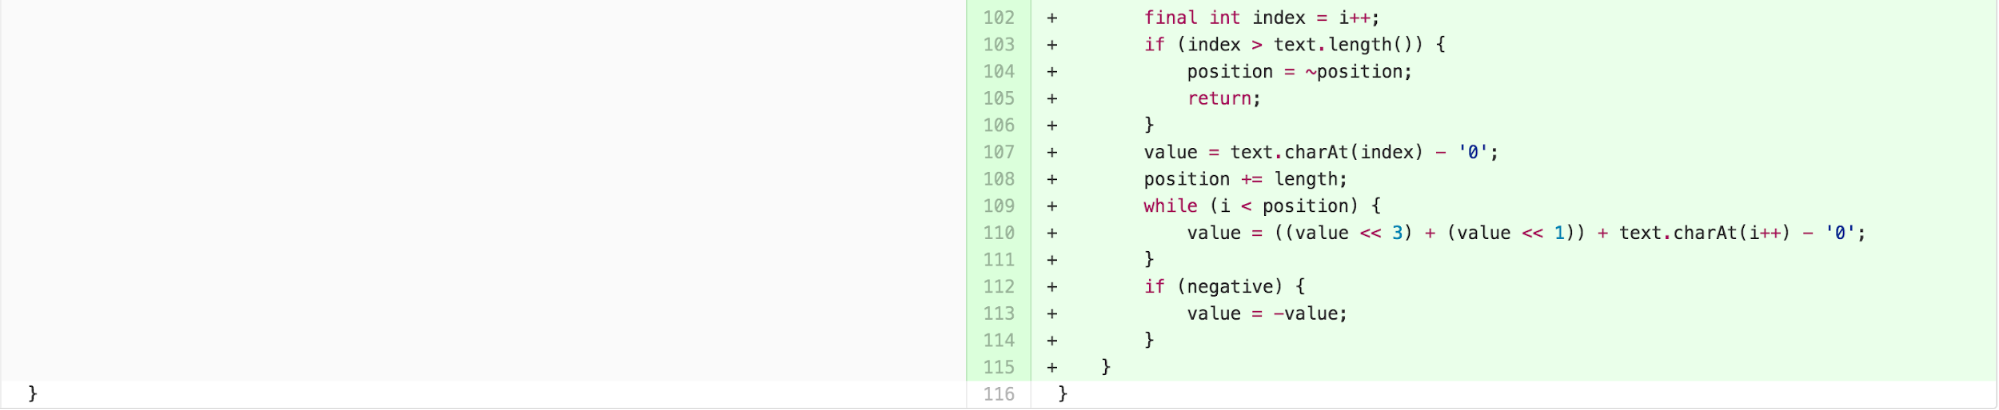
\includegraphics[width=\linewidth]{code32}
	\caption{insert caption}
\end{figure}

I then simplified the logic of \texttt{calculateValueForLengthBetween1And8} by applying EXTRACT METHOD and inverting the logic of the conditional, as Clean Code suggests negatives are harder to understand and the inversion allowed me to remove a return statement that broke control flow.

\begin{figure}[H]
	\centering
	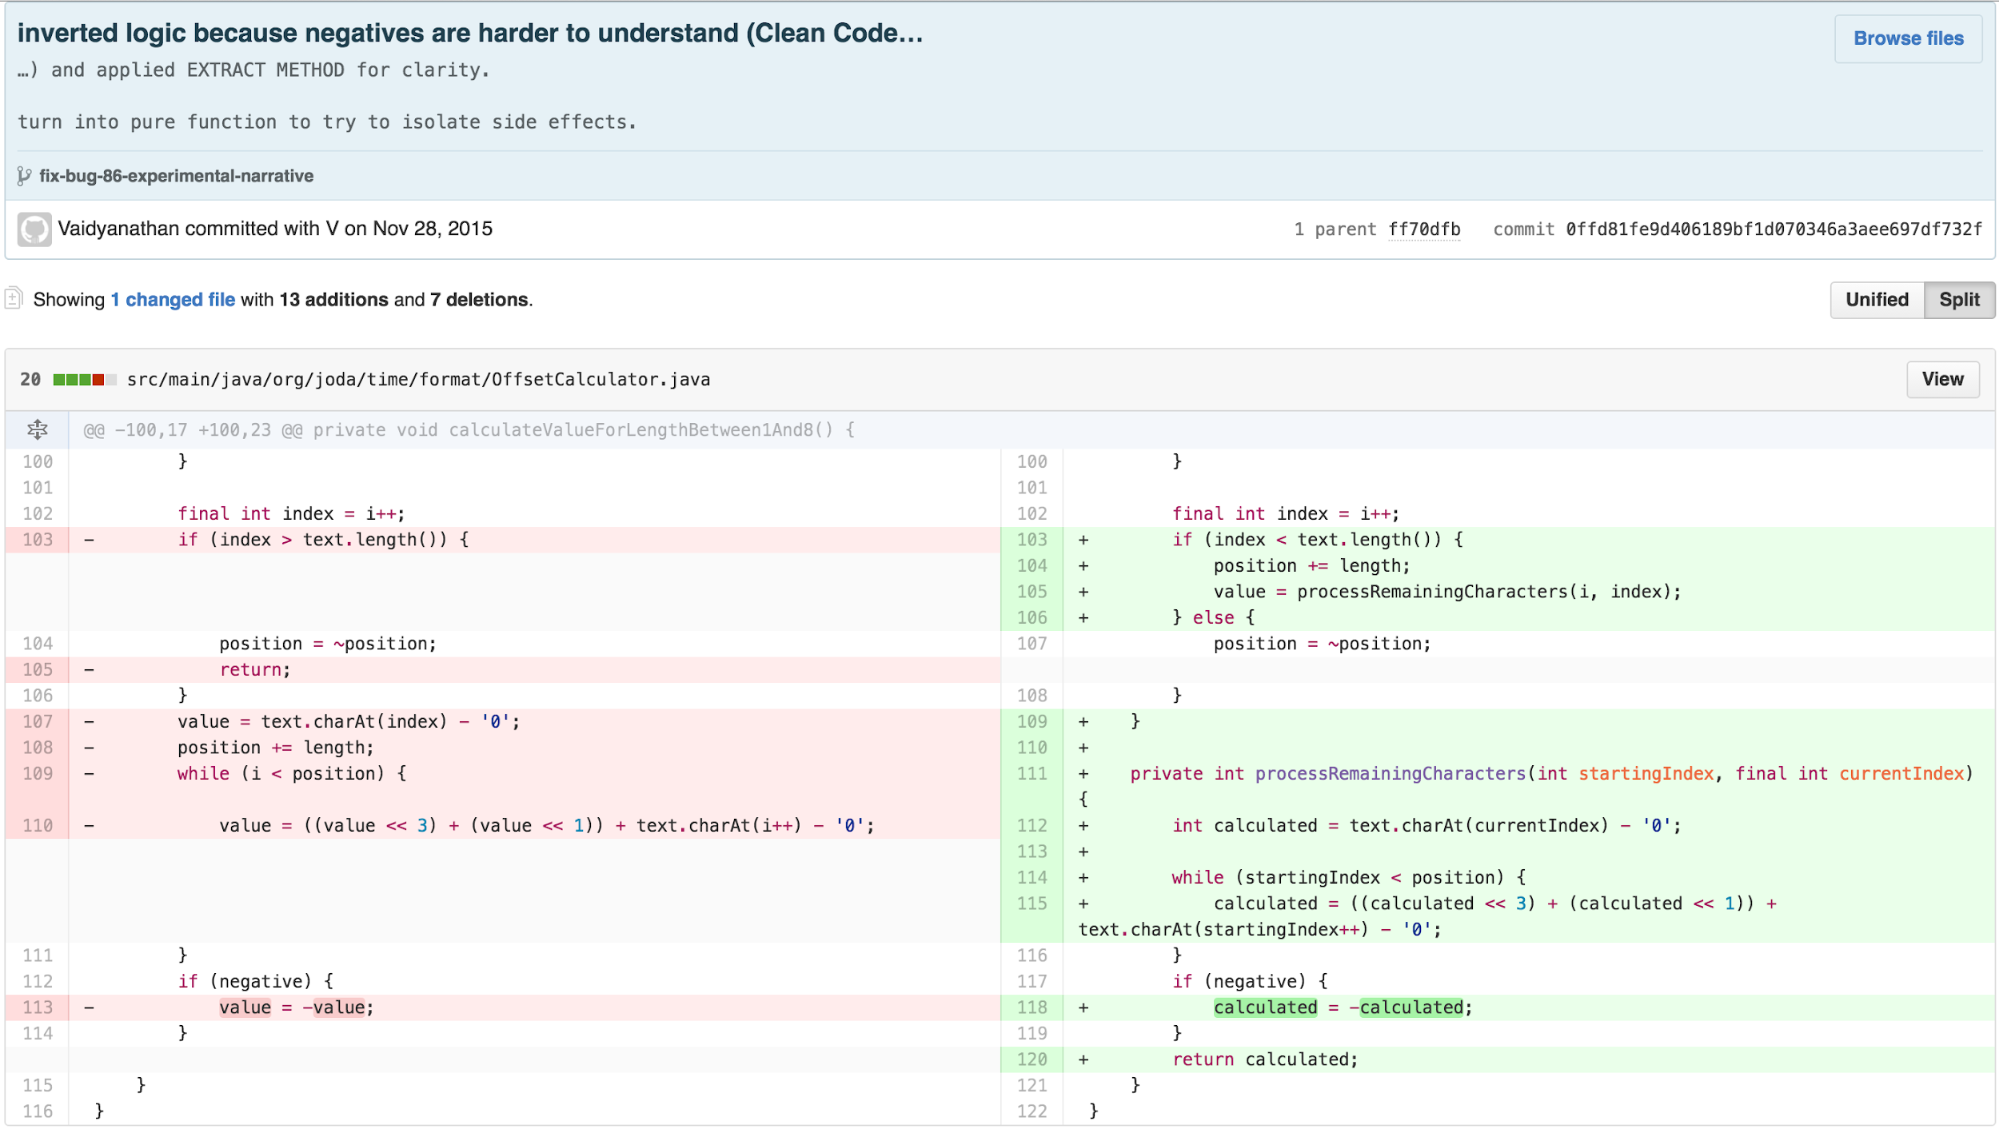
\includegraphics[width=\linewidth]{code33}
	\caption{insert caption}
\end{figure}

I then started seeking code to remove, as I detected that some of the methods were redundant from features already offered by the built-in Java libraries. I also applied further EXTRACT METHOD to describe the algorithm declaratively using names and separate the levels of abstraction according to the Newspaper Metaphor.

\begin{figure}[H]
	\centering
	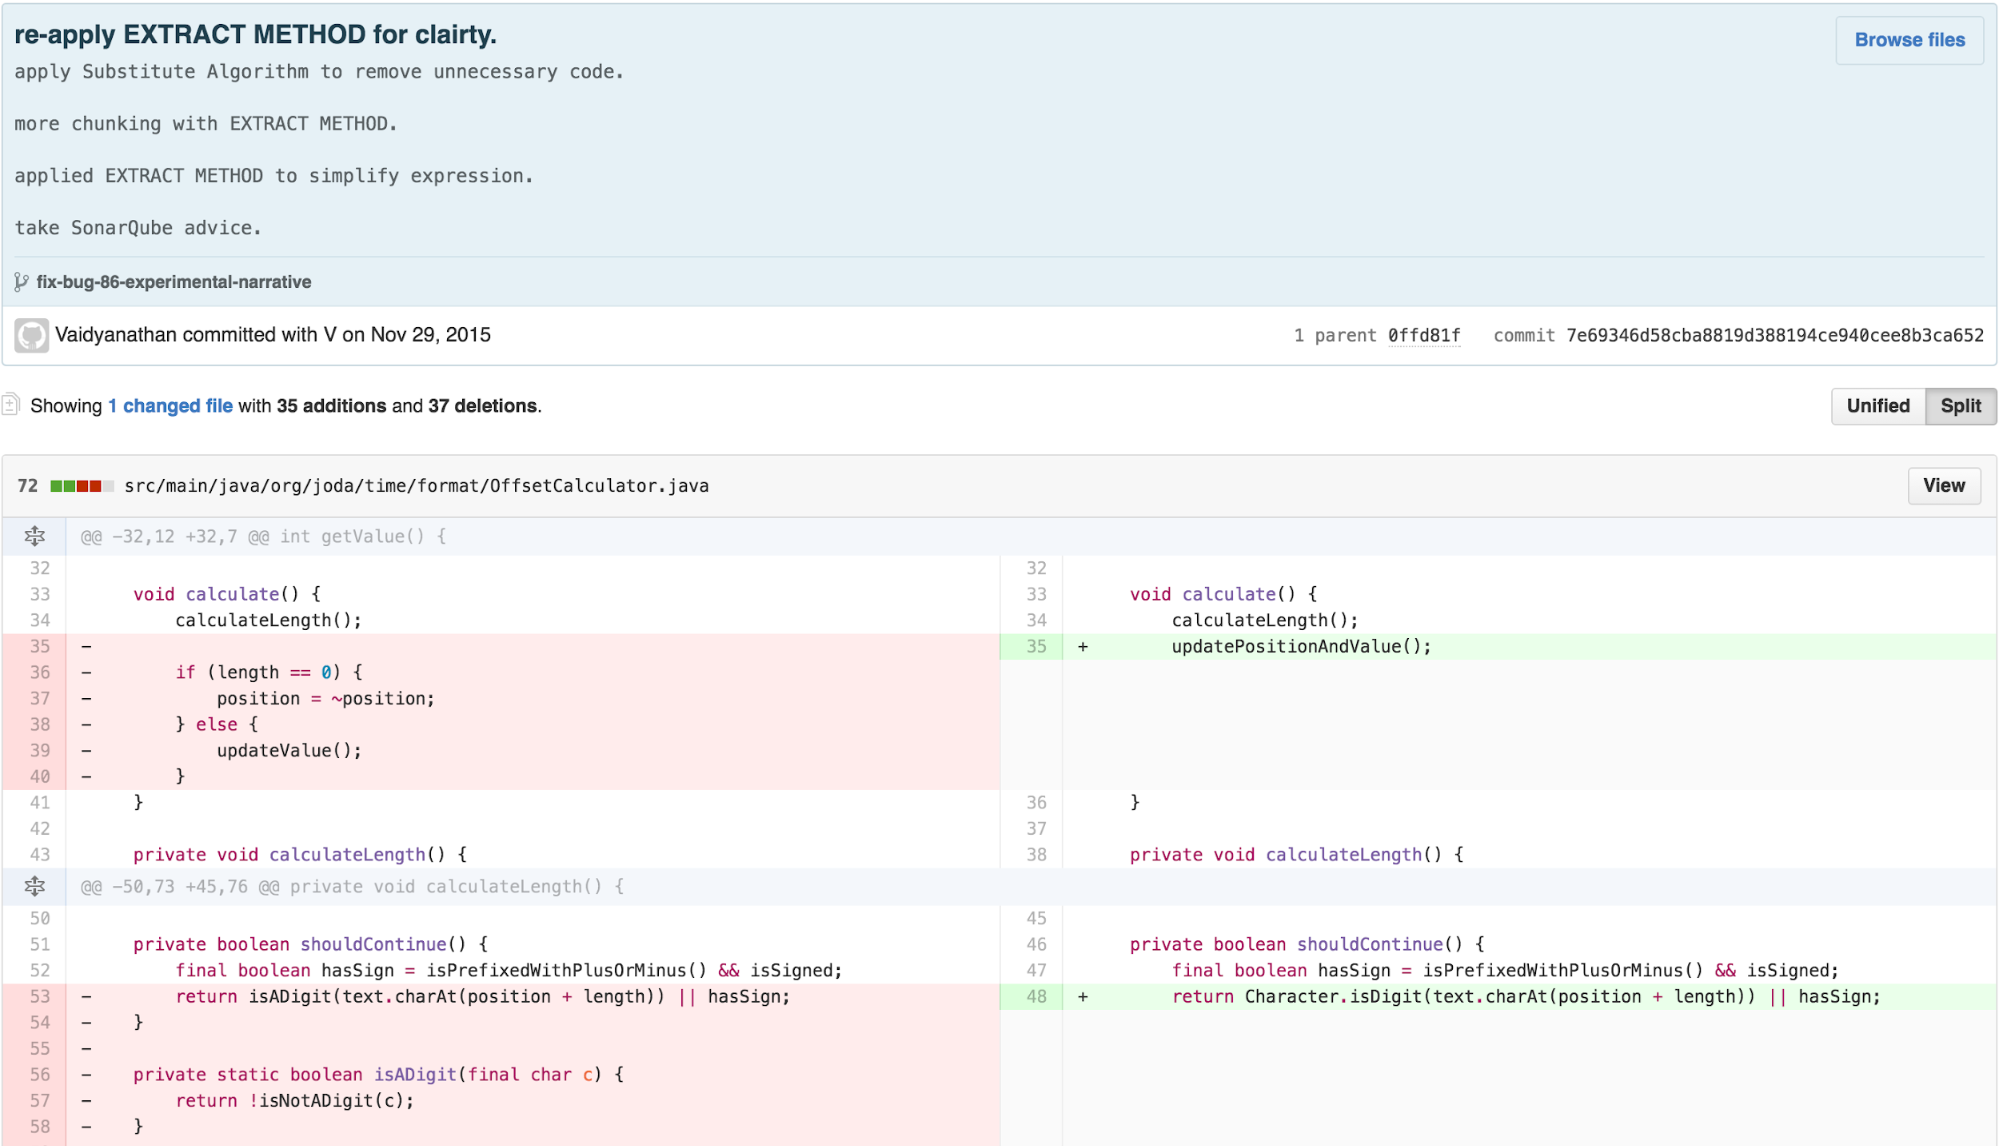
\includegraphics[width=\linewidth]{code34}
	\caption{insert caption}
\end{figure}
\begin{figure}[H]
	\centering
	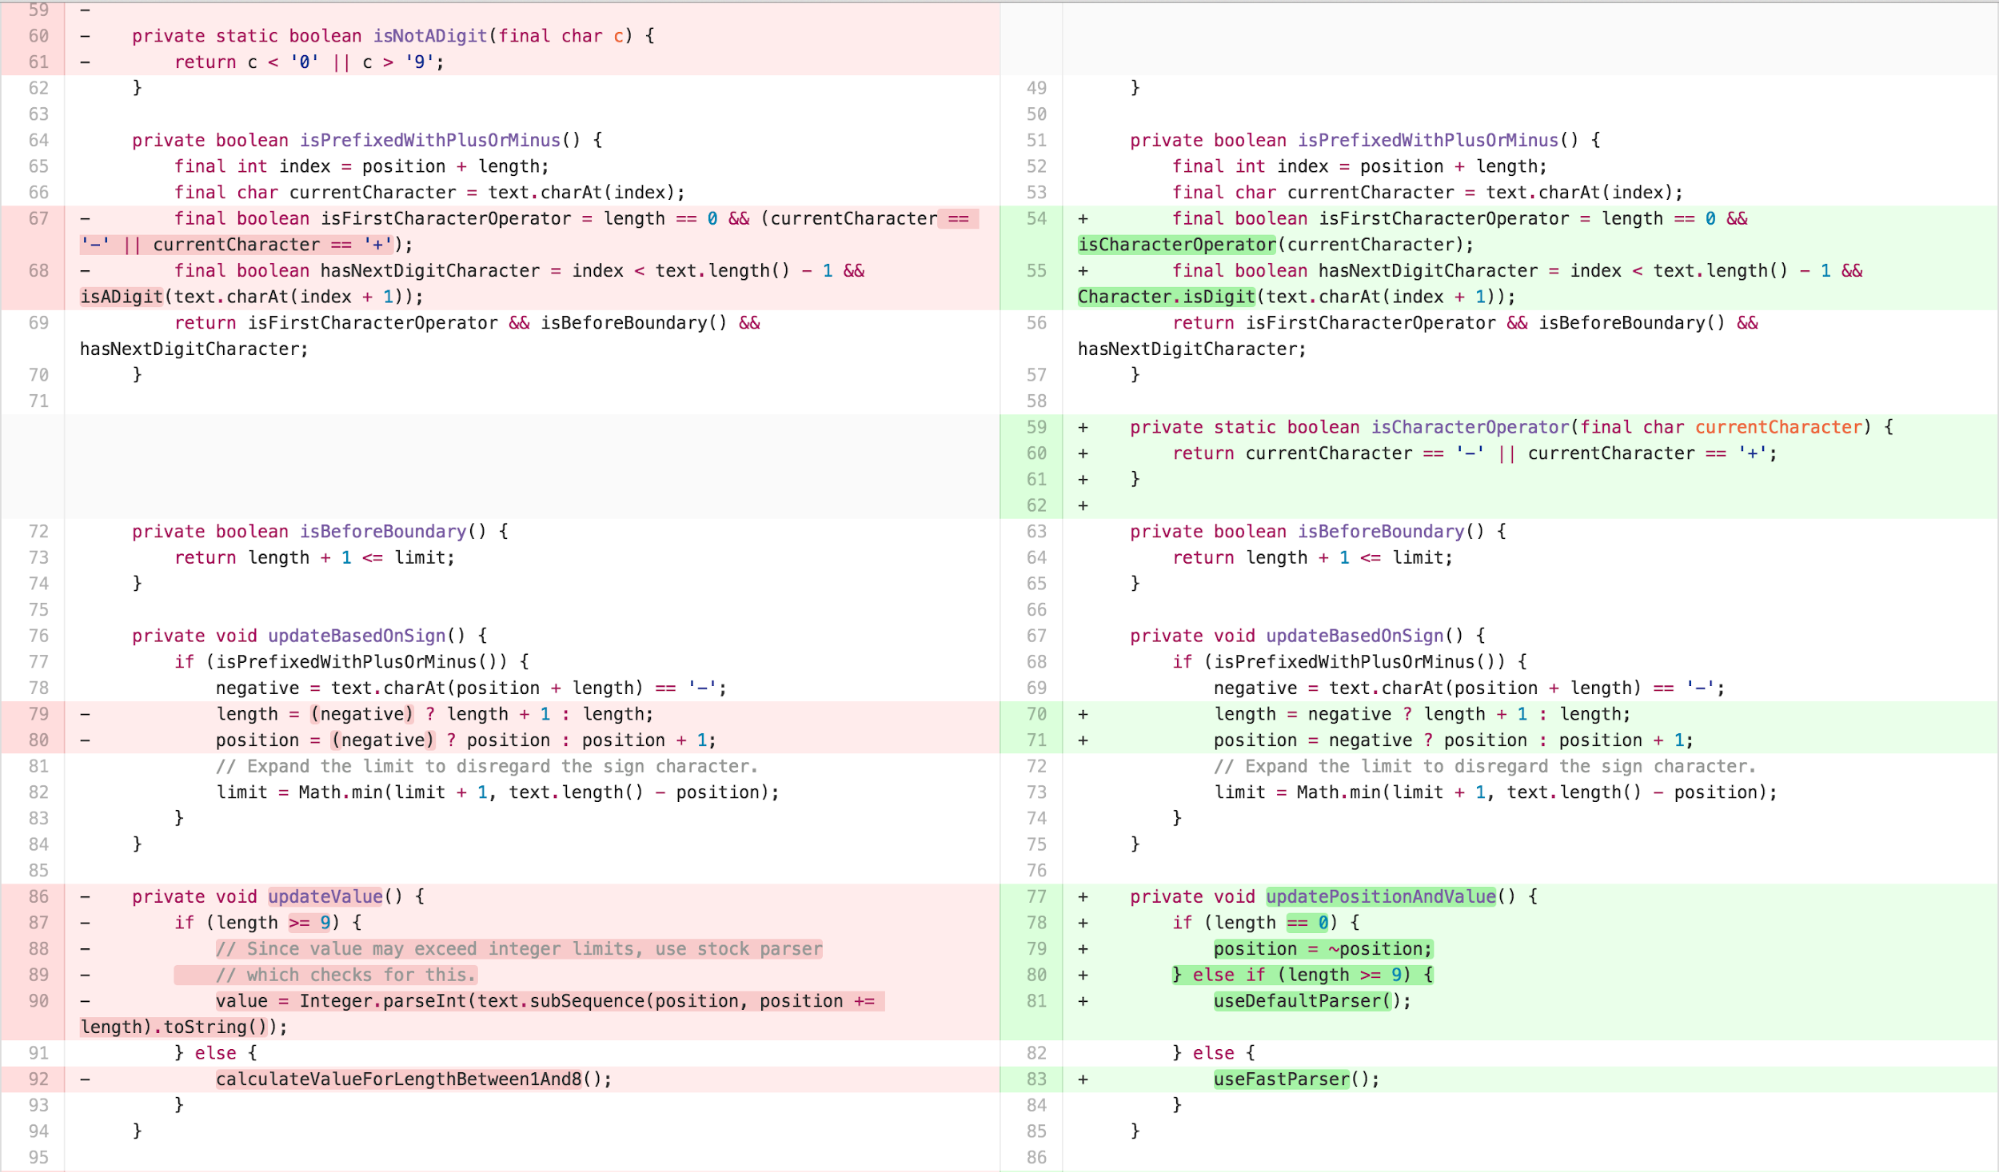
\includegraphics[width=\linewidth]{code35}
	\caption{insert caption}
\end{figure}
\begin{figure}[H]
	\centering
	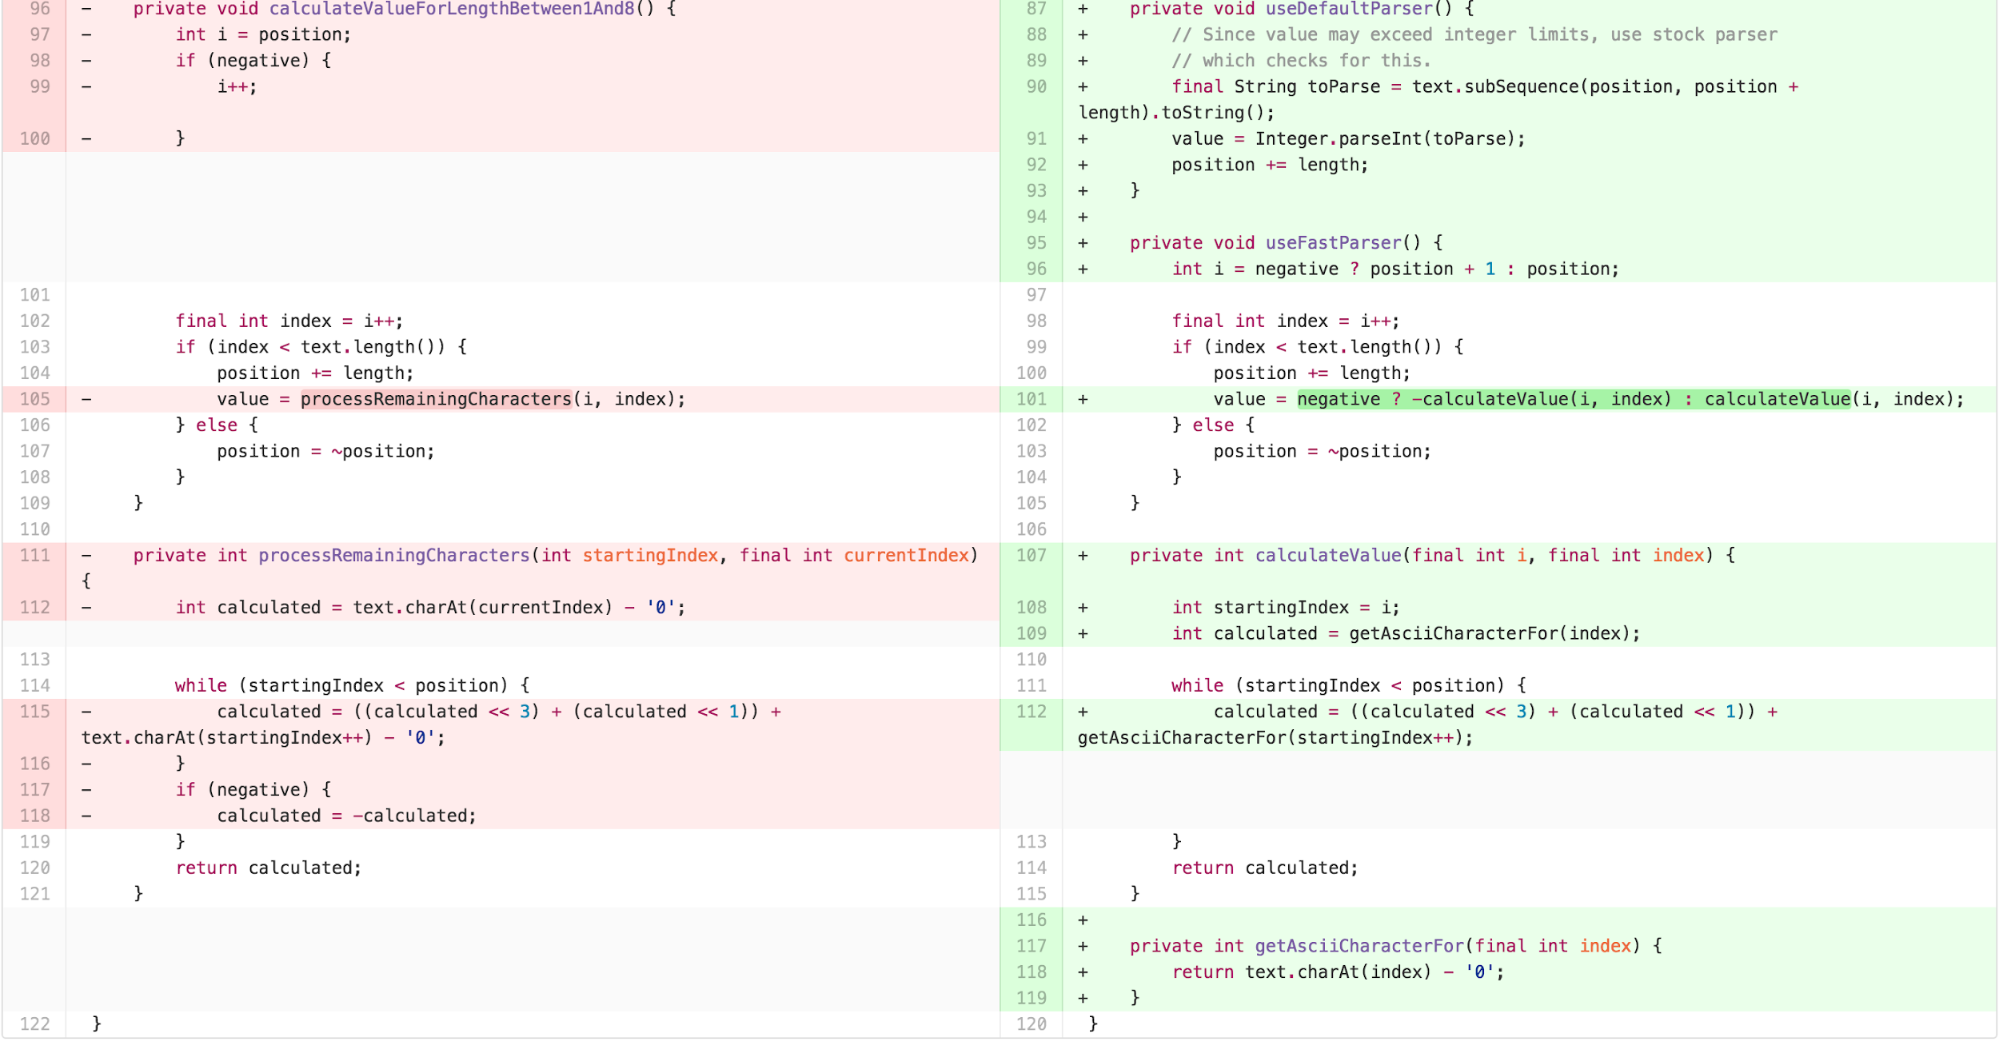
\includegraphics[width=\linewidth]{code36}
	\caption{insert caption}
\end{figure}

At this point, from a pure “code metrics” perspective, \texttt{OffsetCalculator} was significantly simpler. Each method was no more than 9 lines long, the class had 3 getter methods, 3 “utility” style 1-line descriptive methods, and 8 “logical” methods. Being pretty experienced with the code at this point, it was fairly easy for me to see where to “apply the fix” to resolve the bug in this reduced scope. 

\subsection{Checking my biases: adapting to peer feedback}
I was pretty confident the new code would be significantly easier to understand. In order to validate this hypothesis, I sought feedback from some expert and novice software engineers. In these dry-run, non-formal talk throughs, I discovered something surprising. Although the \texttt{OffsetCalculator} was chunked well for comprehensibility, its overall role within the parsing process was difficult to understand. The obviously tricky \texttt{useFastParser()} that used bit shifting was cognitively dense, but even the calculation of length and position that immediately preceded it were difficult to grok in terms of the intent of the calculation. Initial passes at debugging showed that the architecture itself, from the relationship of the \texttt{DateTimeFormatter} to the \texttt{DateTimeFormatterBuilder} to the \texttt{NumberFormatter} to the \texttt{OffsetCalculator}, was complex. I realized I need to spend more time with the \texttt{DateTimeFormatter} to make it easier to bypass its functionality and get to the \texttt{OffsetCalculator} quicker.

\subsection{Architectural adaptation: Simplifying DateTimeFormatter}

I started with applying EXTRACT METHOD on spots of obvious duplication the calculation of Chronology, into a method called \texttt{getChronology}. I then saw repeated duplication with only detail variation in \texttt{parseDateTime}, \texttt{parseLocalDateTime}, and \texttt{parseMutableDateTime}, so I extracted what was different in those methods out. In order to create a seam for myself to be able to move the body of those methods into an independently simplified piece without changing the externally facing interface, I extracted the body of the public methods into separate internal private methods.

\begin{figure}[H]
	\centering
	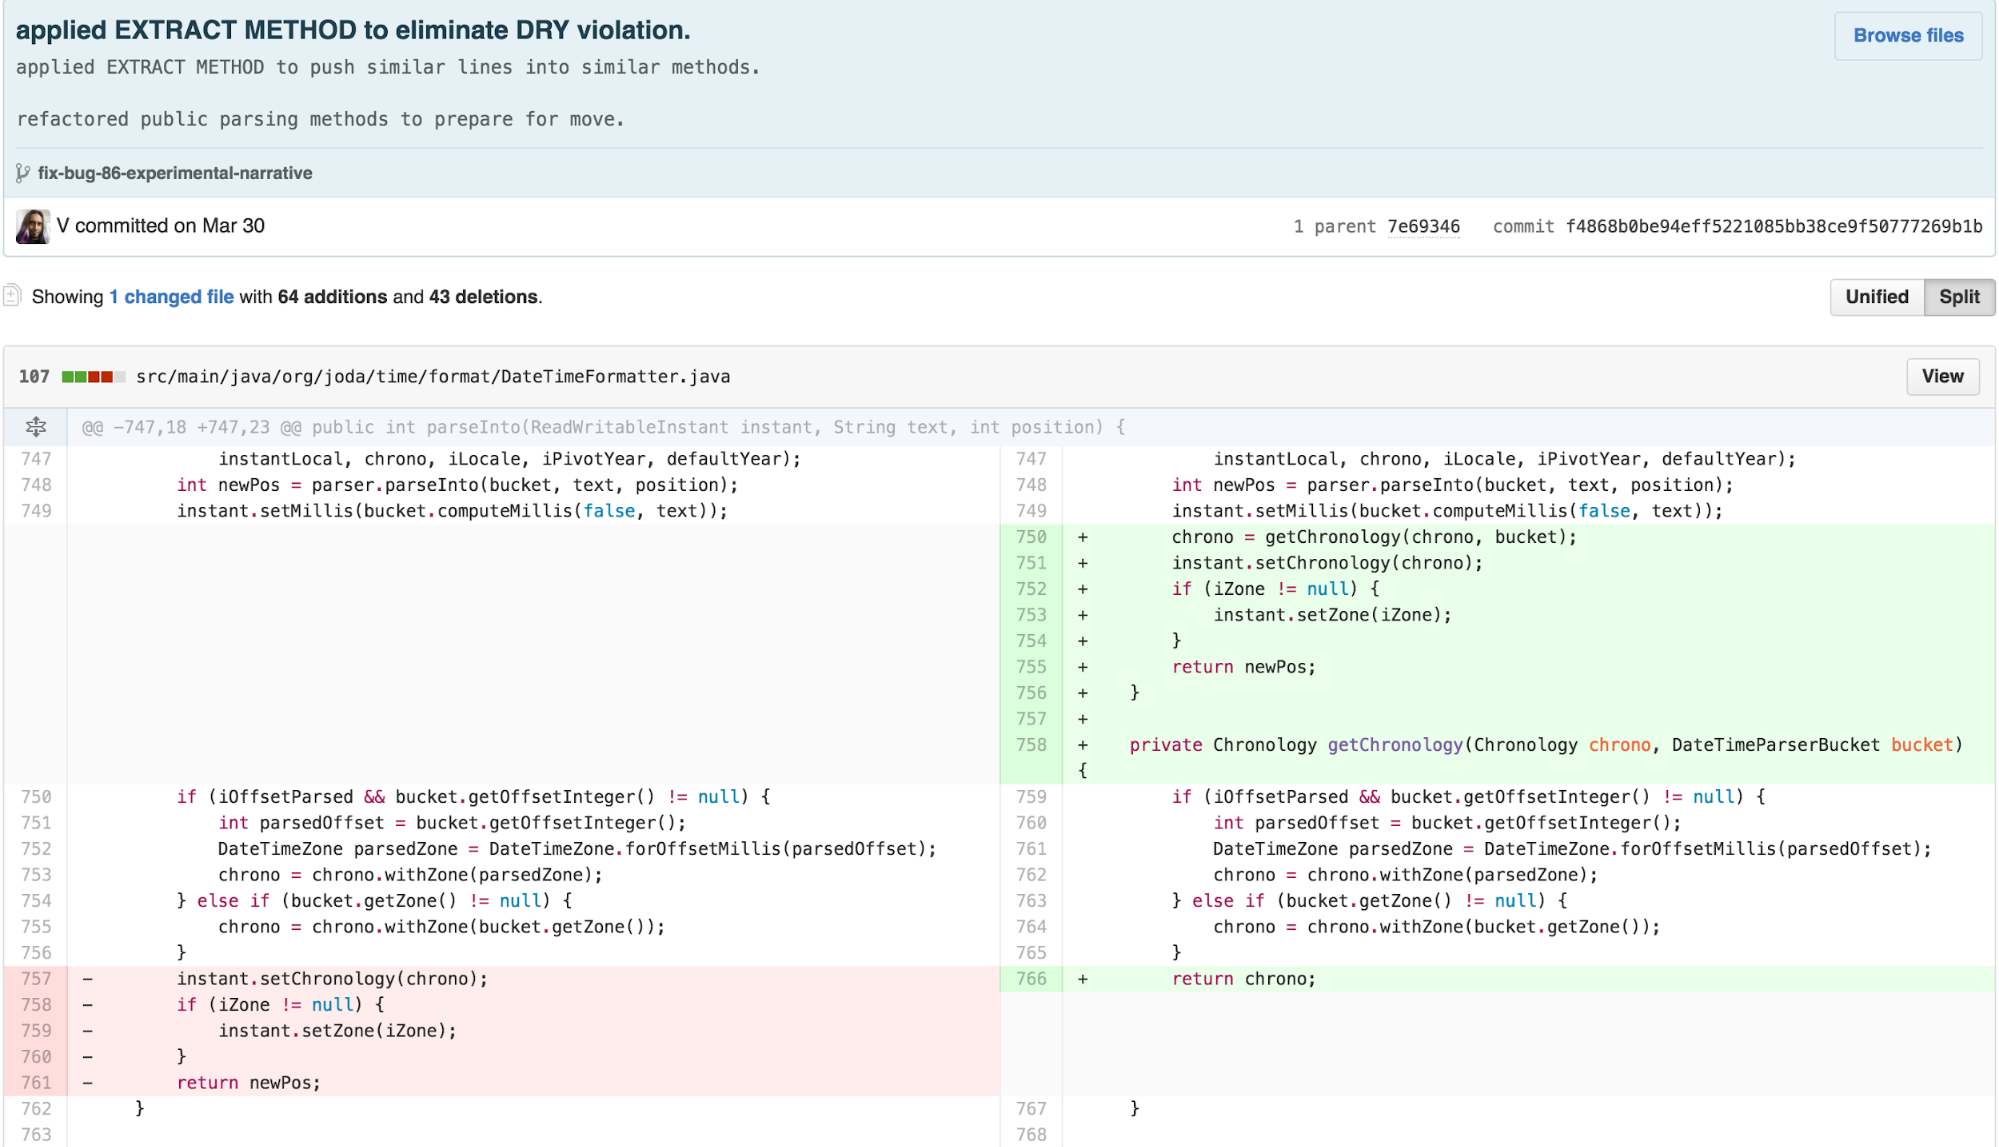
\includegraphics[width=\linewidth]{code37}
	\caption{insert caption}
\end{figure}
\begin{figure}[H]
	\centering
	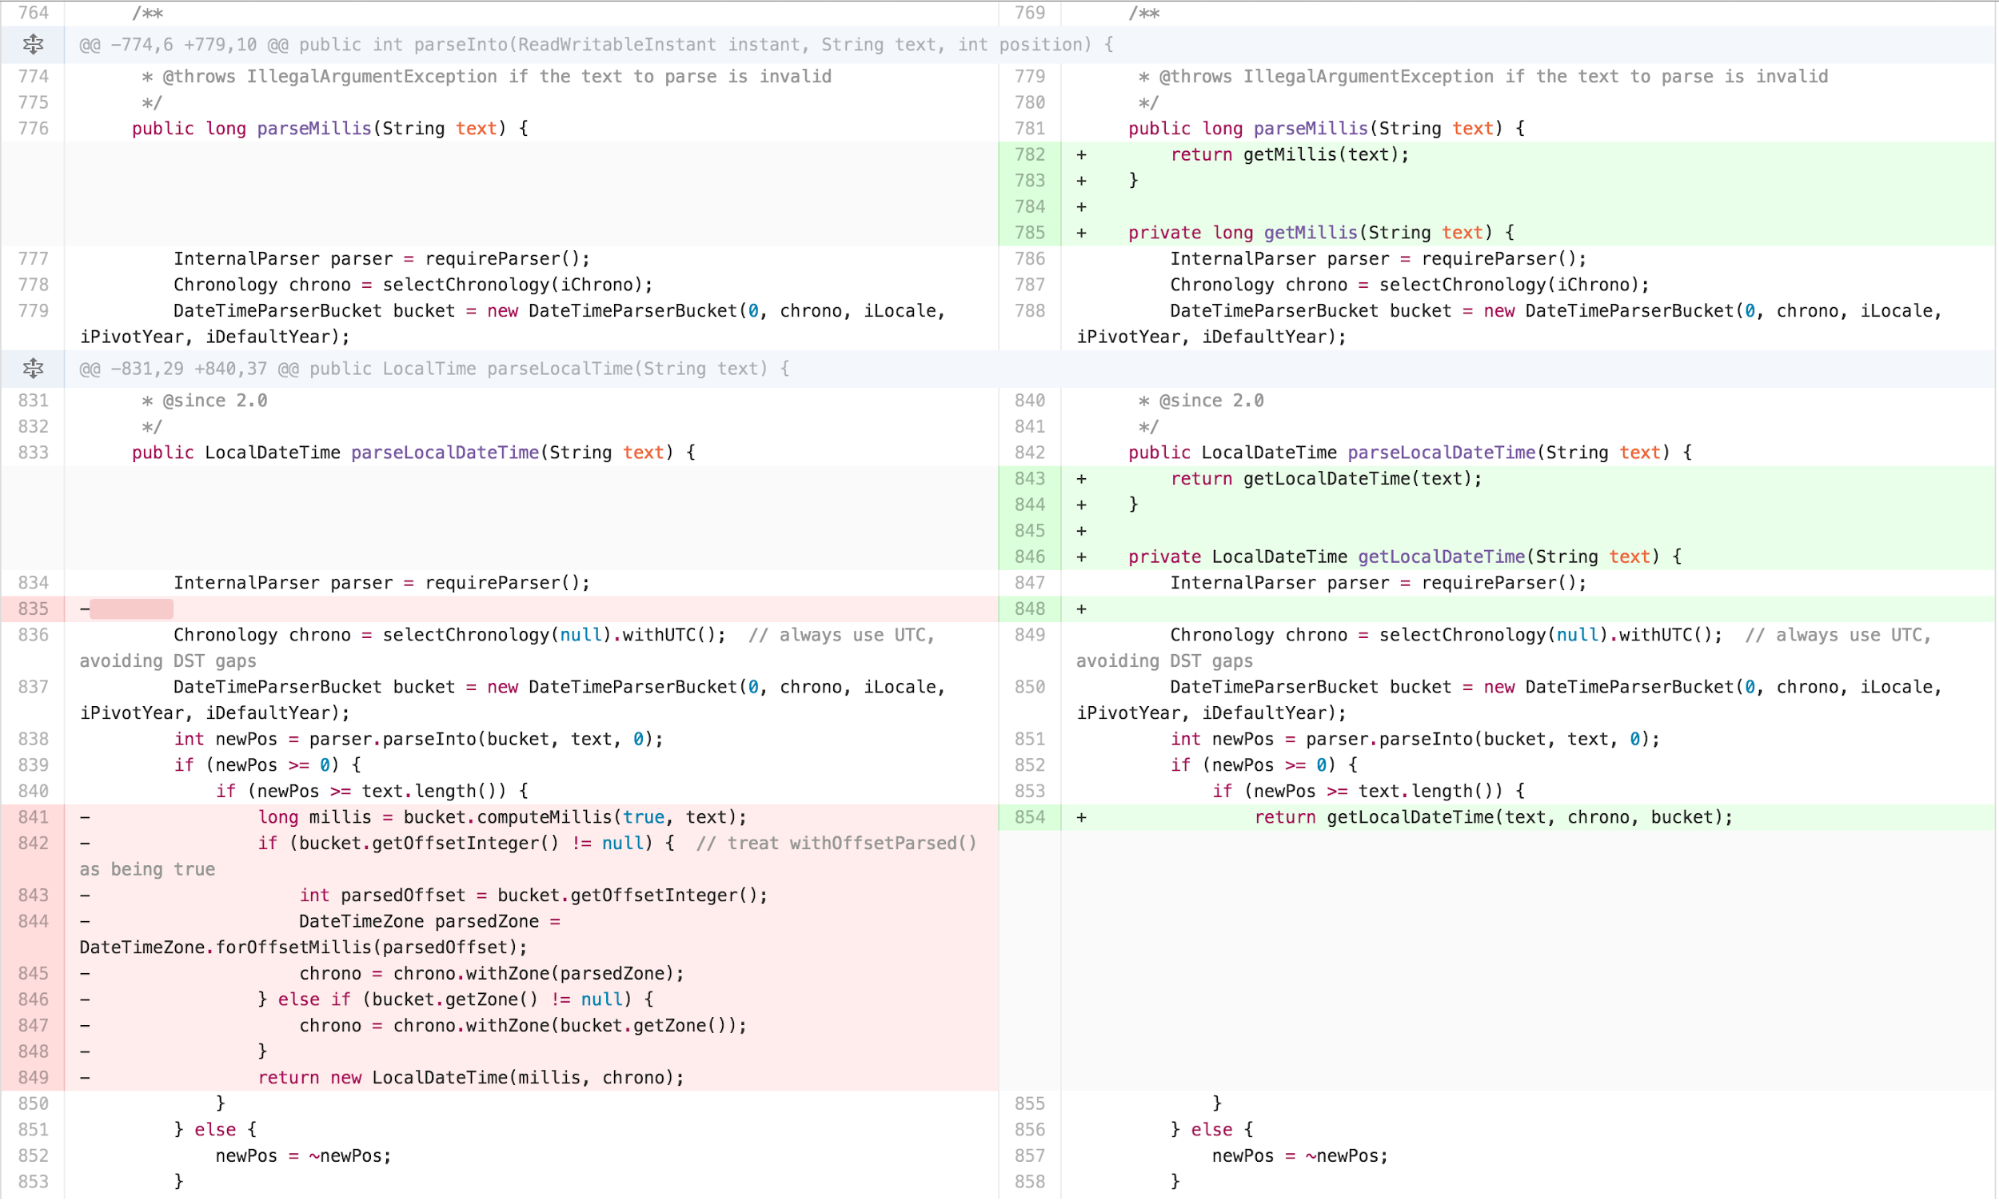
\includegraphics[width=\linewidth]{code38}
	\caption{insert caption}
\end{figure}
\begin{figure}[H]
	\centering
	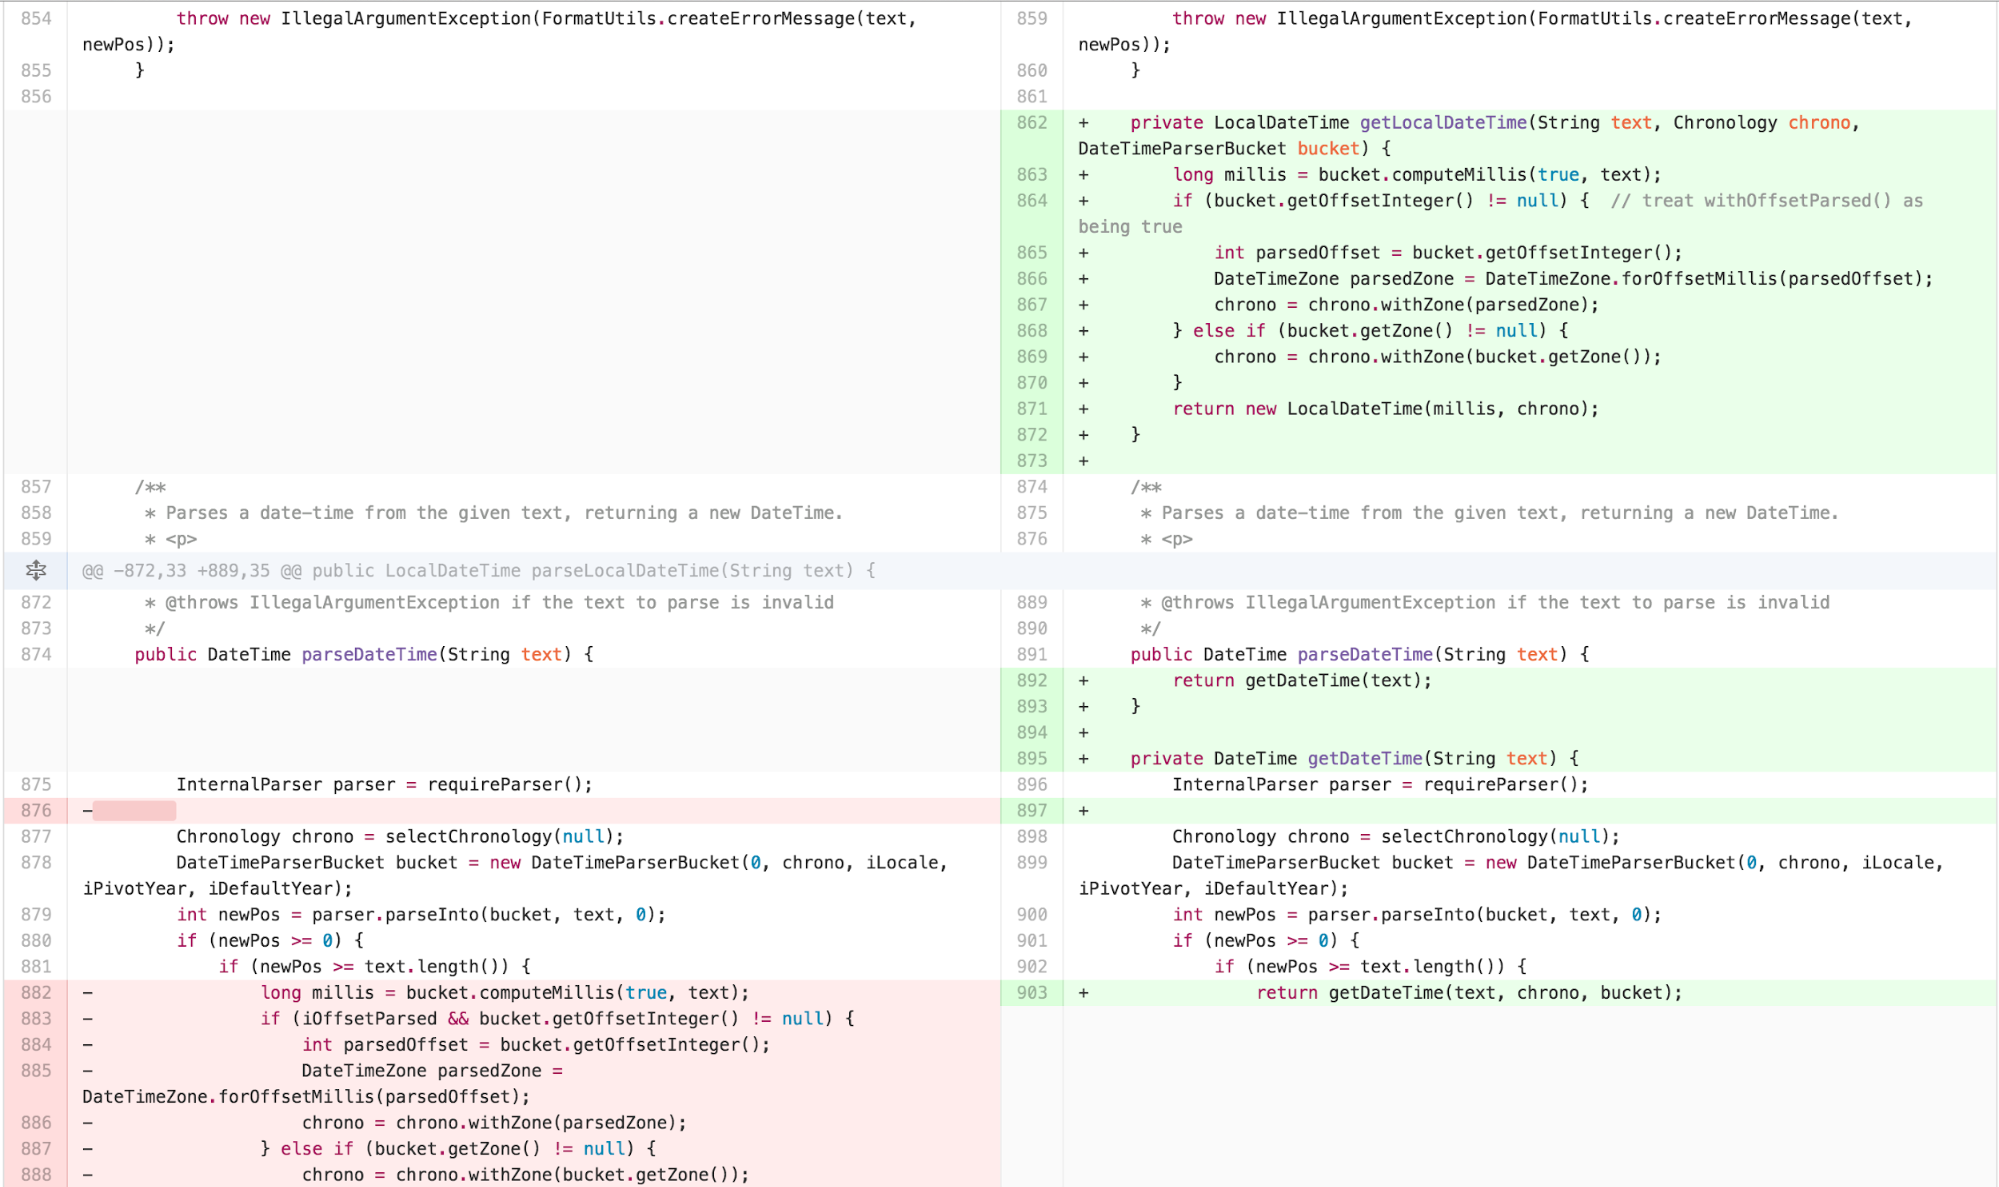
\includegraphics[width=\linewidth]{code39}
	\caption{insert caption}
\end{figure}
\begin{figure}[H]
	\centering
	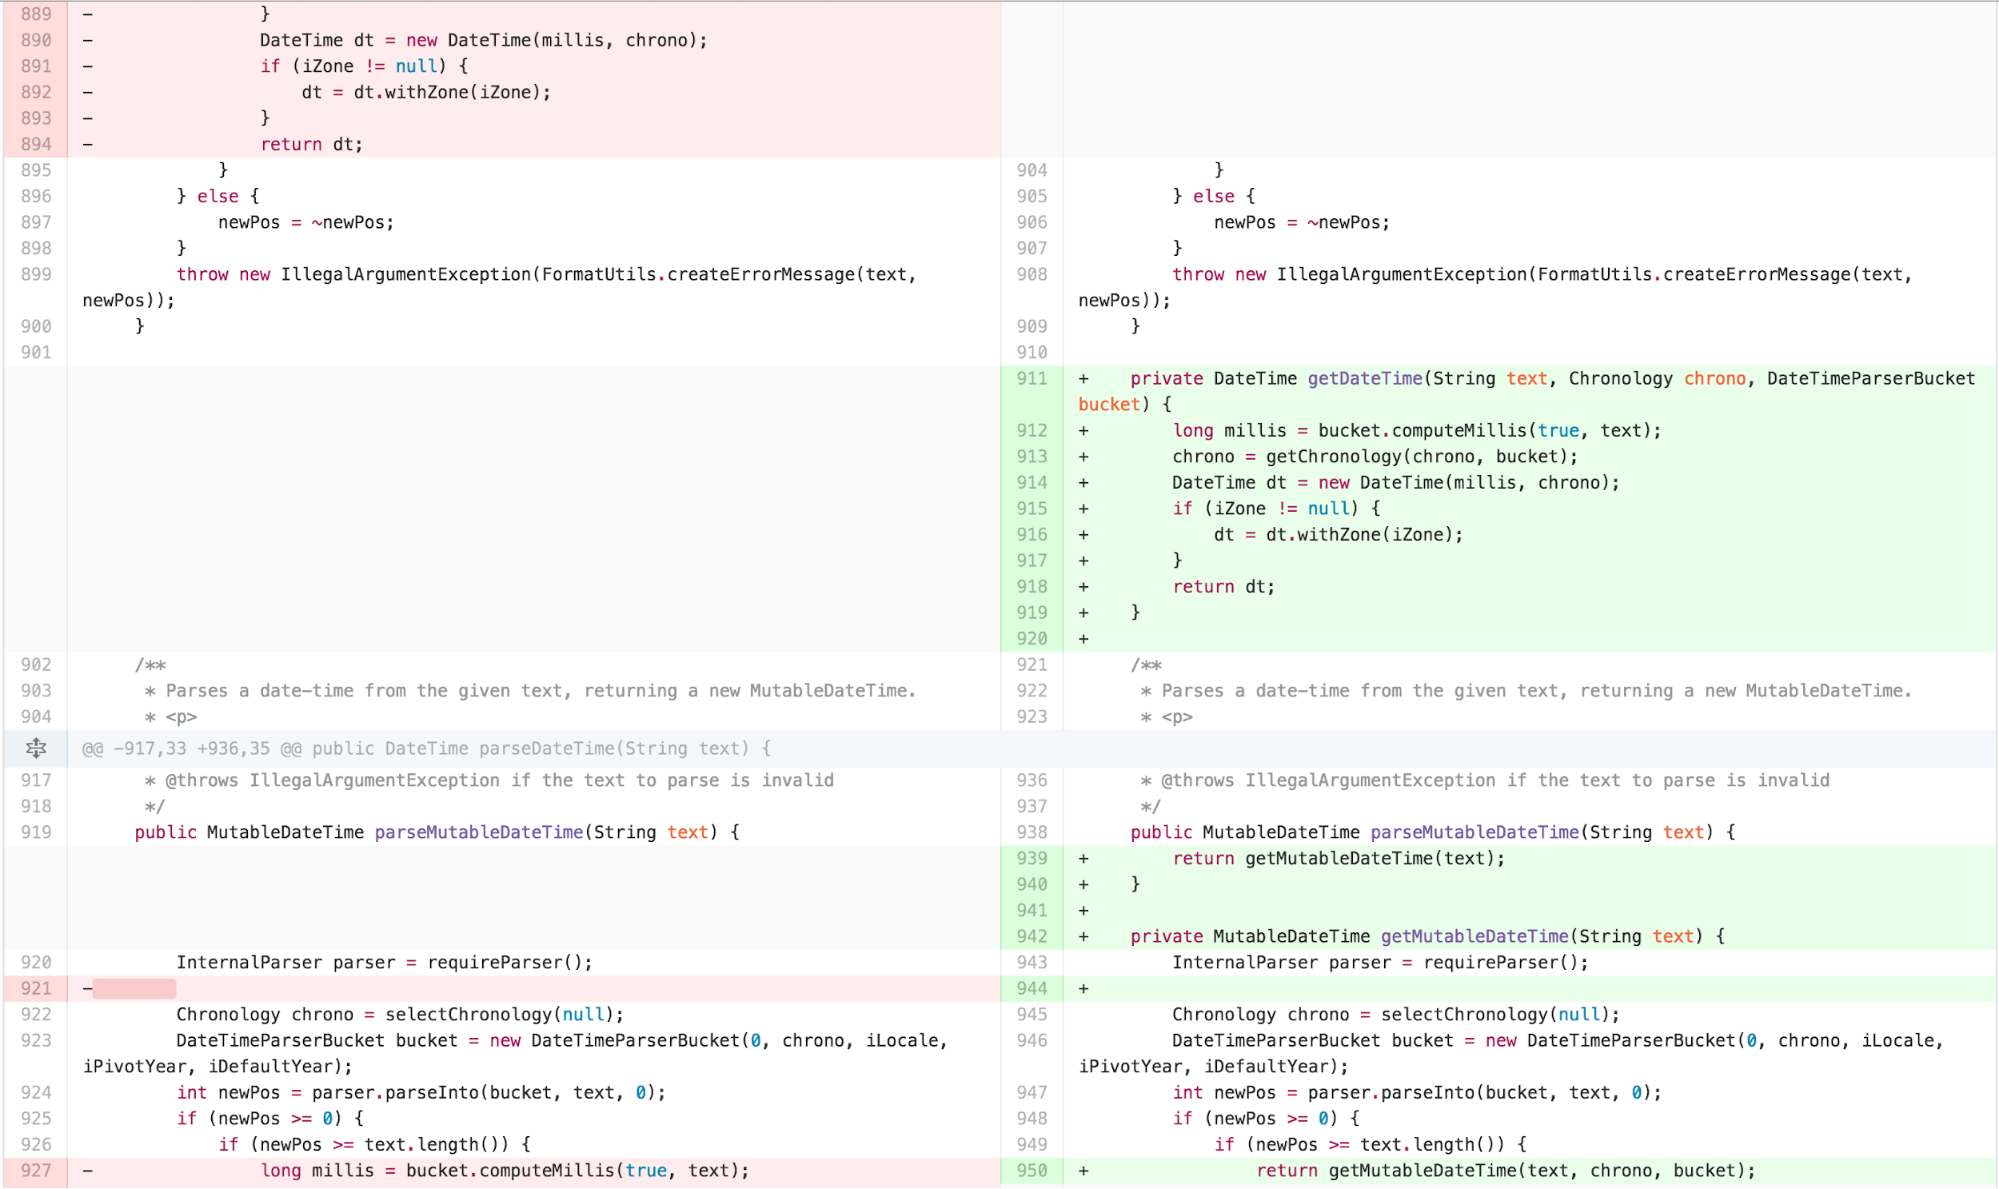
\includegraphics[width=\linewidth]{code40}
	\caption{insert caption}
\end{figure}
\begin{figure}[H]
	\centering
	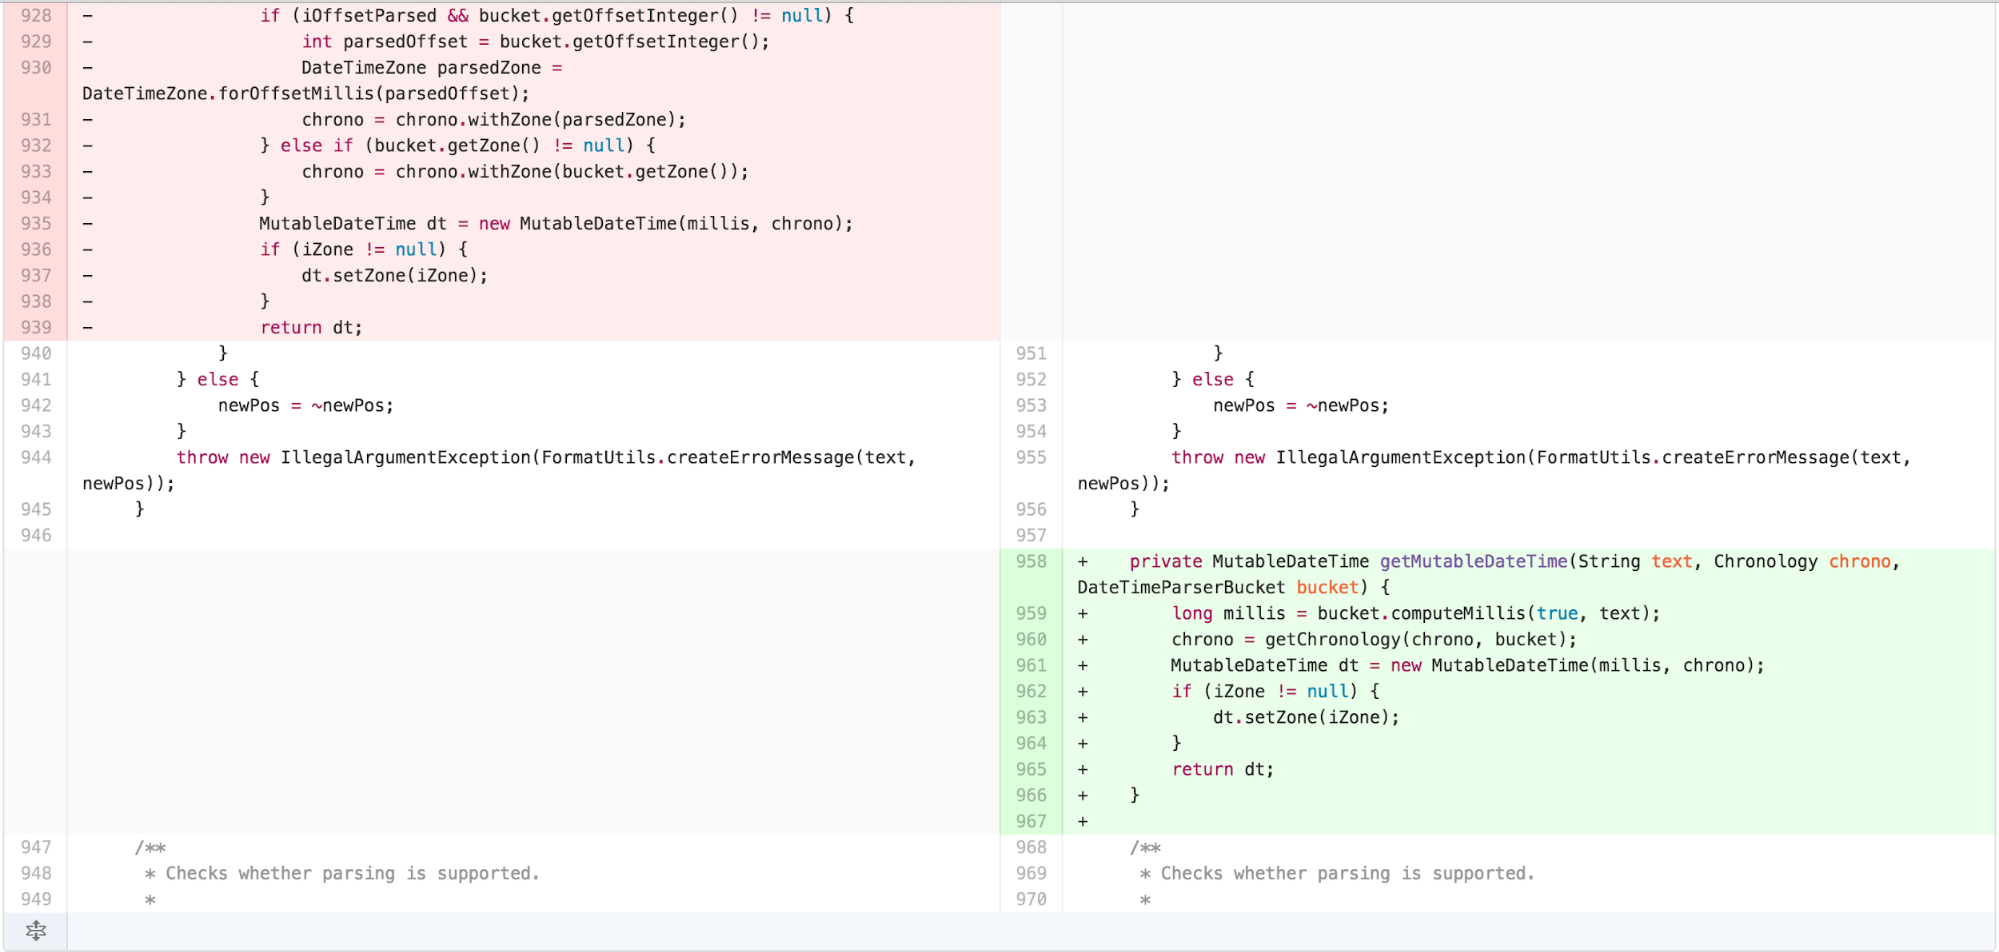
\includegraphics[width=\linewidth]{code41}
	\caption{insert caption}
\end{figure}

I then pushed the responsibility for \texttt{Chronology} calculation into a \texttt{ChronologyFactory}.

\begin{figure}[H]
	\centering
	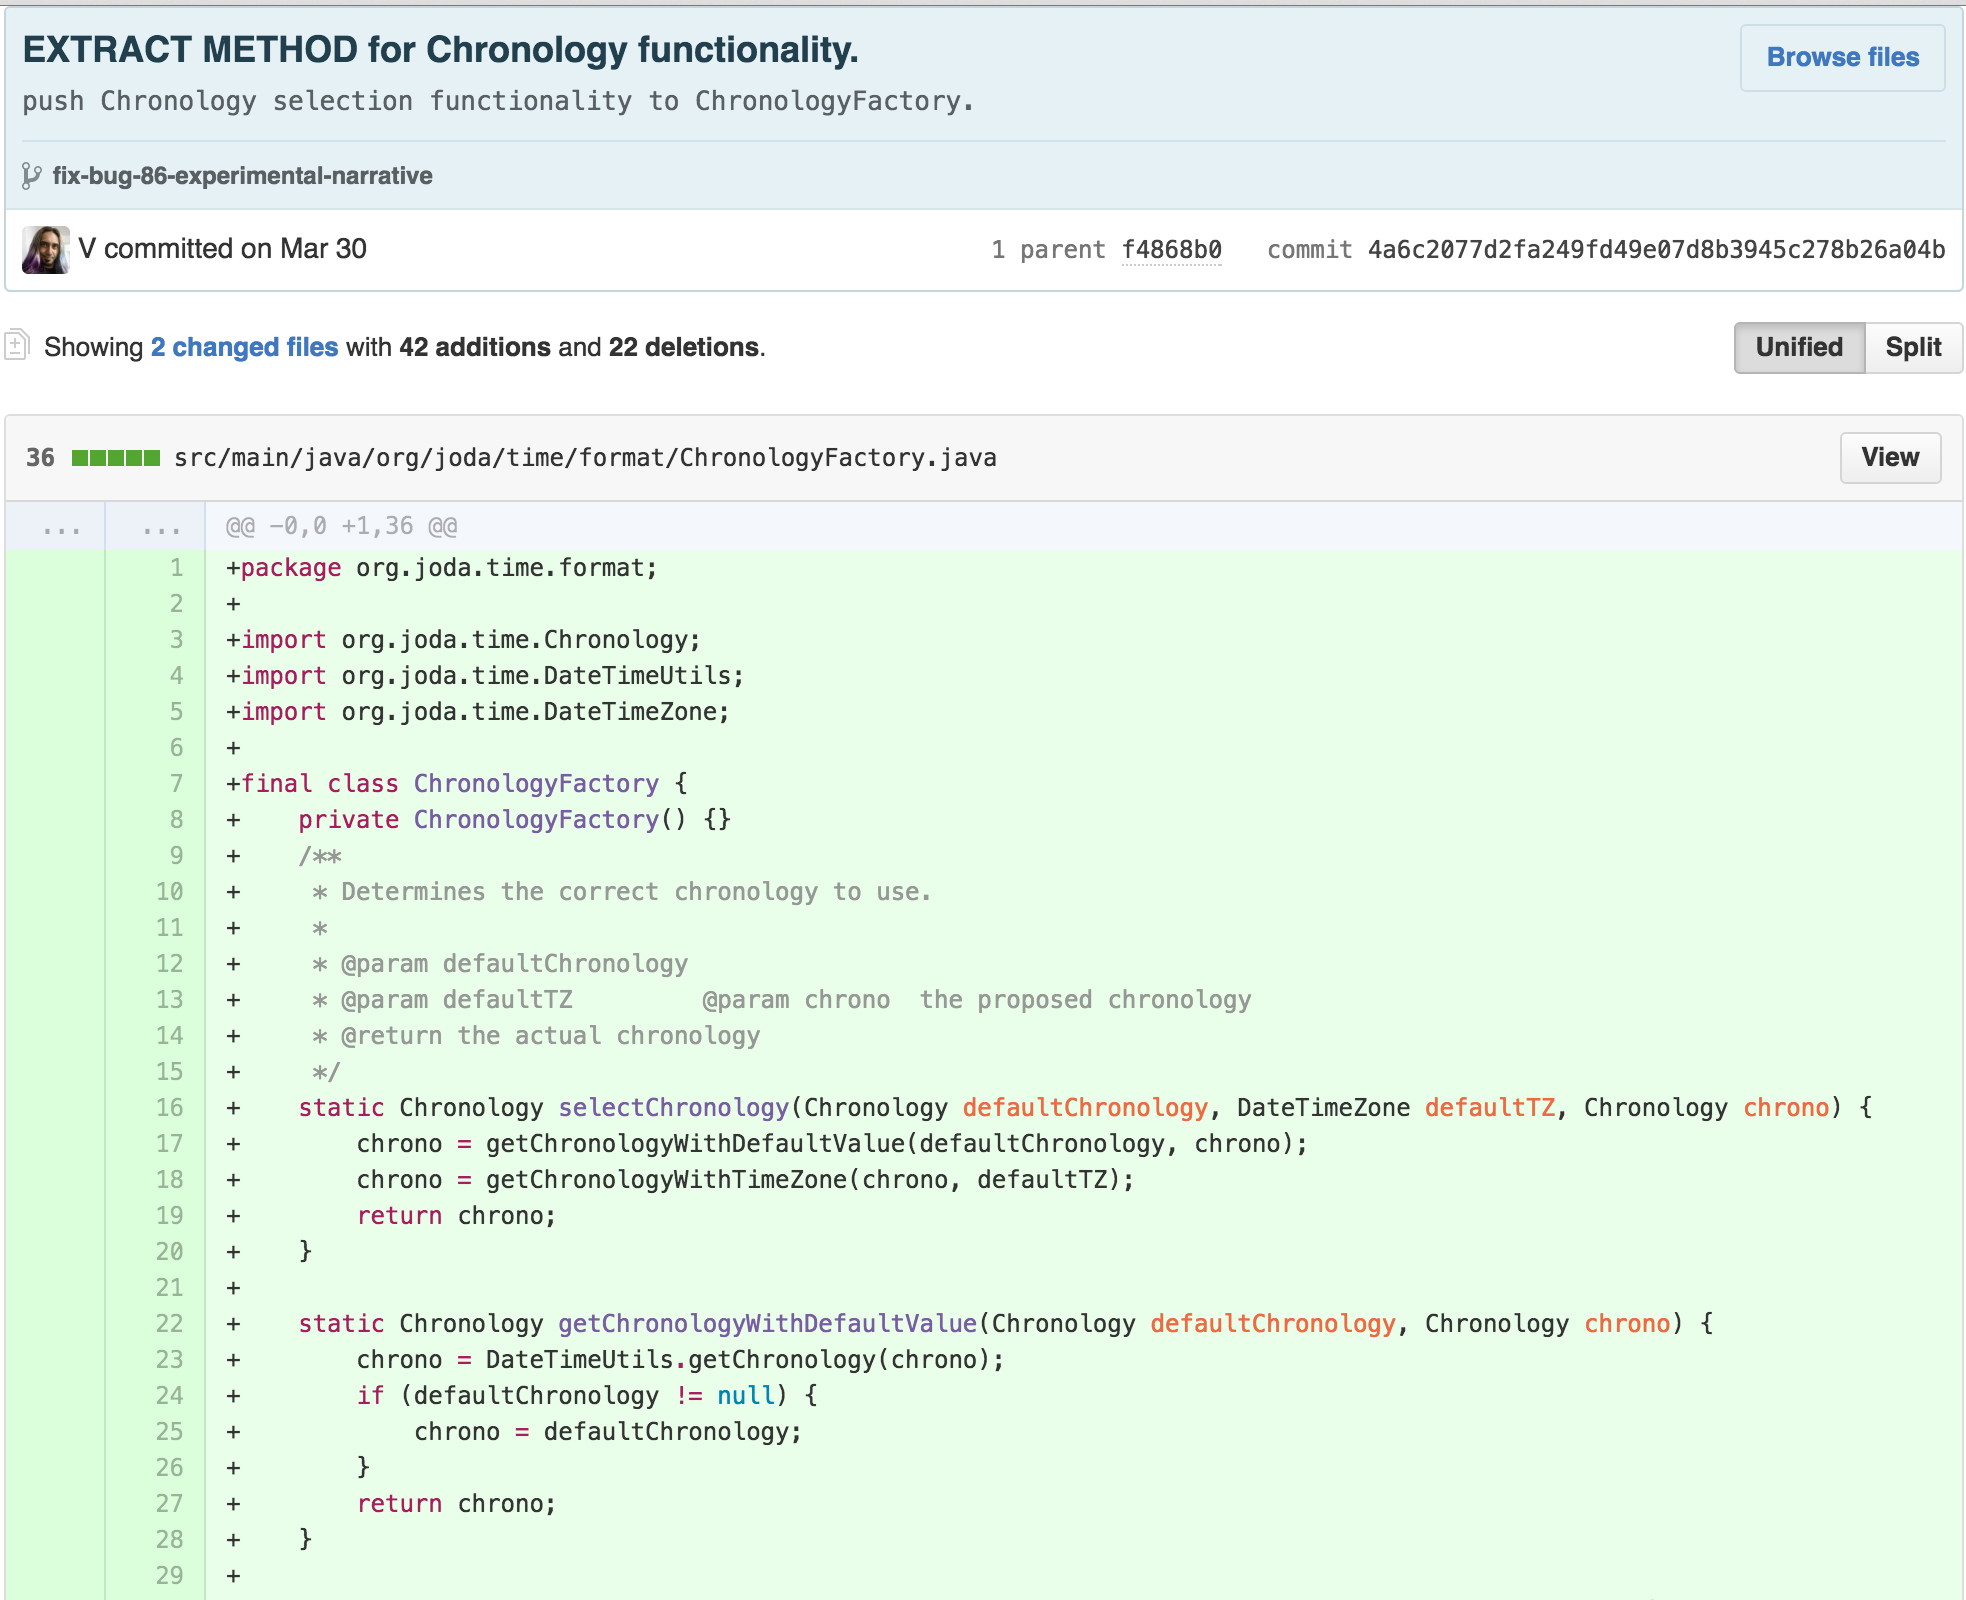
\includegraphics[width=\linewidth]{code42}
	\caption{insert caption}
\end{figure}
\begin{figure}[H]
	\centering
	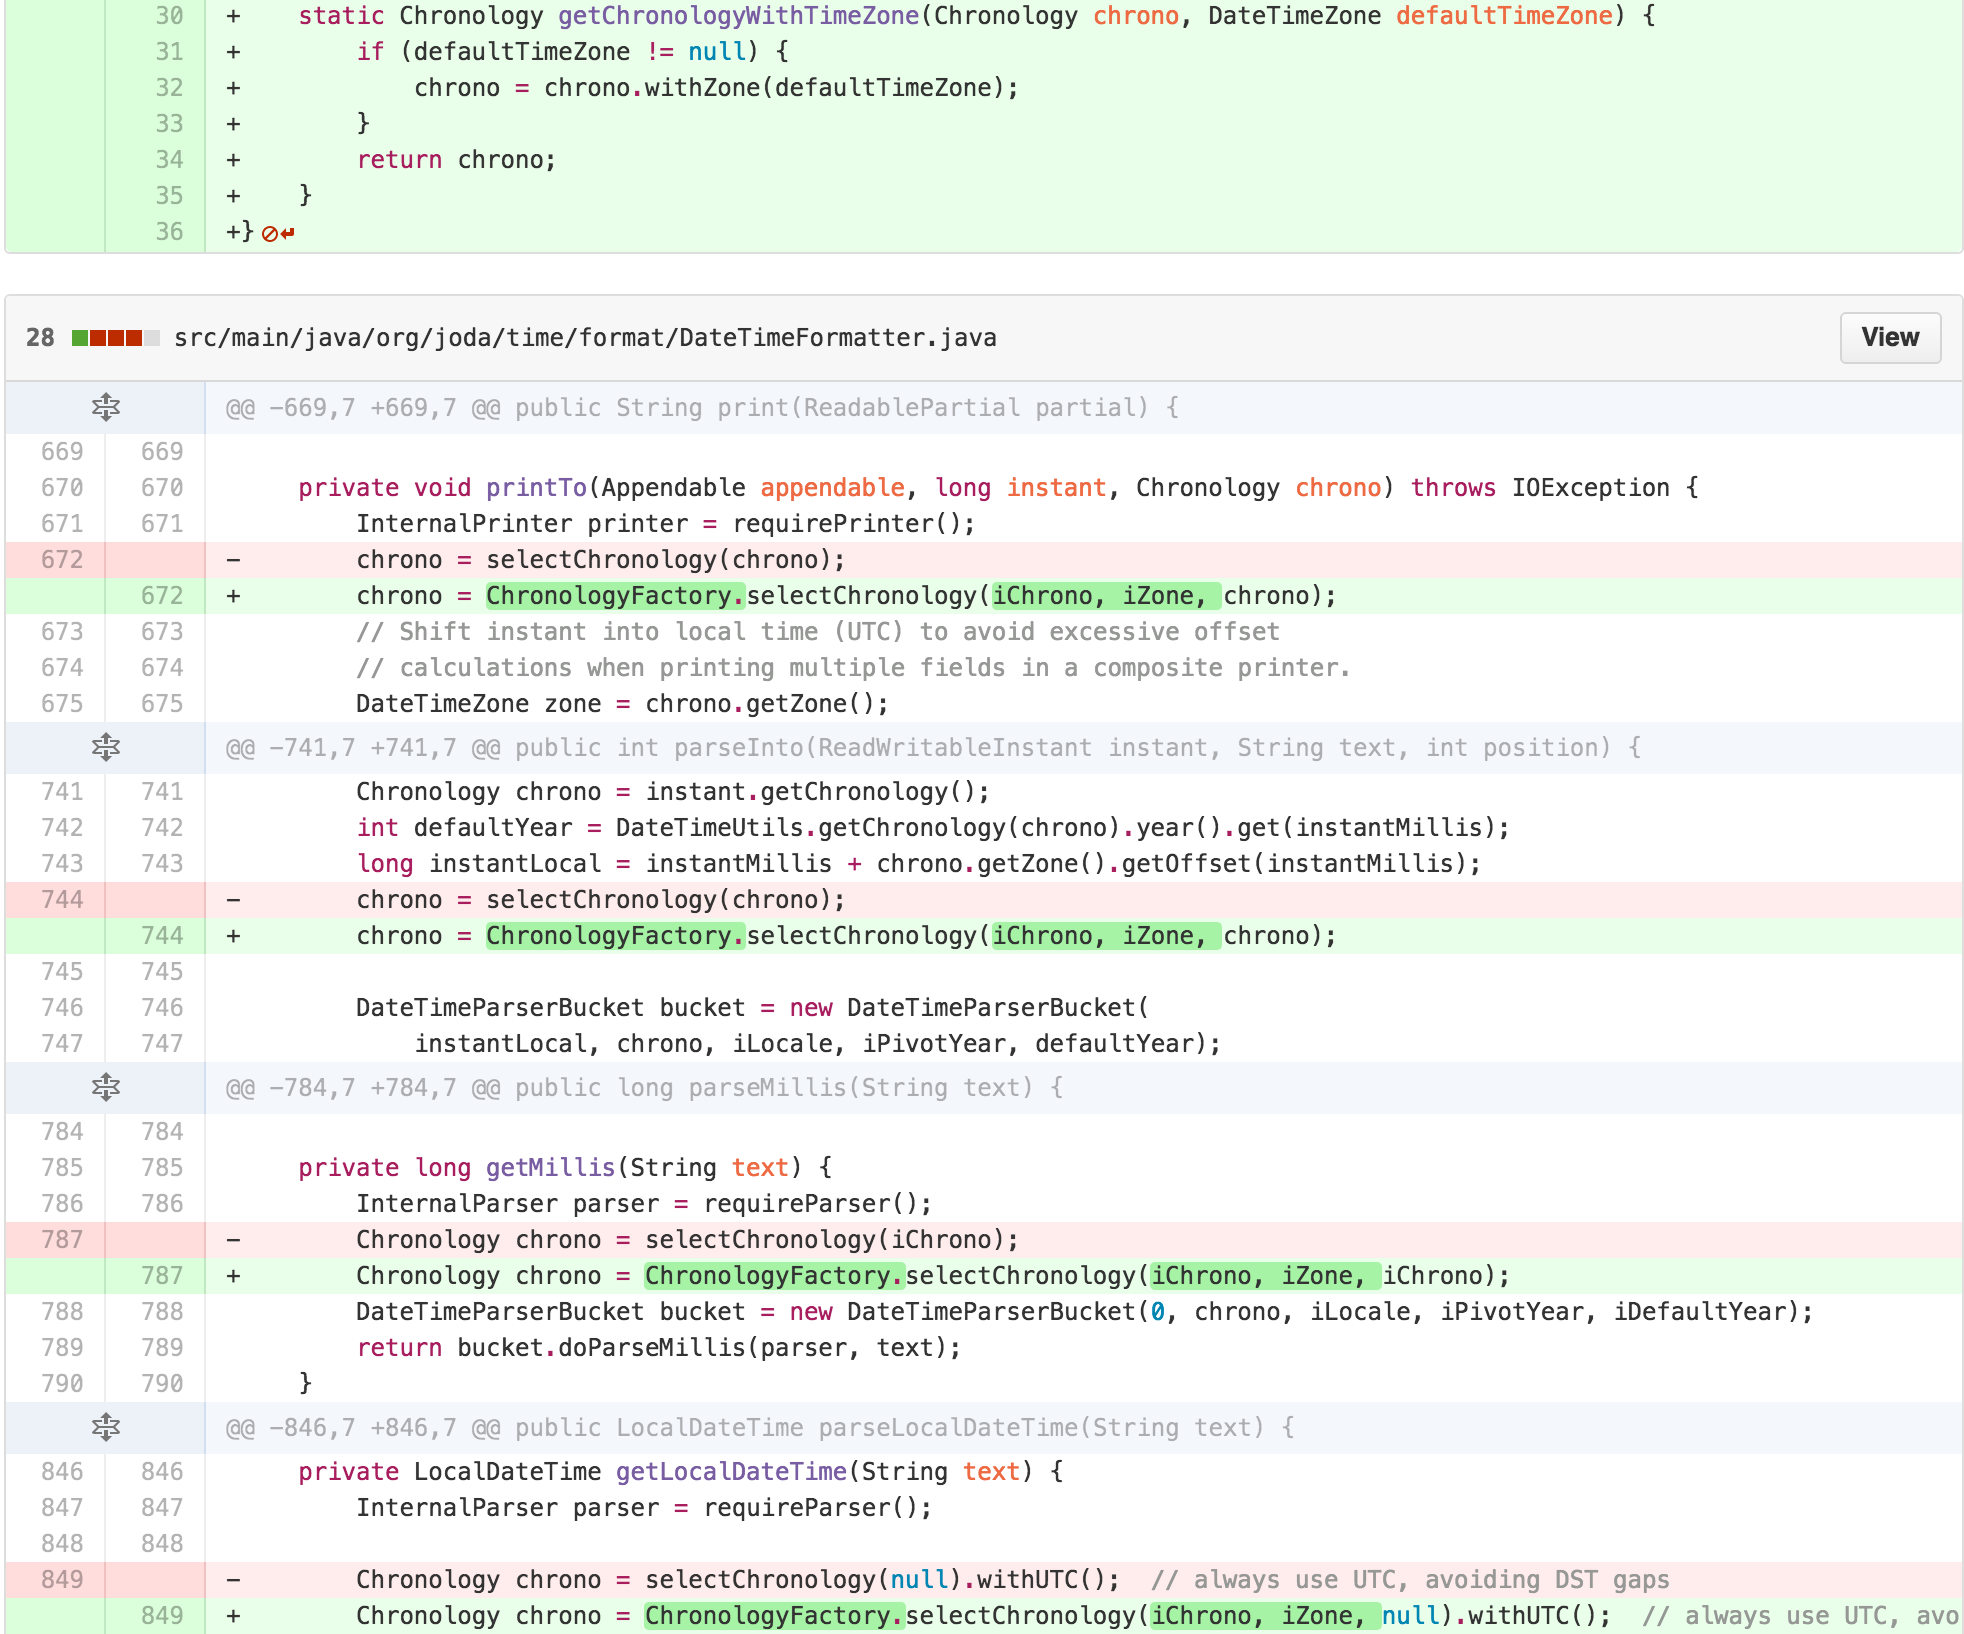
\includegraphics[width=\linewidth]{code43}
	\caption{insert caption}
\end{figure}
\begin{figure}[H]
	\centering
	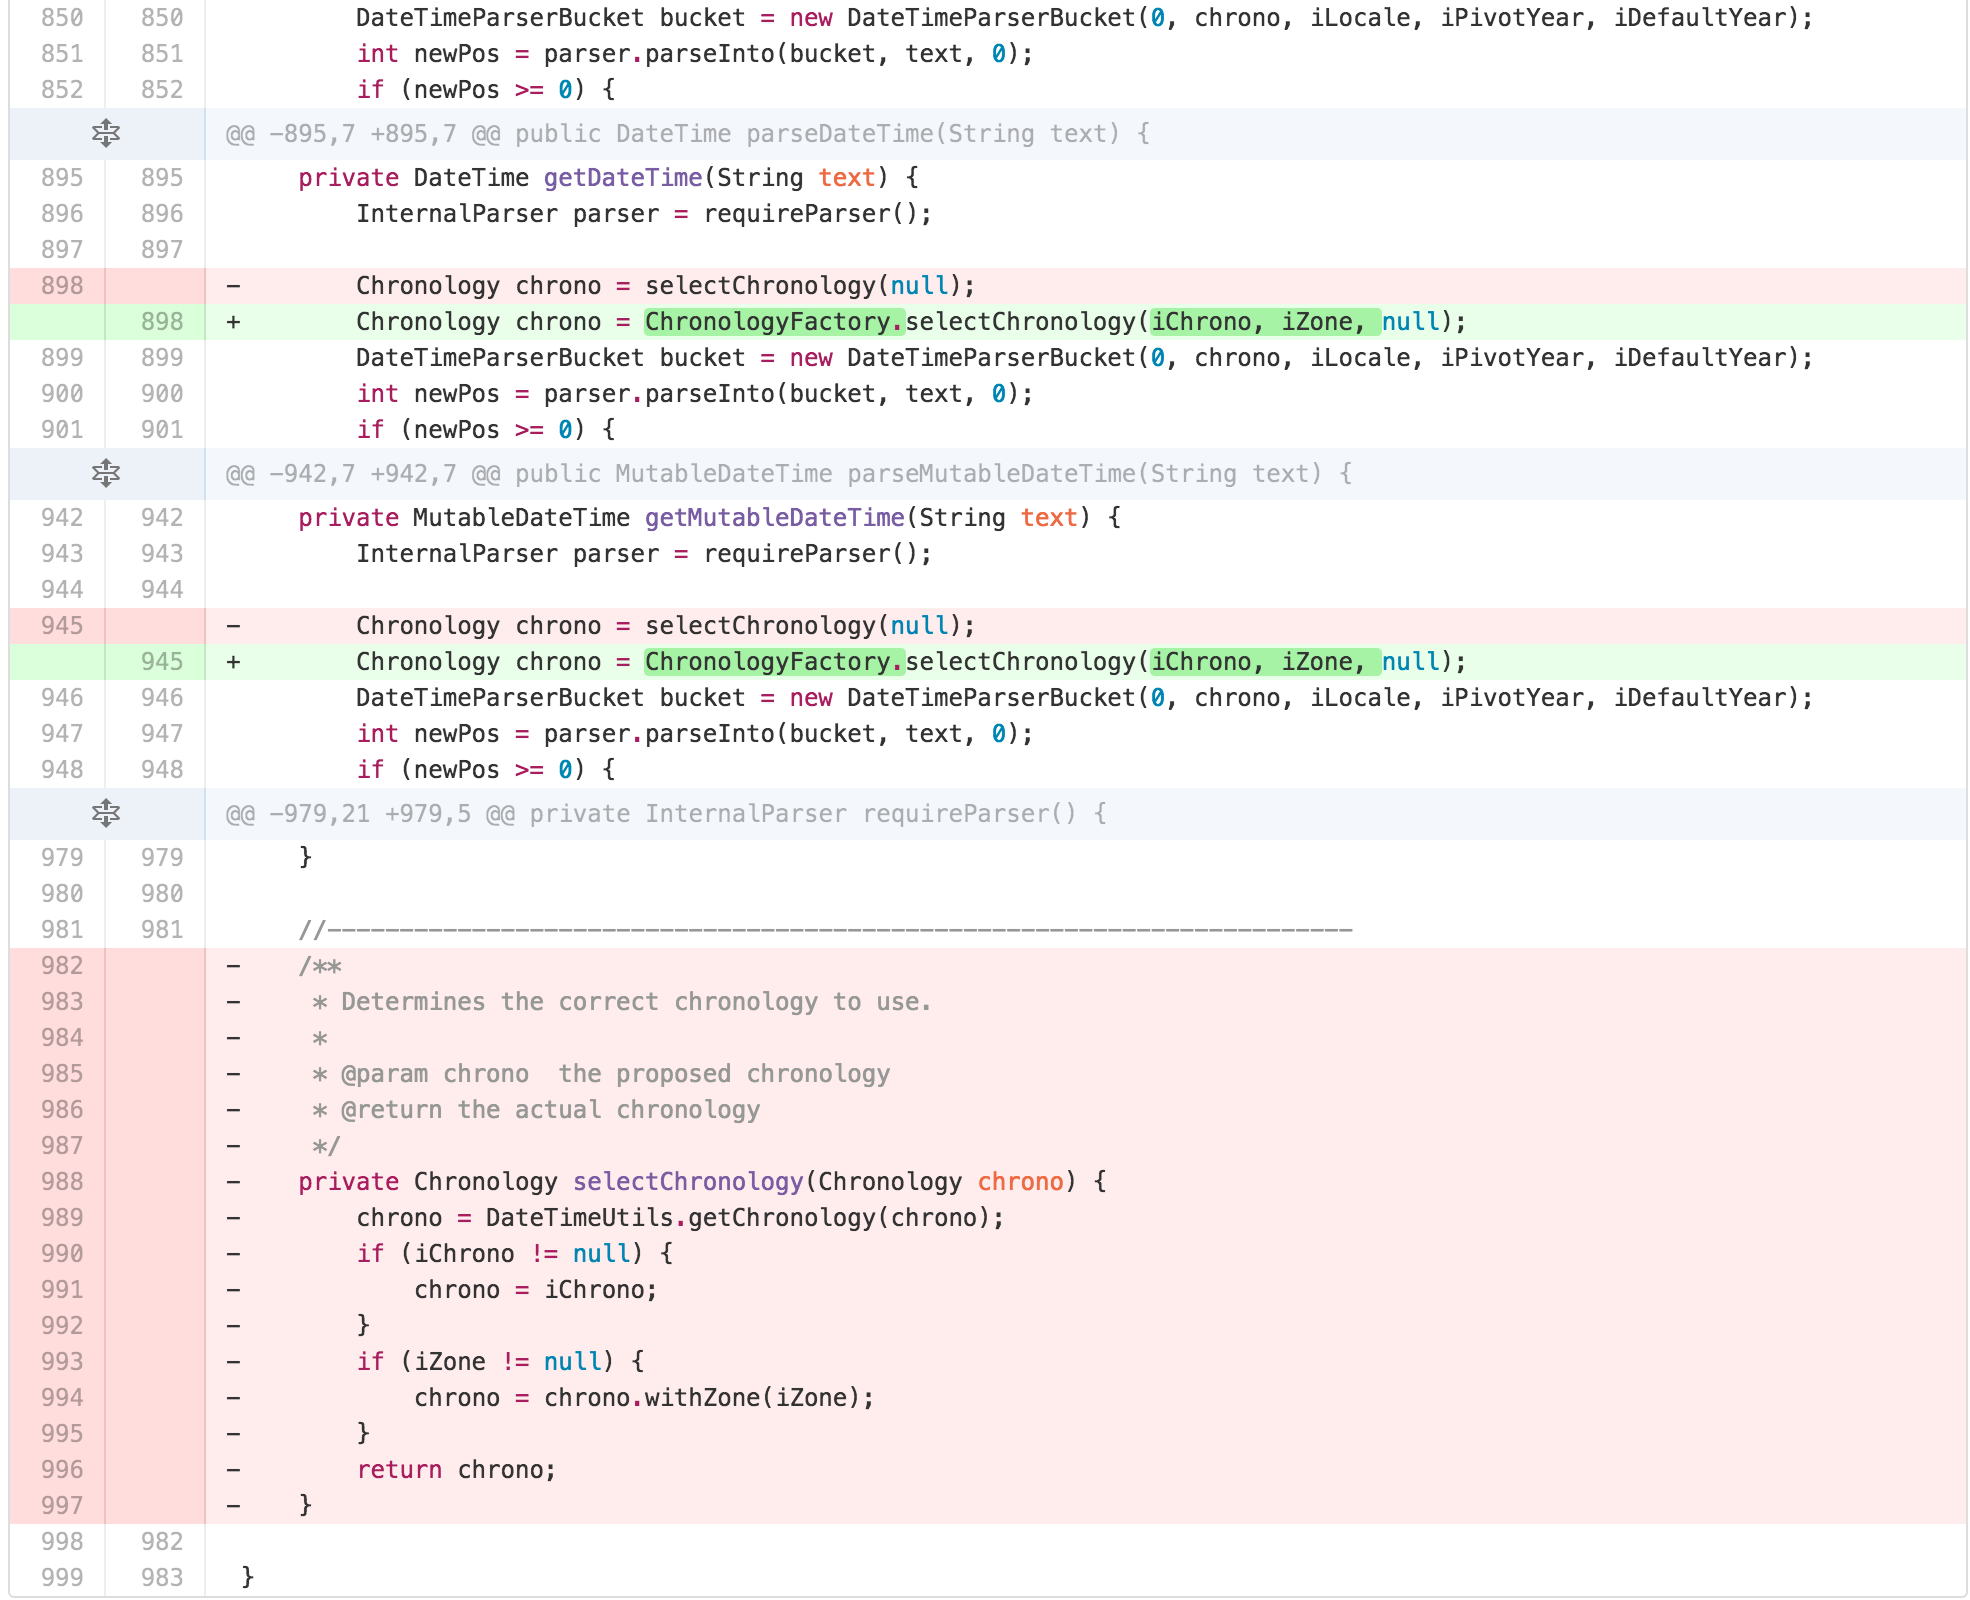
\includegraphics[width=\linewidth]{code44}
	\caption{insert caption}
\end{figure}
I then saw an opportunity. The similarity of the bodies of the \texttt{parseDateTime},  \texttt{parseLocalDateTime}, and \texttt{parseMutableDateTime} methods suggested to me that a TEMPLATE METHOD was hidden in this class. 

The use of a Design Pattern can increase the Germane Cognitive Load of an architecture, which can be more difficult for novices to understand. However, application of this pattern here likely resulted in a dramatically simpler \texttt{DateTimeFormatter} and better coherence in the architecture. Following Guideline 25: Write High Coherent Texts for Low Knowledge Readers, this strategic use of a design pattern seemed likely to make the code easier to understand for novices as well. Hence, I started working to make this pattern manifest. Through a series of commits, I realized that \texttt{DateTimeFormatter} had a lot of FEATURE ENVY with \texttt{DateTimeParserBucket}.

\begin{figure}[H]
	\centering
	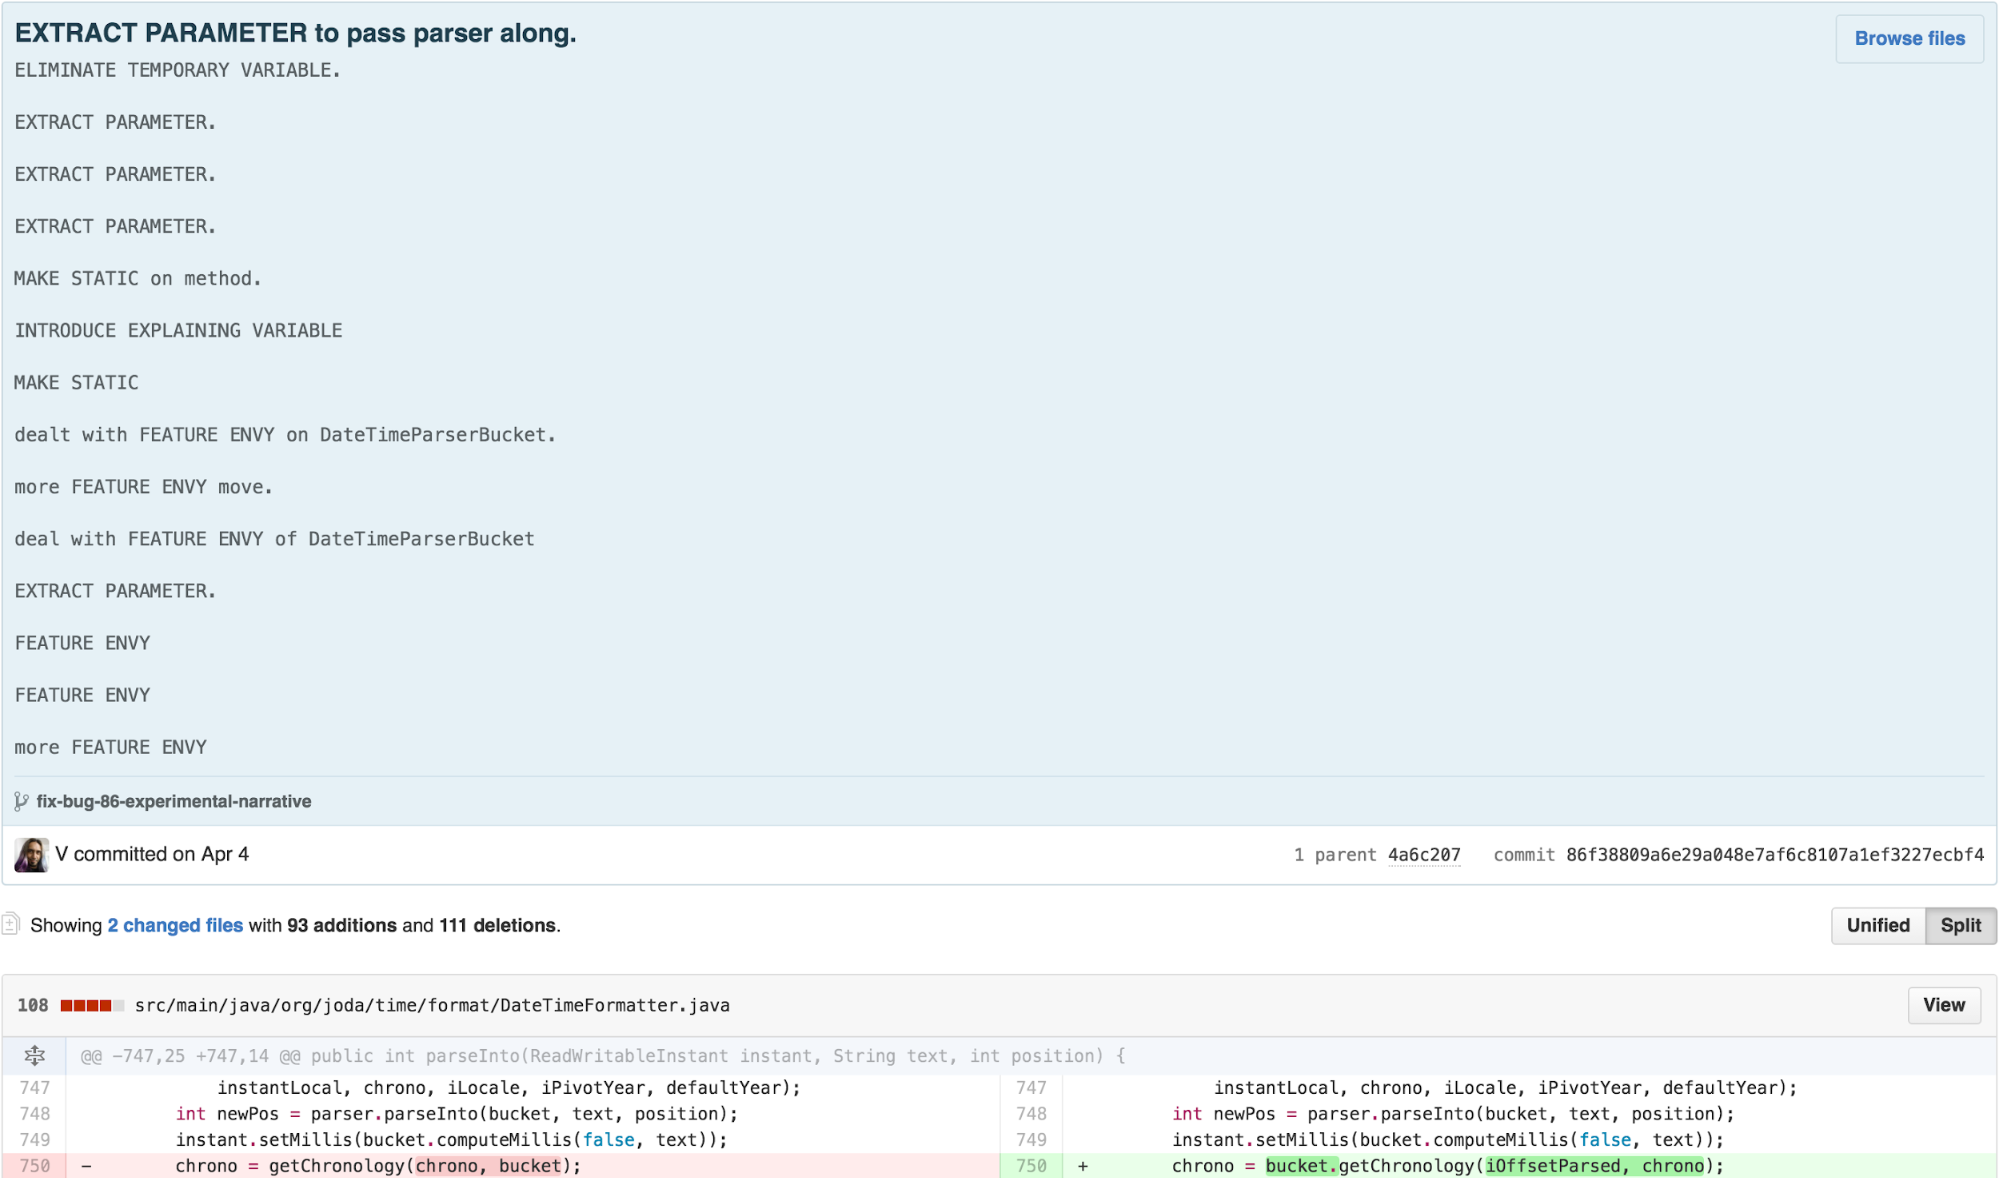
\includegraphics[width=\linewidth]{code45}
	\caption{insert caption}
\end{figure}
\begin{figure}[H]
	\centering
	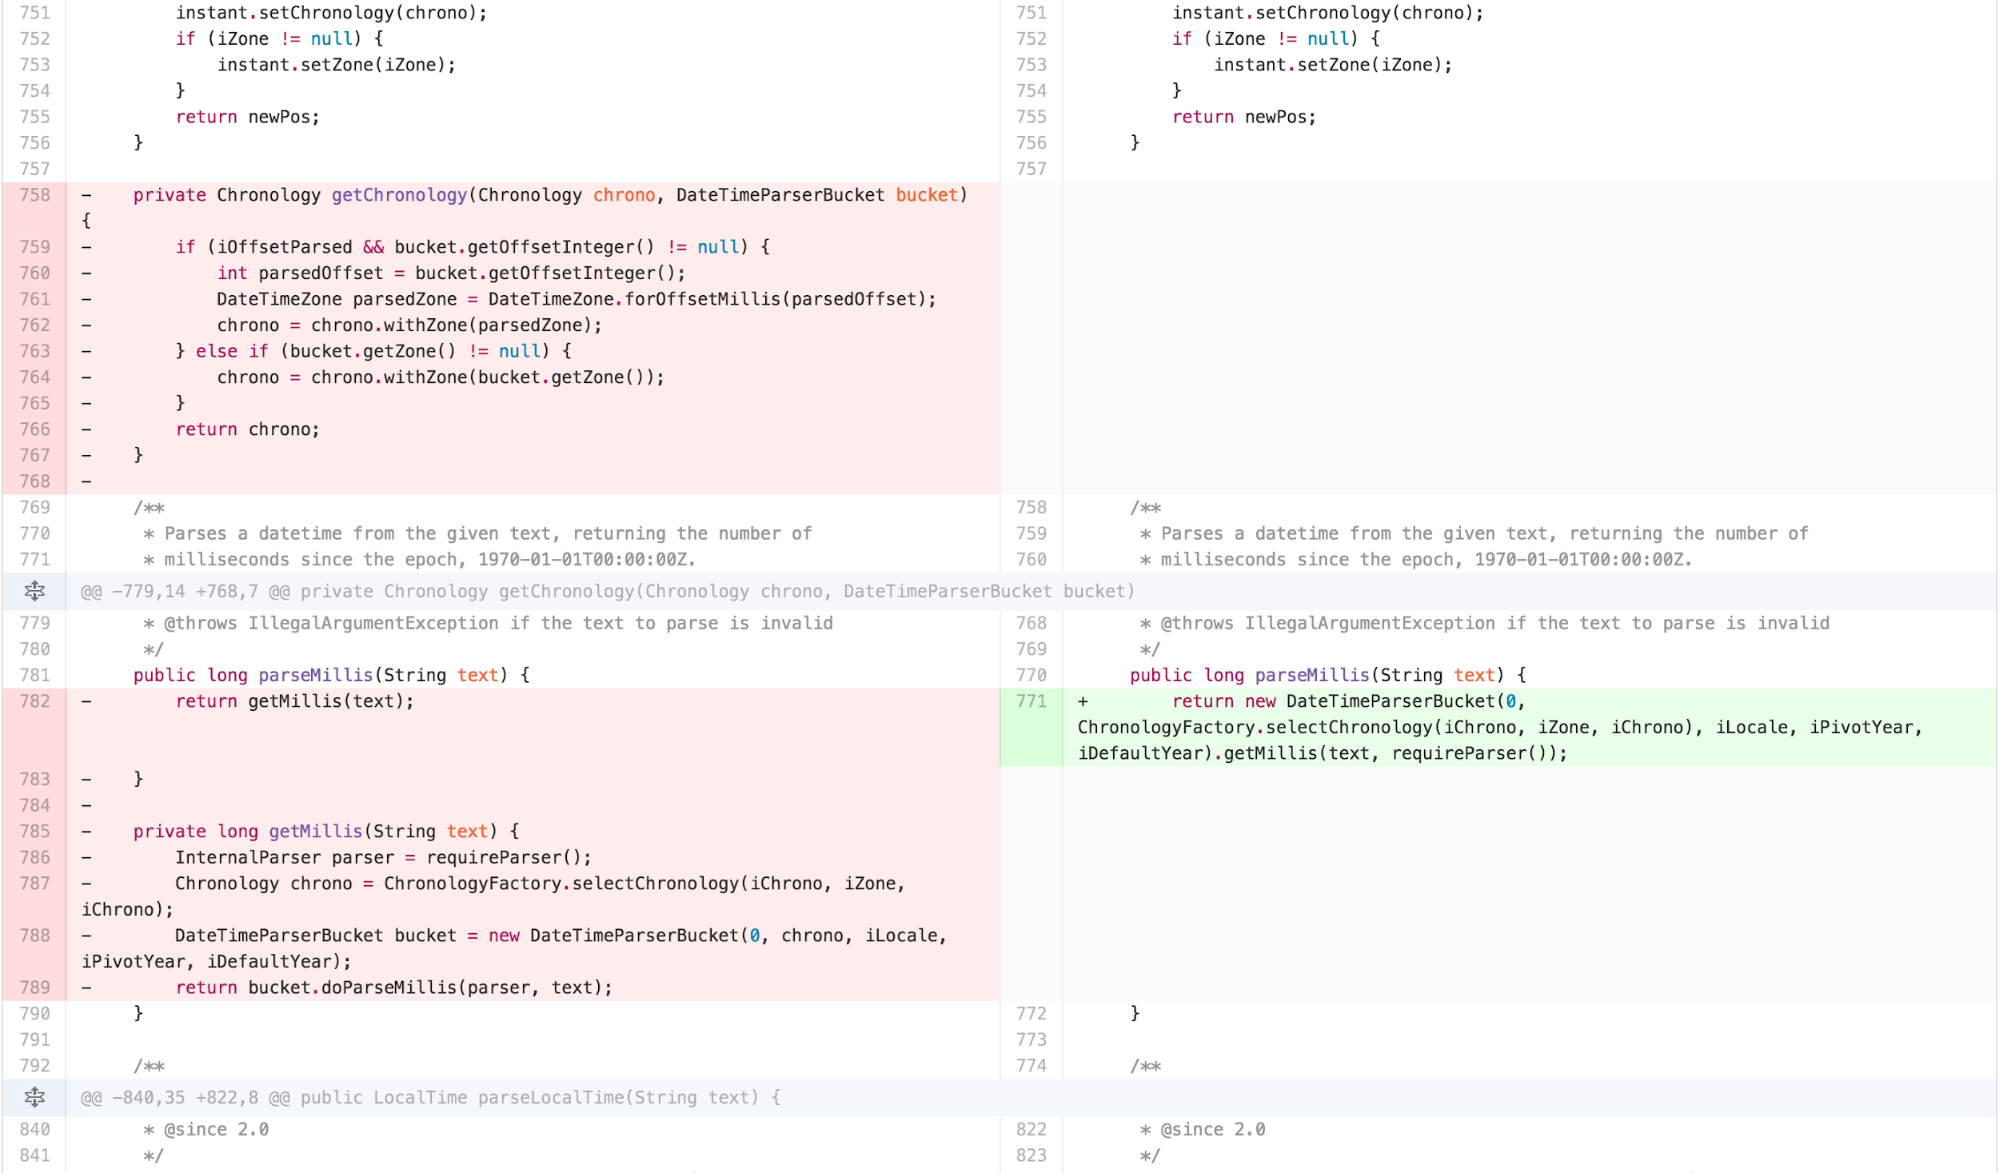
\includegraphics[width=\linewidth]{code46}
	\caption{insert caption}
\end{figure}
\begin{figure}[H]
	\centering
	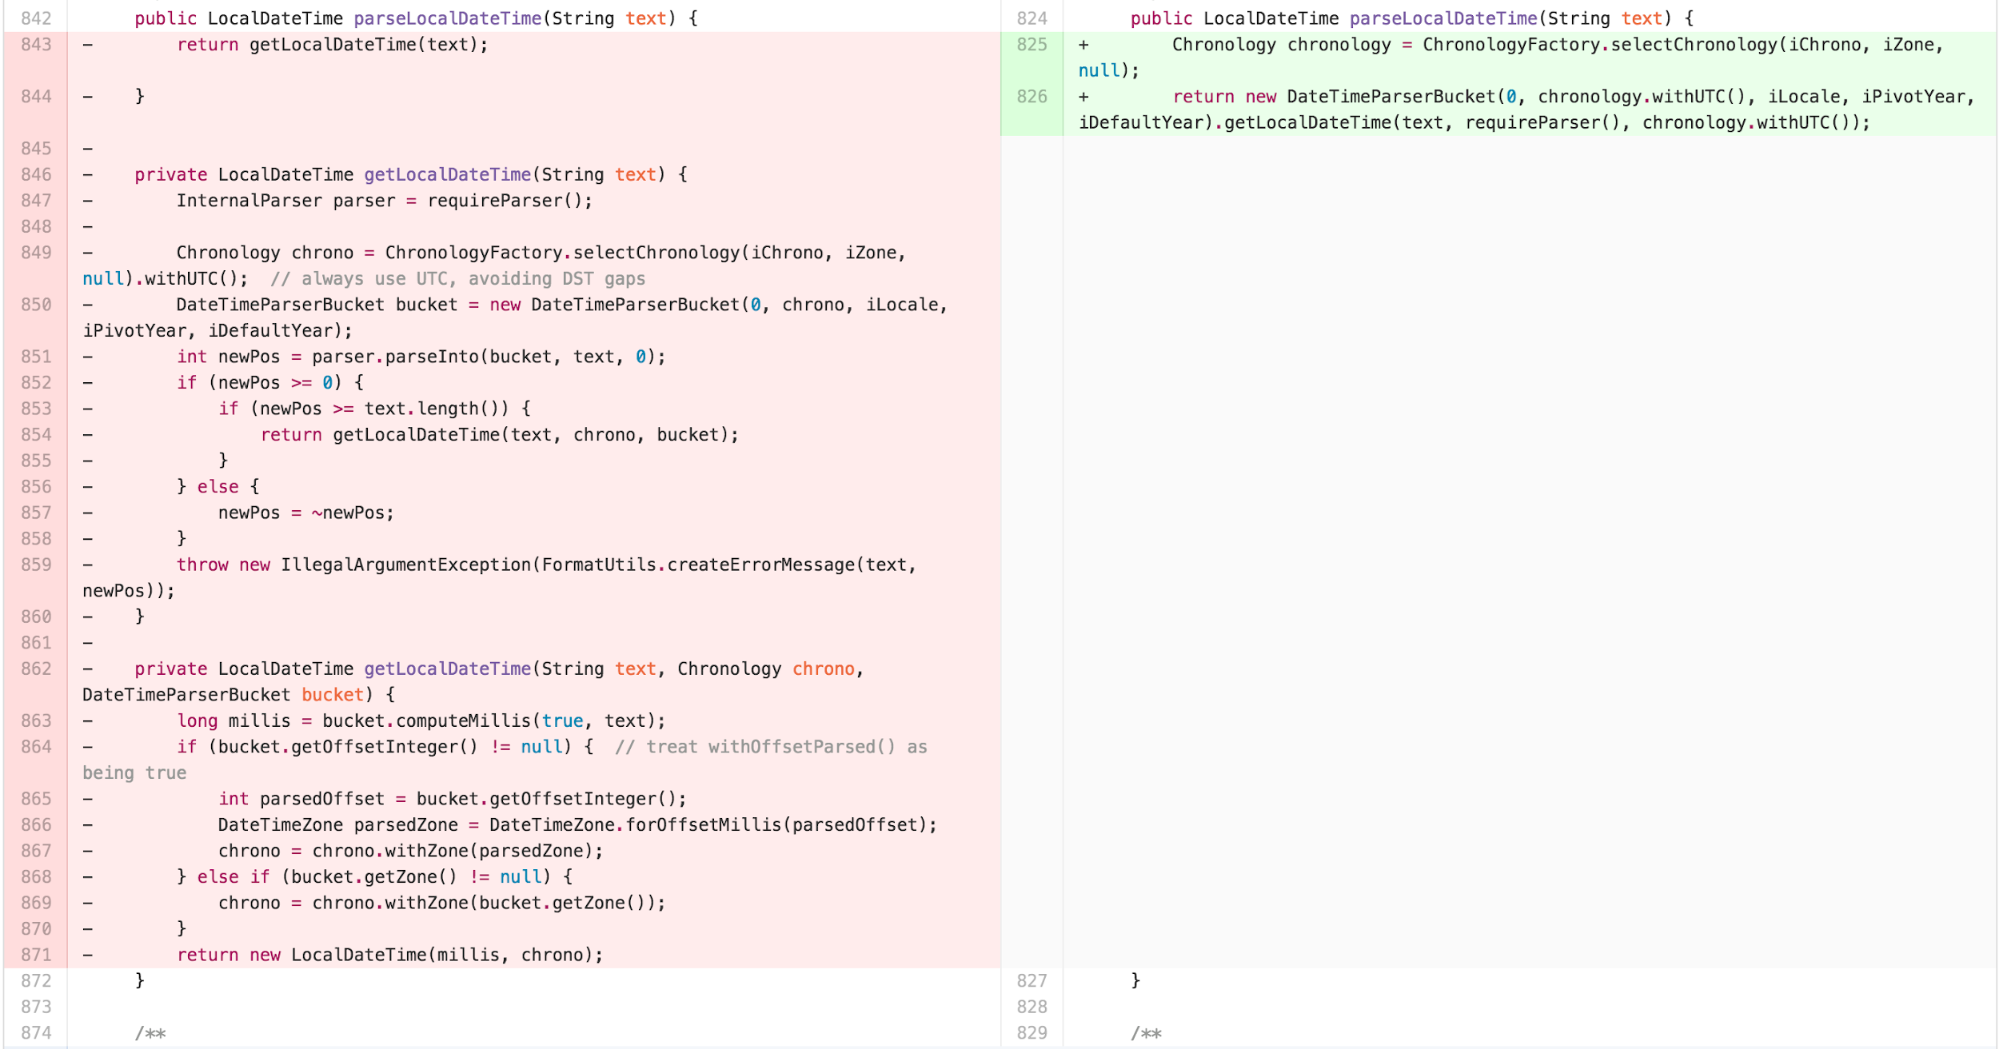
\includegraphics[width=\linewidth]{code47}
	\caption{insert caption}
\end{figure}
\begin{figure}[H]
	\centering
	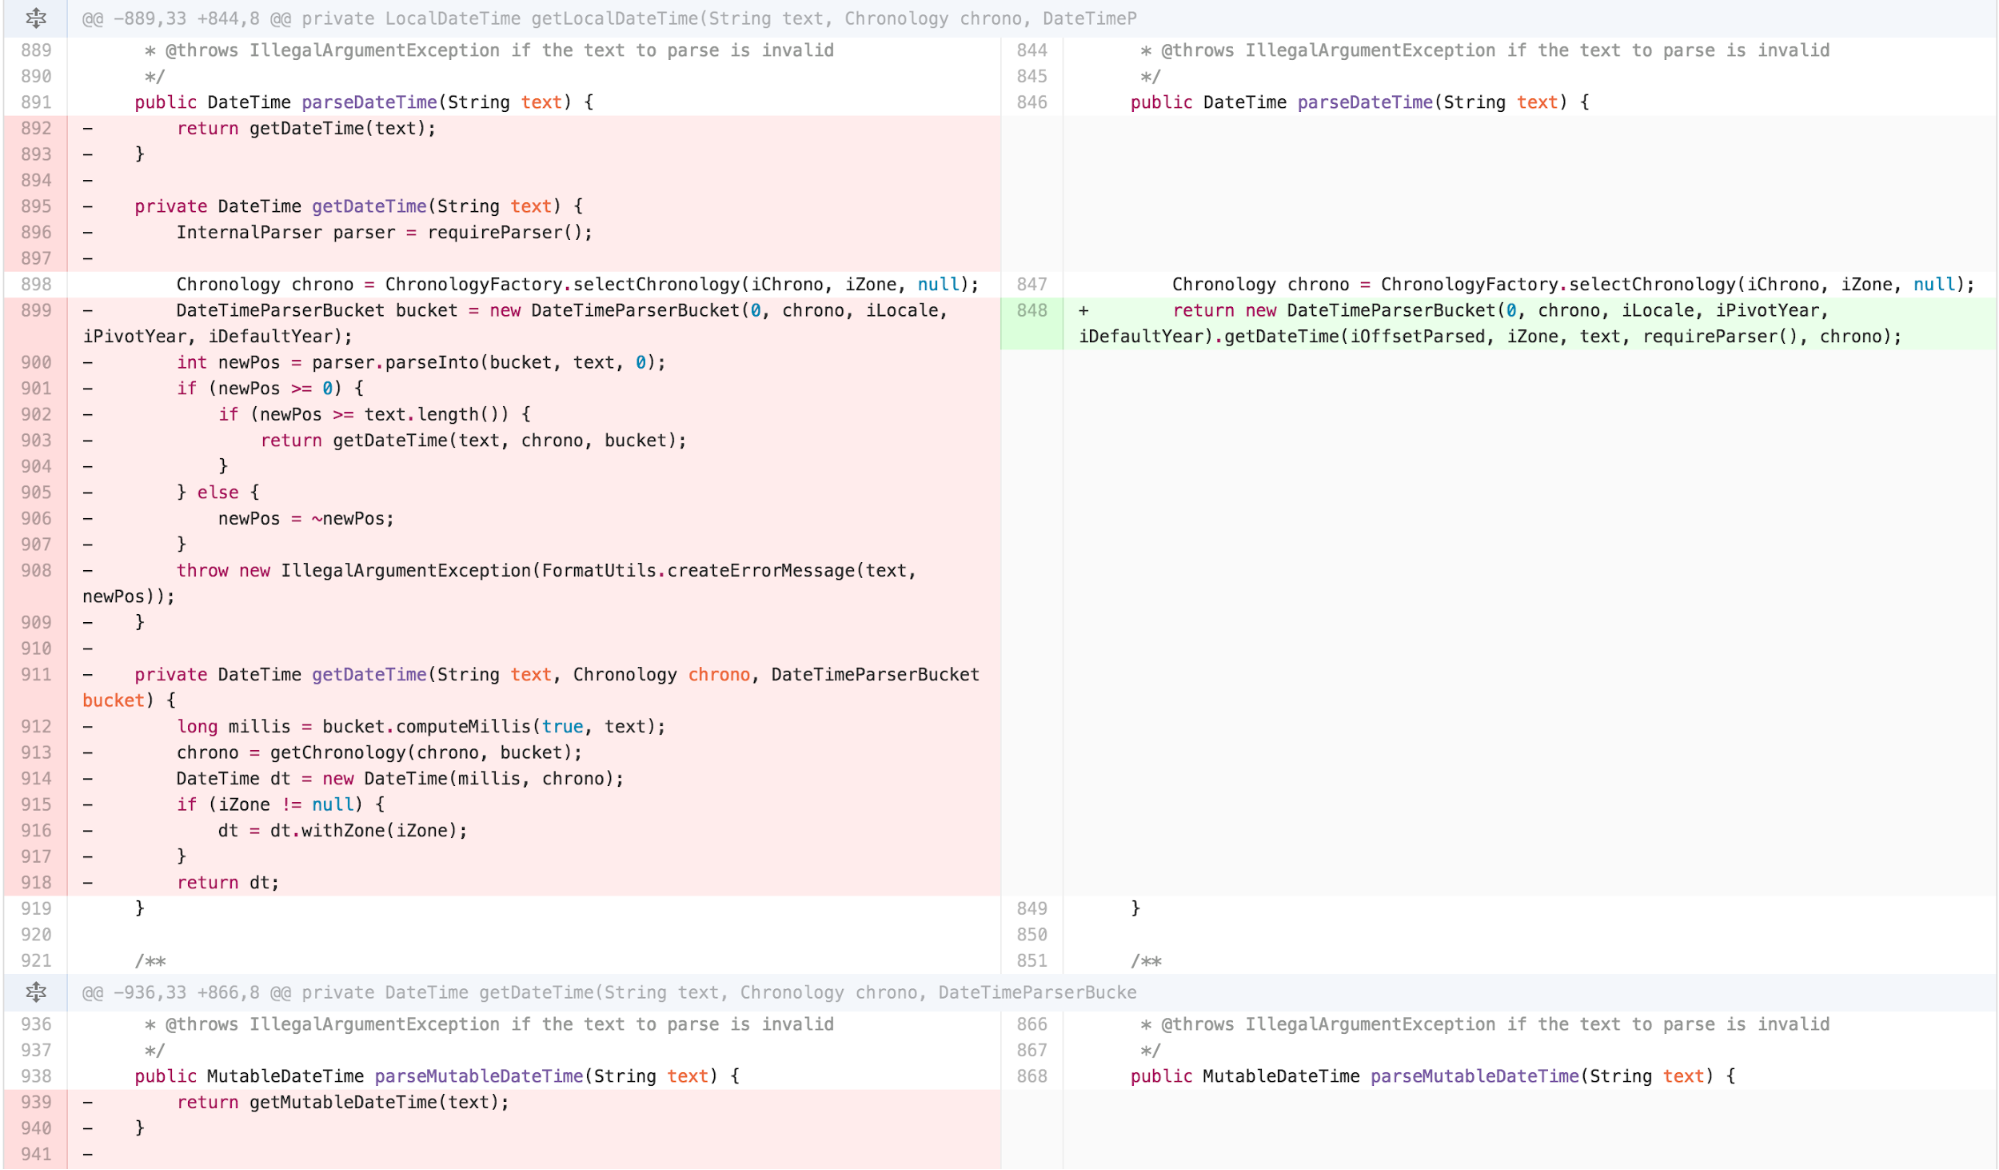
\includegraphics[width=\linewidth]{code48}
	\caption{insert caption}
\end{figure}
\begin{figure}[H]
	\centering
	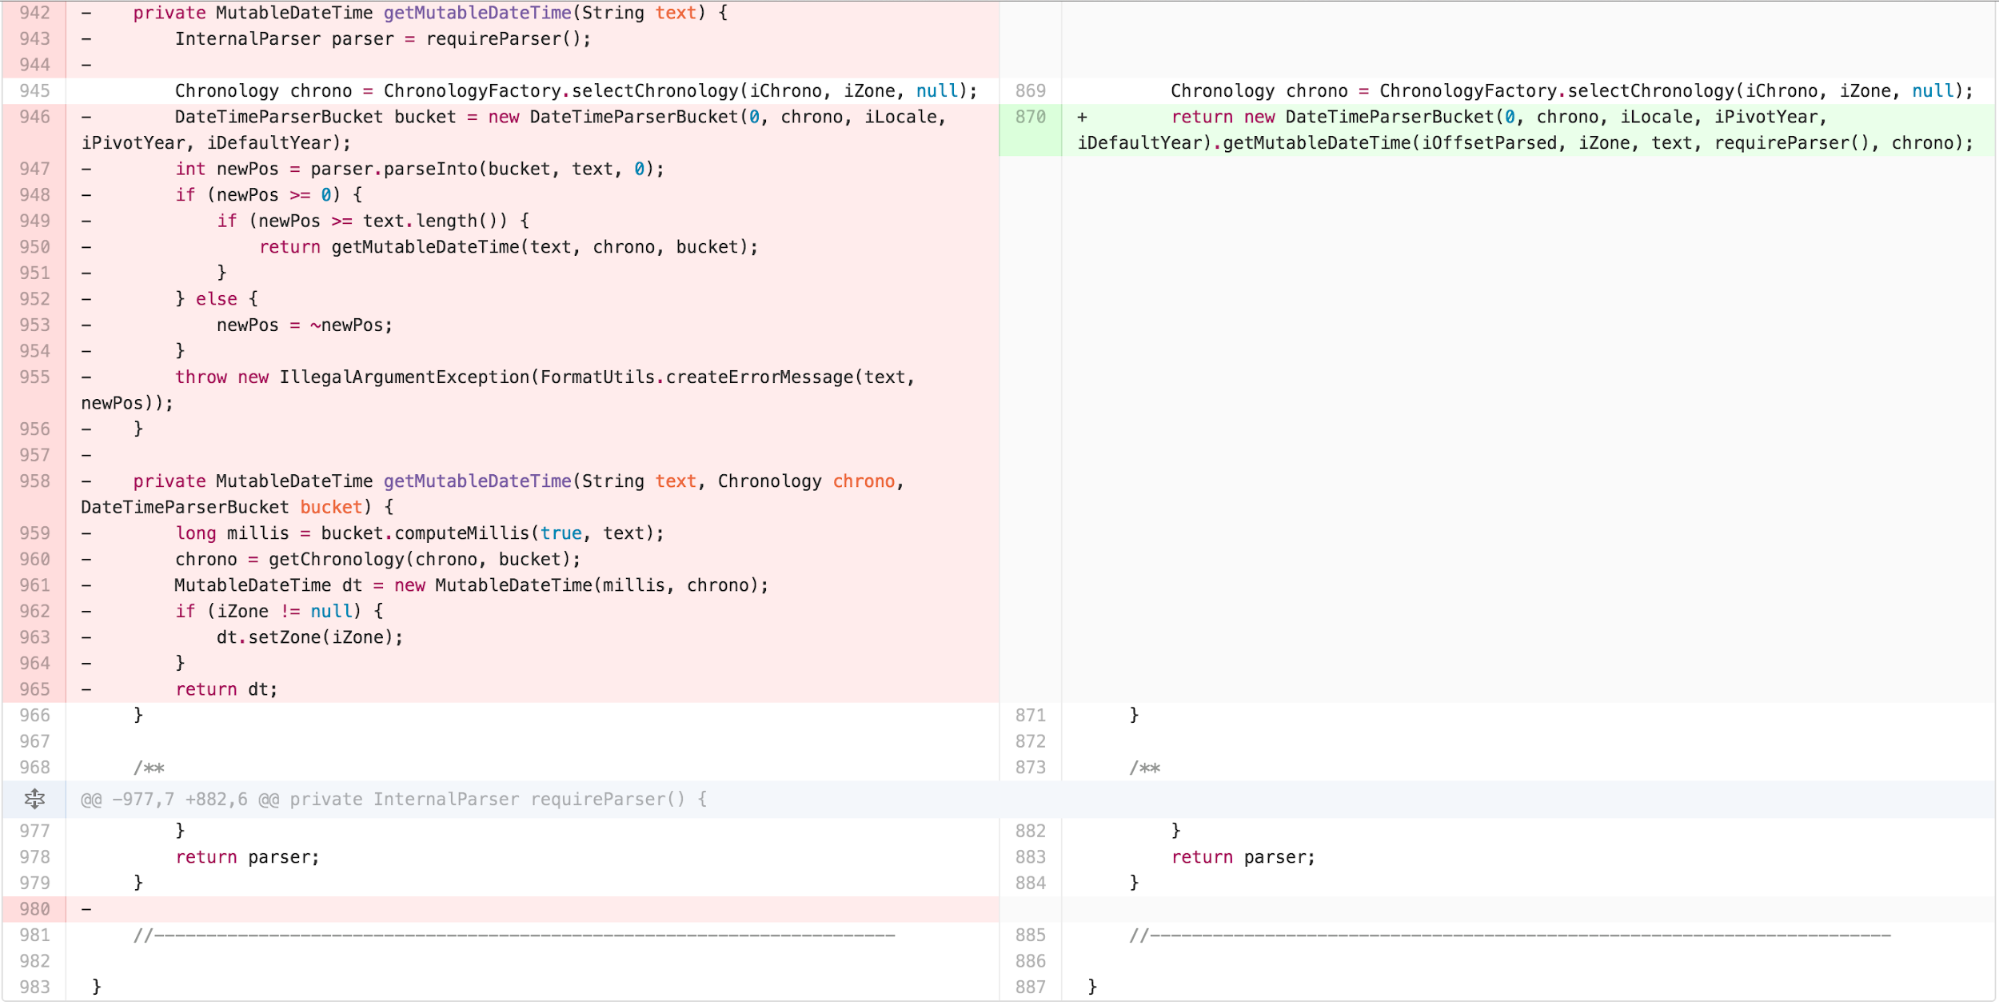
\includegraphics[width=\linewidth]{code49}
	\caption{insert caption}
\end{figure}
\begin{figure}[H]
	\centering
	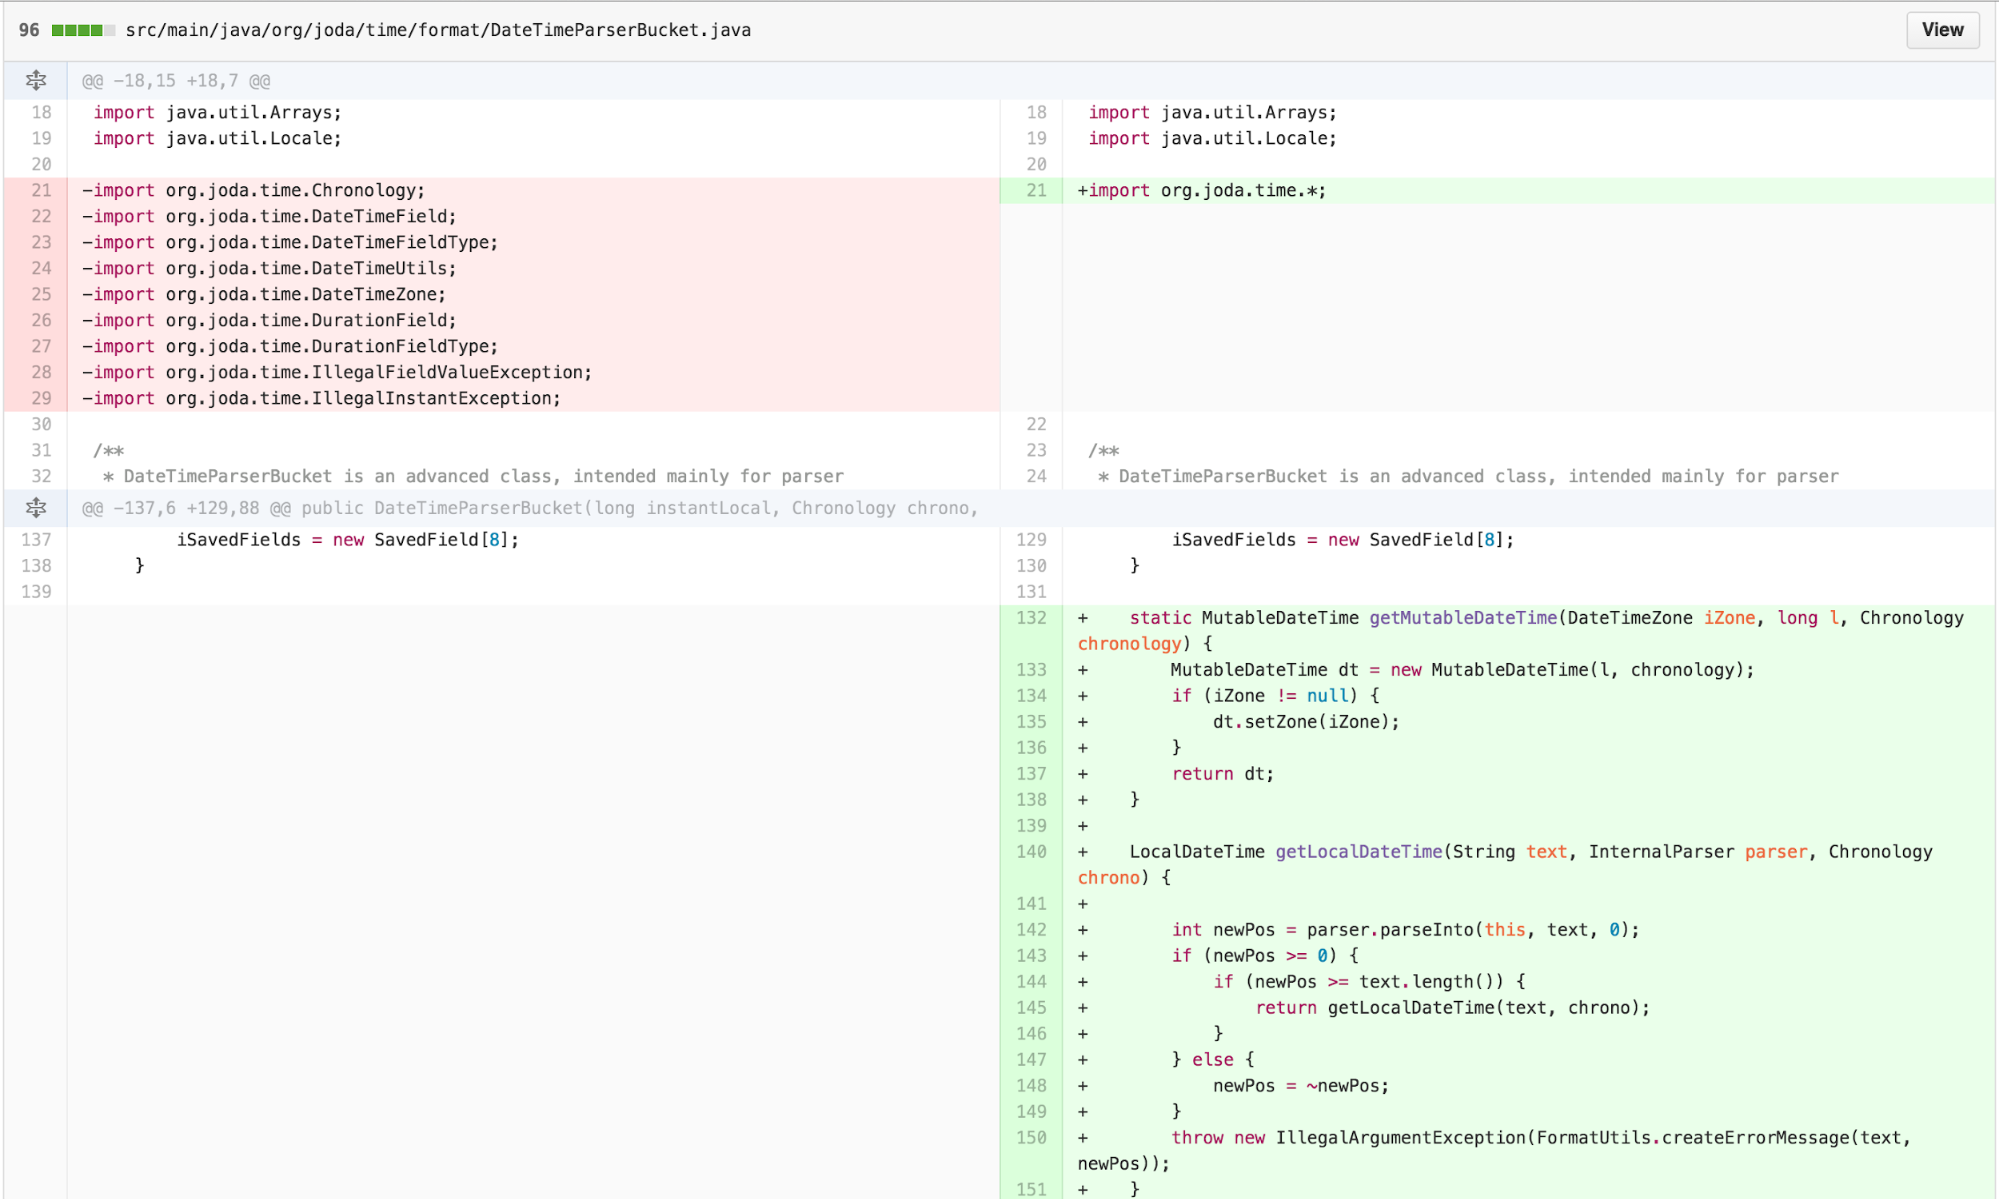
\includegraphics[width=\linewidth]{code50}
	\caption{insert caption}
\end{figure}
\begin{figure}[H]
	\centering
	\includegraphics[width=\linewidth]{code51}
	\caption{insert caption}
\end{figure}
\begin{figure}[H]
	\centering
	\includegraphics[width=\linewidth]{code52}
	\caption{insert caption}
\end{figure}

At this point, I recognized that much of the logic in \texttt{parseIntoInstant} in \texttt{DateTimeFormatter} was similar to the other parsing methods. \texttt{DateTimeFormatter} also found itself doing more work in its internals than necessary because the \texttt{ReadWriteableInstant} interface was missing an update feature. As that functionality seems implied by the name, I added it to the interface and pushed some responsibility onto \texttt{MutableDateTime}.

\begin{figure}[H]
	\centering
	\includegraphics[width=\linewidth]{code53}
	\caption{insert caption}
\end{figure}
\begin{figure}[H]
	\centering
	\includegraphics[width=\linewidth]{code54}
	\caption{insert caption}
\end{figure}
\begin{figure}[H]
	\centering
	\includegraphics[width=\linewidth]{code55}
	\caption{insert caption}
\end{figure}

At this point, I was able to push the entire responsibility of parsing into the \texttt{Instant} into \texttt{DateTimeParserBucket}.

\begin{figure}[H]
	\centering
	\includegraphics[width=\linewidth]{code56}
	\caption{insert caption}
\end{figure}
\begin{figure}[H]
	\centering
	\includegraphics[width=\linewidth]{code57}
	\caption{insert caption}
\end{figure}

\texttt{DateTimeFormatter}’s parse methods were now doing very little besides using its state to set up a \texttt{DateTimeParserBucket}. It seemed like \texttt{DateTimeParserBucket} could be the permanent home of much of this functionality. I could move the functionality over. Along the way, I could start by removing some of the cognitive complexity of \texttt{ChronologyFactory}’s reassignment to input parameters simultaneously.

\begin{figure}[H]
	\centering
	\includegraphics[width=\linewidth]{code58}
	\caption{insert caption}
\end{figure}
\begin{figure}[H]
	\centering
	\includegraphics[width=\linewidth]{code59}
	\caption{insert caption}
\end{figure}
\begin{figure}[H]
	\centering
	\includegraphics[width=\linewidth]{code60}
	\caption{insert caption}
\end{figure}
\begin{figure}[H]
	\centering
	\includegraphics[width=\linewidth]{code61}
	\caption{insert caption}
\end{figure}
\begin{figure}[H]
	\centering
	\includegraphics[width=\linewidth]{code62}
	\caption{insert caption}
\end{figure}

At this point, it felt like I was succeeding more in moving complexity around than removing it. \texttt{DateTimeParserBucket} had most of the functionality related to parsing moved to it, as its internal state was a big part of most of the calculations. But I was no closer to my originally envisioned TEMPLATE METHOD. I also worried that more responsibility on an originally used intermediate calculation scratchpad object may belie its importance in the process. I sought further simplification. I started by reducing the scope of some methods of \texttt{DateTimeParserBucket} and re-arranging them according to the Newspaper Metaphor.

\begin{figure}[H]
	\centering
	\includegraphics[width=\linewidth]{code63}
	\caption{insert caption}
\end{figure}
\begin{figure}[H]
	\centering
	\includegraphics[width=\linewidth]{code64}
	\caption{insert caption}
\end{figure}
\begin{figure}[H]
	\centering
	\includegraphics[width=\linewidth]{code65}
	\caption{insert caption}
\end{figure}
\begin{figure}[H]
	\centering
	\includegraphics[width=\linewidth]{code66}
	\caption{insert caption}
\end{figure}

This helped me identify that the best approach for getting to the desired architecture was to split apart the functionality that had migrated into \texttt{DateTimeParserBucket} into another collaborating object.

\begin{figure}[H]
	\centering
	\includegraphics[width=\linewidth]{code67}
	\caption{insert caption}
\end{figure}
\begin{figure}[H]
	\centering
	\includegraphics[width=\linewidth]{code68}
	\caption{insert caption}
\end{figure}
\begin{figure}[H]
	\centering
	\includegraphics[width=\linewidth]{code69}
	\caption{insert caption}
\end{figure}
\begin{figure}[H]
	\centering
	\includegraphics[width=\linewidth]{code70}
	\caption{insert caption}
\end{figure}
\begin{figure}[H]
	\centering
	\includegraphics[width=\linewidth]{code71}
	\caption{insert caption}
\end{figure}
\begin{figure}[H]
	\centering
	\includegraphics[width=\linewidth]{code72}
	\caption{insert caption}
\end{figure}
\begin{figure}[H]
	\centering
	\includegraphics[width=\linewidth]{code73}
	\caption{insert caption}
\end{figure}
\begin{figure}[H]
	\centering
	\includegraphics[width=\linewidth]{code74}
	\caption{insert caption}
\end{figure}
\begin{figure}[H]
	\centering
	\includegraphics[width=\linewidth]{code75}
	\caption{insert caption}
\end{figure}

With the new delegate \texttt{SimpleParser} in place, I had a target to move towards the desired TEMPLATE METHOD hierarchy. First, I started by inlining some methods I’d previously broken out. Refactoring operations are often well-known to be reversible, as exploring in one direction can lead to realization that the best path was another. I also applying some EXTRACT PARAMETER to reduce the length of method signatures, as the cognitive complexity of methods rises with the length its signature.

\begin{figure}[H]
	\centering
	\includegraphics[width=\linewidth]{code76}
	\caption{insert caption}
\end{figure}
\begin{figure}[H]
	\centering
	\includegraphics[width=\linewidth]{code77}
	\caption{insert caption}
\end{figure}
\begin{figure}[H]
	\centering
	\includegraphics[width=\linewidth]{code78}
	\caption{insert caption}
\end{figure}
\begin{figure}[H]
	\centering
	\includegraphics[width=\linewidth]{code79}
	\caption{insert caption}
\end{figure}
\begin{figure}[H]
	\centering
	\includegraphics[width=\linewidth]{code80}
	\caption{insert caption}
\end{figure}
\begin{figure}[H]
	\centering
	\includegraphics[width=\linewidth]{code81}
	\caption{insert caption}
\end{figure}
\begin{figure}[H]
	\centering
	\includegraphics[width=\linewidth]{code82}
	\caption{insert caption}
\end{figure}
\begin{figure}[H]
	\centering
	\includegraphics[width=\linewidth]{code83}
	\caption{insert caption}
\end{figure}
\begin{figure}[H]
	\centering
	\includegraphics[width=\linewidth]{code84}
	\caption{insert caption}
\end{figure}

Now there was obvious duplication and an outline structure in the body of the \texttt{parse*} methods. I was now able to apply EXTRACT METHOD to identify the points that varied.

\begin{figure}[H]
	\centering
	\includegraphics[width=\linewidth]{code85}
	\caption{insert caption}
\end{figure}
\begin{figure}[H]
	\centering
	\includegraphics[width=\linewidth]{code86}
	\caption{insert caption}
\end{figure}
\begin{figure}[H]
	\centering
	\includegraphics[width=\linewidth]{code87}
	\caption{insert caption}
\end{figure}
\begin{figure}[H]
	\centering
	\includegraphics[width=\linewidth]{code88}
	\caption{insert caption}
\end{figure}
\begin{figure}[H]
	\centering
	\includegraphics[width=\linewidth]{code89}
	\caption{insert caption}
\end{figure}
\begin{figure}[H]
	\centering
	\includegraphics[width=\linewidth]{code90}
	\caption{insert caption}
\end{figure}
\begin{figure}[H]
	\centering
	\includegraphics[width=\linewidth]{code91}
	\caption{insert caption}
\end{figure}
\begin{figure}[H]
	\centering
	\includegraphics[width=\linewidth]{code92}
	\caption{insert caption}
\end{figure}
\begin{figure}[H]
	\centering
	\includegraphics[width=\linewidth]{code93}
	\caption{insert caption}
\end{figure}
\begin{figure}[H]
	\centering
	\includegraphics[width=\linewidth]{code94}
	\caption{insert caption}
\end{figure}

I then had a couple of options. The traditional TEMPLATE METHOD approach would require refactoring the \texttt{SimpleParser} to be a fully-fledged object instead of a utility class full of static methods. This approach required some intensive structural modifications, though is fairly straightforward. However, it is an approach most optimally suited for a traditional object-oriented programming paradigm. 

Functional Programming is experiencing a revival in the software engineering community. As Moore’s Law runs into physical nanoscale limitations, chip manufacturers have sought to improve speeds by increasing the number of cores on a chip and promoting parallel computing. Pure, stateless functions are easier to parallelize. Hence, languages like Ruby, Python, Javascript, Scala, and Clojure began supporting functional paradigms. Eventually, both Java 8 and C++ 11 added functional support features. Many young programmers learning today may have more experience with functional idioms than in the past.

One common functional idiom is the notion of a callback function. When using callbacks, one passes a function to be invoked to another function. The other function is then able to execute and invoke the passed function at its leisure. I explored this approach with a subsequent set of refactoring.

With some slight caveats to handle the difference in exception handling introduced by Java’s Callable, this approach compiles and executes successfully. The question is, is it simpler?

Callbacks are often argued to make code harder to understand. Some argue that they can be used effectively and comprehensibly if the number is limited. There is no data comparing the cognitive load induced by following such an approach versus traditional OOP. This seems like ground rife for future research.

Returning our attention to simplifying the usage patterns, an obvious opportunity to reduce the Split Attention Effect is to use constructor chaining when the initialization semantics are the same and the only difference is a variable number of arguments. Hence, we can simplify one of the \texttt{DateTimeFormatter} constructors as follows.

\begin{figure}[H]
	\centering
	\includegraphics[width=\linewidth]{code95}
	\caption{insert caption}
\end{figure}

We can also significantly simplify the signatures of \texttt{SimpleParser} when we realize that most of its arguments are pulled from \texttt{DateTimeFormatter}.

\begin{figure}[H]
	\centering
	\includegraphics[width=\linewidth]{code96}
	\caption{insert caption}
\end{figure}

This significantly simplifies \texttt{DateTimeParserBucket}:
 
\begin{figure}[H]
	\centering
	\includegraphics[width=\linewidth]{code97}
	\caption{insert caption}
\end{figure}

\texttt{SimpleParser} then provides a FACADE that wraps its callback generation and generalized \texttt{getResult} method.

\begin{figure}[H]
	\centering
	\includegraphics[width=\linewidth]{code98}
	\caption{insert caption}
\end{figure}
\begin{figure}[H]
	\centering
	\includegraphics[width=\linewidth]{code99}
	\caption{insert caption}
\end{figure}
\begin{figure}[H]
	\centering
	\includegraphics[width=\linewidth]{code100}
	\caption{insert caption}
\end{figure}
\begin{figure}[H]
	\centering
	\includegraphics[width=\linewidth]{code101}
	\caption{insert caption}
\end{figure}

At this point, we are ready to apply our instance transformation to form a TEMPLATE METHOD and have individual STRATEGY implementations for each return type.

\begin{figure}[H]
	\centering
	\includegraphics[width=\linewidth]{code102}
	\caption{insert caption}
\end{figure}
\begin{figure}[H]
	\centering
	\includegraphics[width=\linewidth]{code103}
	\caption{insert caption}
\end{figure}
\begin{figure}[H]
	\centering
	\includegraphics[width=\linewidth]{code104}
	\caption{insert caption}
\end{figure}
\begin{figure}[H]
	\centering
	\includegraphics[width=\linewidth]{code105}
	\caption{insert caption}
\end{figure}
\begin{figure}[H]
	\centering
	\includegraphics[width=\linewidth]{code106}
	\caption{insert caption}
\end{figure}
\begin{figure}[H]
	\centering
	\includegraphics[width=\linewidth]{code107}
	\caption{insert caption}
\end{figure}
\begin{figure}[H]
	\centering
	\includegraphics[width=\linewidth]{code108}
	\caption{insert caption}
\end{figure}
\begin{figure}[H]
	\centering
	\includegraphics[width=\linewidth]{code109}
	\caption{insert caption}
\end{figure}
\begin{figure}[H]
	\centering
	\includegraphics[width=\linewidth]{code110}
	\caption{insert caption}
\end{figure}

At this point, we’ve replaced the \texttt{SimpleParser} with a \texttt{ParsingStrategy} and a \texttt{FormatterParsingStrategy} that holds the guts of the \texttt{getResult} method, with subclass implementations for each return type. 

I now also had a straightforward point to simplify common logic. I also had an interface that I could use to unify the differences between the API design of \texttt{parseInto} which mutates the input parameter and returns the resulting position, and the other \texttt{parse} methods. This reduces the architectural complexity of \texttt{DateTimeFormatter} by making all of the parsing follow a common pattern.

\begin{figure}[H]
	\centering
	\includegraphics[width=\linewidth]{code111}
	\caption{insert caption}
\end{figure}
\begin{figure}[H]
	\centering
	\includegraphics[width=\linewidth]{code112}
	\caption{insert caption}
\end{figure}
\begin{figure}[H]
	\centering
	\includegraphics[width=\linewidth]{code113}
	\caption{insert caption}
\end{figure}

When I first tried to make the \texttt{ReadWritableInstantParsingStrategy}, I tried directly extending \texttt{FormatterParsingStrategy} like the other implementations. When I ran the tests, they failed. Something was different about the way it worked. Luckily, having a separate interface for \texttt{ParsingStrategy} from the abstract class implementation of \texttt{FormatterParsingStrategy} allowed me to move forward to advance architectural similarity without being blocked. I was able to create the implementation with only slight duplication of work done in the \texttt{FormatterParsingStrategy}. When I think about it further, it seems like the primary differences between \texttt{ReadWritableInstantParsingStrategy} and the other implementations is that the starting number of milliseconds for the \texttt{DateTimeParserBucket} is not 0, and neither is the position for the \texttt{DateTimeParser}. I could’ve spent some time refactoring \texttt{FormatterParsingStrategy} to parametrize it such that \texttt{ReadWritableInstantParsingStrategy} could extend it. I decided not to because this code path is unlikely to get explored during the study and the goal of this work was to simplify \texttt{DateTimeFormatter}.

\subsection{Signaling architecture by organization -- using packages as chunks}

I now had a simpler \texttt{DateTimeFormatter} whose parsing methods delegated to implementations of parsing STRATEGY. However, the package org.joda.time.format had grown more imposing by adding all of these new classes. We can use packages to organize classes, again applying the concepts of sequencing and chunking to manage how much context a programmer needs to keep in their head at one time. Hence, we add a new package org.joda.time.format.parsing and move the new classes over.

\begin{figure}[H]
	\centering
	\includegraphics[width=\linewidth]{code114}
	\caption{insert caption}
\end{figure}
\begin{figure}[H]
	\centering
	\includegraphics[width=\linewidth]{code115}
	\caption{insert caption}
\end{figure}
\begin{figure}[H]
	\centering
	\includegraphics[width=\linewidth]{code116}
	\caption{insert caption}
\end{figure}
\begin{figure}[H]
	\centering
	\includegraphics[width=\linewidth]{code117}
	\caption{insert caption}
\end{figure}
\begin{figure}[H]
	\centering
	\includegraphics[width=\linewidth]{code118}
	\caption{insert caption}
\end{figure}
\begin{figure}[H]
	\centering
	\includegraphics[width=\linewidth]{code119}
	\caption{insert caption}
\end{figure}
\begin{figure}[H]
	\centering
	\includegraphics[width=\linewidth]{code120}
	\caption{insert caption}
\end{figure}
\begin{figure}[H]
	\centering
	\includegraphics[width=\linewidth]{code121}
	\caption{insert caption}
\end{figure}

Another heuristic to reduce the number of classes is to find LAZY CLASS and investigate whether we can MOVE METHOD. As \texttt{ChronologyFactory} is merely exposing a method that could be a STATIC FACTORY METHOD on \texttt{Chronology}, we move the functionality over.

\begin{figure}[H]
	\centering
	\includegraphics[width=\linewidth]{code122}
	\caption{insert caption}
\end{figure}
\begin{figure}[H]
	\centering
	\includegraphics[width=\linewidth]{code123}
	\caption{insert caption}
\end{figure}
\begin{figure}[H]
	\centering
	\includegraphics[width=\linewidth]{code124}
	\caption{insert caption}
\end{figure}

\subsection{Making Derived Components Expressive, the value of names}
Are we done? The resultant code is structurally simpler than before. The outstanding question is, does it communicate the design intent of the original algorithm in a concise and clear way? Without access to the direct authors of the code and given the complexity of the original, it’s difficult to say. Debugging through the code flow into the area of the bug, we see much of the code is now delegation: \texttt{DateTimeFormatter} -\textgreater DateTimeParsingStrategy -\textgreater FormatterParsingStrategy -\textgreater NumberFormatter -\textgreater OffsetCalculator. Most of the work involved in this bug is in the OffsetCalculator...could the code be clearer?

Consultation with other engineers suggested that the OffsetCalculator has variable names that were mostly consequential to its original sources. Revisiting those names may enhance clarity. Additionally, much of the work of calculateLength is done once, ultimately to be used by calcluateValue. This work can be moved to the constructor, with expressive variables assigned. I can clean this up further.

\begin{figure}[H]
	\centering
	\includegraphics[width=\linewidth]{code125}
	\caption{insert caption}
\end{figure}
\begin{figure}[H]
	\centering
	\includegraphics[width=\linewidth]{code126}
	\caption{insert caption}
\end{figure}
\begin{figure}[H]
	\centering
	\includegraphics[width=\linewidth]{code127}
	\caption{insert caption}
\end{figure}
\begin{figure}[H]
	\centering
	\includegraphics[width=\linewidth]{code128}
	\caption{insert caption}
\end{figure}
\begin{figure}[H]
	\centering
	\includegraphics[width=\linewidth]{code129}
	\caption{insert caption}
\end{figure}

The clearer variable names and re-arranged methods lead me to realize there is a clean separation between two distinct concepts missing in the OffsetCalculator. Much of the work it does results from FEATURE ENVY of the CharSequence. Procedural style code that asks questions such as “does the text begin with a + or -?” would be better answered independently from the calculation.

\subsection{The Final Form -- calculate in the NumberFormatter, NumericSequence}

I can decompose the OffsetCalculator back into a data type that provides the necessary functionality on top of CharSequence and a calculation that uses that data type to calculate a value in the NumberFormatter implementation of InternalParser. This aligns most well with the Cognitive Load Theory principle of “write high cohesive content for low-knowledge learners.”  

\begin{figure}[H]
	\centering
	\includegraphics[width=\linewidth]{code130}
	\caption{insert caption}
\end{figure}
\begin{figure}[H]
	\centering
	\includegraphics[width=\linewidth]{code131}
	\caption{insert caption}
\end{figure}
\begin{figure}[H]
	\centering
	\includegraphics[width=\linewidth]{code132}
	\caption{insert caption}
\end{figure}
\begin{figure}[H]
	\centering
	\includegraphics[width=\linewidth]{code133}
	\caption{insert caption}
\end{figure}
\begin{figure}[H]
	\centering
	\includegraphics[width=\linewidth]{code134}
	\caption{insert caption}
\end{figure}
\begin{figure}[H]
	\centering
	\includegraphics[width=\linewidth]{code135}
	\caption{insert caption}
\end{figure}
\begin{figure}[H]
	\centering
	\includegraphics[width=\linewidth]{code136}
	\caption{insert caption}
\end{figure}
\begin{figure}[H]
	\centering
	\includegraphics[width=\linewidth]{code137}
	\caption{insert caption}
\end{figure}
 
\section{The Experimental Solution}

This has been a lot of work! But the resulting solution is very satisfying. In fact, it requires adding no additional code. The correct solution to fixing the bug actually involves removing some existing confusing code.

\begin{figure}[H]
	\centering
	\includegraphics[width=\linewidth]{code138}
	\caption{insert caption}
\end{figure}

Just like that, the bug is resolved.
 
\subsection{Side-by-Side comparison}

According to SonarQube 5.4, the metrics for the experimental version are shown below.

\begin{figure}[H]
	\centering
	\includegraphics[width=\linewidth]{metric1}
	\caption{insert caption}
\end{figure}
\begin{figure}[H]
	\centering
	\includegraphics[width=\linewidth]{metric2}
	\caption{insert caption}
\end{figure}
\begin{figure}[H]
	\centering
	\includegraphics[width=\linewidth]{metric3}
	\caption{insert caption}
\end{figure}
\begin{figure}[H]
	\centering
	\includegraphics[width=\linewidth]{metric4}
	\caption{insert caption}
\end{figure}

Comparing these with the original DateTimeFormatter and DateTimeFormatterBuilder;  

\begin{figure}[H]
	\centering
	\includegraphics[width=\linewidth]{metric5}
	\caption{insert caption}
\end{figure}
\begin{figure}[H]
	\centering
	\includegraphics[width=\linewidth]{metric6}
	\caption{insert caption}
\end{figure}

From a pure complexity metrics perspective, it doesn’t look like much has changed. DateTimeFormatterBuilder went from a control complexity score of 550 to 543 in the experimental. The complexity per function dropped from 3.5 from to 3.4. The number of lines of code dropped by 21. The number of duplications dropped from 2.3\% to 0.7\%.
 
DateTimeFormatter shows a slightly more pronounced effect. The complexity score dropped from 98 to 64. The complexity per function went from 2.5 to 1.7. The number of lines of code dropped by 110. The 2.9\% duplications dropped to 0.

Are these changes enough to show a measurable difference in comprehensibility and debugging time? If current best practice software engineering complexity metrics are sufficient, I do not expect to find a statistically significant difference. Thus, I am ready to conduct a study. 
